\documentclass[12pt]{article}
\usepackage{tocloft}% to configure the ToC <<<<<
\setlength{\cftsecnumwidth}{4.5ex}% set the width to the section number in the ToC <<<<<
\renewcommand{\thesection}{\Roman{section}.} 
\renewcommand{\thesubsection}{\quad \Alph{subsection}.}
\renewcommand{\thesubsubsection}{\qquad \roman{subsubsection}.}

\usepackage[style=authoryear,bibencoding=auto,strict,backend=biber,natbib,maxcitenames=2]{biblatex}

\usepackage{amssymb,amsmath,amsfonts,bbm,bm,eurosym,geometry,ulem,graphicx,color,setspace,sectsty,comment,float,caption,pdflscape,setspace,subfigure,array,hyperref}
\usepackage{xurl}
\usepackage[font=bf]{caption}
\usepackage{xcolor}
\usepackage[bottom]{footmisc}
\hypersetup{
    colorlinks,
    linkcolor={black},
    citecolor={blue!50!black},
    urlcolor={blue!80!black}
}
\addbibresource{bibliography.bib}

\normalem

\onehalfspacing

\geometry{left=1.0in,right=1.0in,top=1.0in,bottom=1.0in}

\begin{document}

\begin{titlepage}
\title{Staggered Difference-in-Differences Estimation for Antitrust Analysis: A Review of New Literature and Recommendations for Practitioners}
\author{Hassan Faghani\thanks{Berkeley Research Group} \and Steven VanOmmeren\thanks{Berkeley Research Group. \\\\ We thank several colleagues at Berkeley Research Group for providing helpful comments in forming this paper, including [[...]].}}
\date{\today}
\maketitle
\begin{abstract}
\noindent \\
The aim of this paper is twofold: First, we bring antitrust practitioners and applied econometricians up to speed on the new literature surrounding difference-in-differences (DiD) methods. Second, we aim to provide a resource for sound DiD analysis in expert testimony in light of these developments. We review relevant new papers and their most important conclusions. We then discuss the antitrust implications of three important topics: parallel trends, the not-yet-treated group, and data with customer entry and exit. We supplement this discussion with Monte Carlo analysis, in which we compare the performance of DiD estimators and quantify certain types of bias. We discuss the many sensitivities and robustness checks that should underly expert testimony going forward. Along the way, we aim to assist future expert analysis by centralizing the new work and interpreting its results. DiD theory has come a long way in the academic literature since the 2010s, and we distill that knowledge into what we consider to be the new standard for robust DiD results in 2024.\\
\vspace{0in}\\
\noindent\textbf{Keywords:} difference-in-differences, staggered treatment, heterogeneity, antitrust
\vspace{0in}\\
\noindent\textbf{JEL Codes:} C18, C52, L40\\

\bigskip
\end{abstract}
\setcounter{page}{0}
\thispagestyle{empty}
\end{titlepage}
\pagebreak \newpage


\tableofcontents

\doublespacing

\newpage
\section{Introduction} \label{sec:introduction}
Understanding the effects of policy changes is among the fundamental problems of applied social sciences. In economic and legal studies, one of the most popular techniques to measure policy changes is Difference-in-Differences (“DiD”) analysis.\footnote{We wrote a high-level summary of DiD and the new literature developments in early 2023. This paper goes into much more econometric detail and builds intuition for the various new tests and estimators. We also cite several papers that have come out since then. \url{https://www.law360.com/articles/1568455/the-difference-in-differences-antitrust-analysis-is-evolving}.}  At its core, DiD is relatively simple to understand, contributing to its popularity. In DiD, a group of entities, such as firms, stores, or customers, that have been affected by an event of interest are compared against another group of entities that were not affected. We then analyze the trend over time of this difference; a difference (over time) in differences (between the affected and unaffected). DiD essentially combines two common impact methods (yardstick and before-after analysis) to yield a more robust estimate. The underlying assumption is that the studied policy is the only meaningful change between the two groups once the treatment starts. The affected group is referred to as the “treatment group” and the unaffected is the “control group.” A simple DiD visualization is shown below in Figure \ref{fig:did-diagram}.
\begin{figure}[H]
    \centering
    \caption{Example of Simple DiD Analysis}
    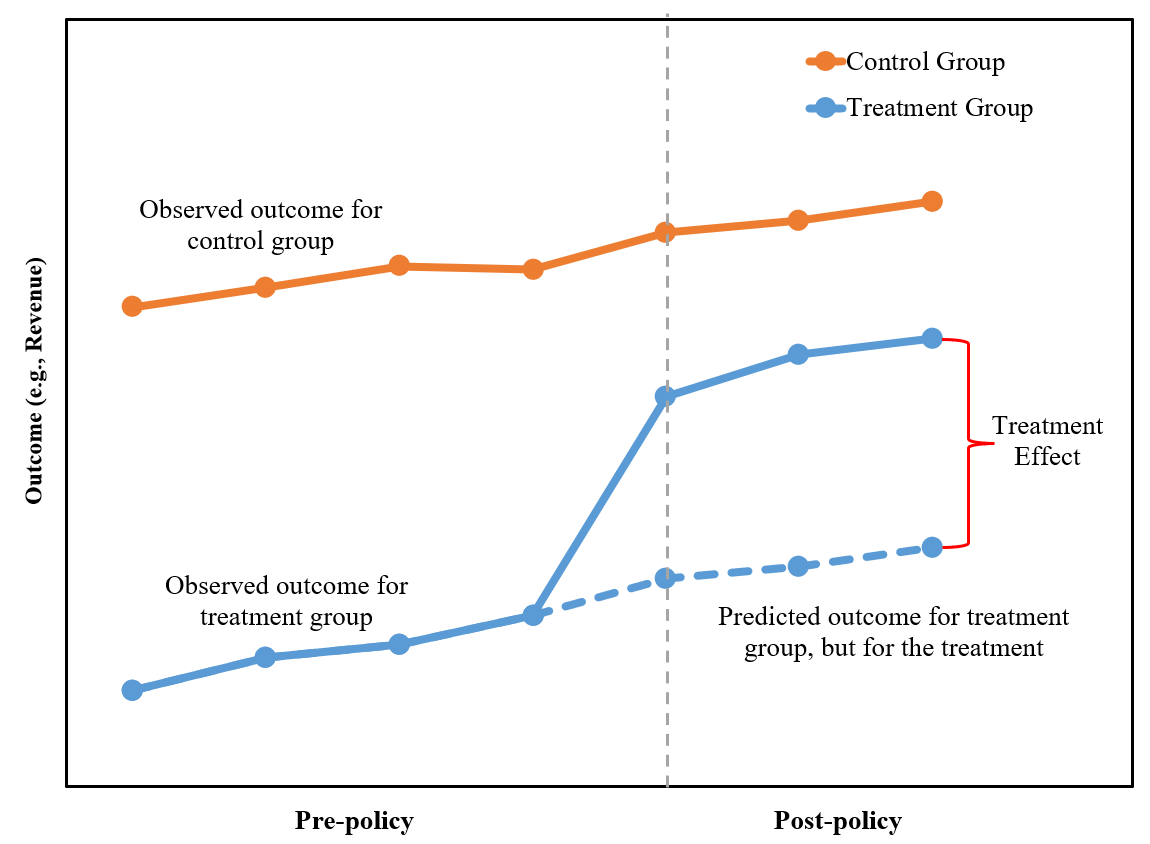
\includegraphics[width=6in]{Figures/Diff in Diff Diagram.PNG}
    \label{fig:did-diagram}
    \vspace{5mm}
    \footnotesize \begin{singlespace*}
        \parbox{5.5in}{A hypothetical DiD example. Here, the treatment group experiences a policy change starting at the dashed vertical line. To calculate the average treatment effect, we compare the difference pre/post for the control group with that of the treatment group. The dashed blue line represents how the treatment group would have moved if it followed the control group’s behavior in the post-treatment period.}
    \end{singlespace*}
\end{figure}
\noindent
DiD is commonly used in a variety of antitrust analyses. For example, it can measure the harm from illegal conduct by modelling changes in revenue; this framework was used to estimate overcharges and damages from alleged anticompetitive behavior in the market for data management systems.\footnote{\textit{In re Dealer Management Systems Antitrust Litigation}, 581 F.Supp.3d 1029 (N.D.Ill., 2022). Part of the \textit{Daubert} challenge against Plaintiffs’ experts involved assessing a violation of the parallel trends assumption. \textit{Id} at 69.}  DiD was used to estimate overcharges to manufacturers from an alleged conspiracy to raise prices of coupon-processing fees.\footnote{\textit{Mr. Dee's Inc. v. Inmar, Inc.}, 2021 WL 4224720 (M.D.N.C., 2021), at *5. Plaintiff’s expert supplemented the DiD analysis with both a before-after (difference over time) and yardstick approach (contemporaneous difference between treatment and control). }  DiD measured whether Staples stores’ prices were lower when they faced local competition from Office Depot.\footnote{\citet{ashenfelter2004} Equations 2 through 5 (Discussing  \textit{Federal Trade Commission v. Staples, Inc.}, 970 F. Supp. 1066 (D.D.C. 1997)). While not described as such, these regressions are forms of two-way fixed effects (“TWFE”) models, which is a type of DiD analysis.}  And it was used to assess “whether and to what extent NorthShore's post-merger price increases were the result of increased market power resulting from the merger [with Highland Park Hospital].”\footnote{\textit{In re NorthShore Univ. HealthSystem Antitrust Litig.}, No. 07-cv-4446, 2018 WL 2383098, at *2, citing \textit{Messner}, 669 F.3d at 818. Interestingly, there was much debate over whether Plaintiff’s DiD analysis would be valid in the presence of non-uniform (i.e. heterogeneous) price increases, a subject of interest in the new literature.} 

DiD isolates the average effect of a policy change only under certain assumptions. The most prominent assumption is that the treatment group would have followed the same relative path as the control group absent the policy change. This assumption is called the \textbf{parallel} or \textbf{common trends assumption}. Equivalently, DiD attributes any change in the treatment group as being due to the policy change; it assumes that all other meaningful events are controlled for. Failing the parallel trends assumption can call into question the validity of DiD results and makes causal interpretation more difficult. This assumption is often a central topic of critique when DiD is used in antitrust analysis, and it can make or break a model. In practice, it is near impossible to find a control group that moves identically to the treatment group, as there will always be some observable differences between the two. However, econometricians have still extracted useful information from DiD models, adding caveats about uncertainty to their results rather than rejecting them entirely. We discuss how parallel trends tests and assumptions are affected by the new literature in more detail in \hyperref[sec:parallel-trends]{Section IV.A below}.

Research questions are often more complicated than just measuring one average effect, and the nature of the data and policy of interest may further complicate things. To account for these complications, DiD analysis in antitrust is typically implemented with a linear regression, which can also control for observable factors and estimate the statistical significance of results. For example, DiD analysis of prices in a conspiracy setting may include additional relevant controls for supply and demand.

One common complication in a DiD framework is differential treatment timing. In this case, different units affected by the policy or conduct start or end their treatment at different times. A special case of differential treatment timing, where the treatment units remain permanently affected after their treatment, is called staggered treatment.\footnote{We examine binary staggered treatment in this paper, which additionally assumes that the treatment effect is immediate and can only be turned on or off. A non-binary treatment example would be drug trials which give different amounts of the drug to different treatment units. Binary treatment is most common in antitrust work, where we usually have no way of knowing or characterizing “how much” of the treatment is happening. However, certain types of non-binary treatment can be effectively estimated by the methods we discuss here. For example, the ramp-up effects of a conspiracy could be captured by measuring treatment effects over time.}  Staggered treatment designs are common in policy evaluation and antitrust analysis. For example, merger analysis may examine price effects surrounding acquisitions in different local markets over time, and price-fixing mechanisms may involve rolling out price increases for certain products over time. A visual timing of a staggered treatment design is shown below in Figure \ref{fig:visual}. Notice how in certain years, there are units that have not yet been affected by the policy change (the “not-yet-treated” group), and others who have. As it turns out, DiD analysis in this setting will use the not-yet-treated group, along with the prototypical control group (called the “never-treated” group), in forming the estimated policy effect. How exactly this works is a focal point of the new literature we discuss below.
\begin{figure}[H]
    \centering
    \caption{Example of Staggered Treatment Mechanism}
    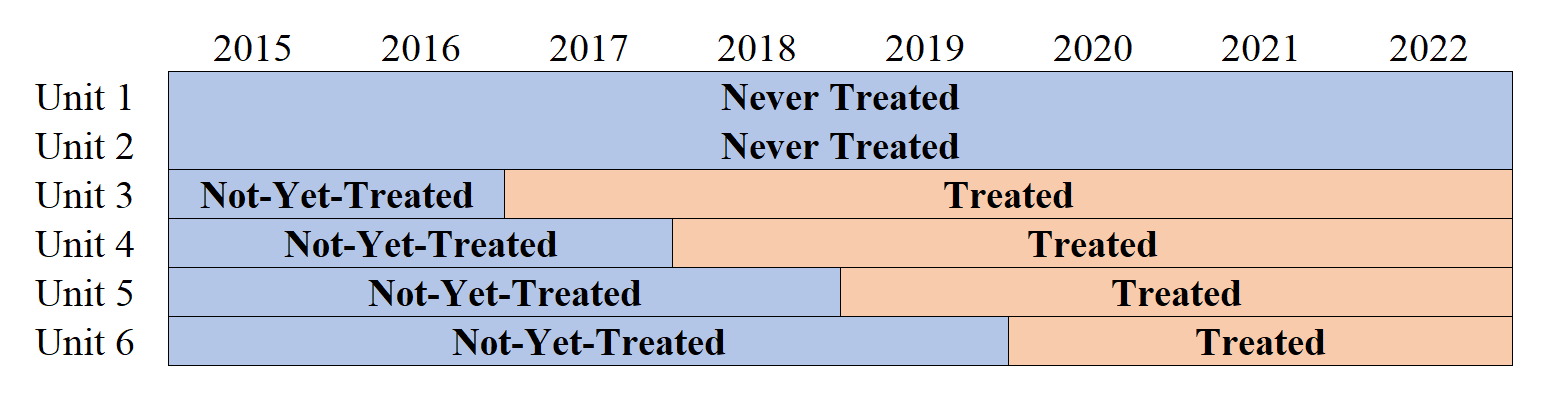
\includegraphics[width=6in]{Figures/Visual Staggered Treatment.PNG}
    \label{fig:visual}
    \vspace{2mm}
    \footnotesize \begin{singlespace*}
        \parbox{5.5in}{In this diagram, each row represents an individual in the data. The first two rows never experience the policy change. The remaining four rows each experience the effects of the policy starting at different times, from 2017 to 2020. In this case, the policy and its treatment effect are staggered across the units.}
    \end{singlespace*}
\end{figure}
\noindent There are also cases where entities in the treatment and the control group can “enter” or “exit” the data for some part of the analysis. In transaction data, it is likely to observe some customers for part of the timeframe of the data; new customers come in and others leave. This can complicate the analysis: are customers leaving the data randomly, or is it because a conspiracy raised the price of their favorite products too much?
One can imagine several other complications of applied DiD analysis. An important question is: how do these complications interact with the policy effect we’re trying to measure? It’s very likely (and sometimes expected by economic theory) that overcharges change over time as the market responds to supracompetitive prices or cartel members attempt to cheat the conspiracy. Certain groups of customers may be easier to overcharge than others, depending on buyer power, asymmetric information, or competitive conditions. It’s also possible that when customers renew long-term contracts well into a conspiracy, their overcharges could differ from customers who renewed during the beginning stages of the conspiracy. All of these examples require special consideration when performing DiD analysis.

A large body of literature on DiD analysis has appeared in recent years which aims to better understand how such complications affect our regression results. Academics have largely confirmed the suspicions of careful applied econometricians by proving that results are biased if we don’t appropriately account for the studied policy and its effects. But of particular interest, the new research has revealed a bias in DiD estimates inherent to the staggered nature of the treatment mechanism, along with other such inherent biases. In the years since, the literature has provided several new estimators that are robust to certain types of misspecifications, detailed sets of assumptions that underly their results, and many other sensitivities and checks to diagnose issues common to DiD analysis.

We review the developments in DiD literature in \hyperref[sec:literature]{Section II}. \hyperref[sec:analysis]{Section III} summarizes the new estimators and tests we think are best suited for antitrust econometric work. Section \hyperref[sec:antitrust]{Section IV} further discusses three topics of particular interest for antitrust practitioners. Results using a Monte Carlo analysis are reported in \hyperref[sec:analysis]{Section V}. In \hyperref[sec:conclusion]{Section VI} we conclude.

\section{Review Of Recent Developments In Staggered DiD} \label{sec:literature}
\begin{singlespace*}
\quote{
    \textit{``The realization that one of the most commonly used empirical methods in social science relies on an often-implausible assumption has spurred a flurry of methodological papers diagnosing the seriousness of the issue, and proposing alternative estimators.''}\footnote{\citet{de2023two}, C2.}
}
\end{singlespace*}
\noindent Our summary of new literature developments comes from the following sources: \citet{baker2022much}, \citet{de2023two}, \citet{roth2023s}, and the authors’ personal research. New papers become available online every week, so more survey work will be needed going forward. Note that the dates associated with these papers can be misleading. For instance, the seminal Goodman-Bacon work was an NBER working paper in 2018,  but it wasn’t published in a peer-reviewed journal until 2021. Many other papers are available online well before they are reviewed and published. As a result, new articles often cite unpublished/preprint work, and many authors are bouncing ideas off each other. We caution that some of the work we discuss is not peer-reviewed, yet it has become so popular that the methods should be known anyways.

However, we think that much of the dust has settled in the staggered, binary treatment DiD space, at least with respect to eliminating the bias associated with “forbidden comparisons” from the staggered assignment. Any future work in this space will likely be improving the new estimators in terms of computational efficiency and robustness to misspecification. But other areas of DiD analysis are wide open and in active development, including continuous treatments, spillover effects, nonlinear treatment effects, and a large interest in the application of machine learning methods to DiD. We leave a discussion and recommendations for these fields to future work.\footnote{For further reading, see \citet{roth2023s}, \citet{de2023two} and references therein.}

A series of econometric papers starting around 2018 closely examined the composition of the DiD coefficient when there are multiple time periods, treatment units, and especially under staggered treatment, i.e. under more realistic scenarios where researchers commonly use DiD. The authors aimed to better understand what the single DiD coefficient identifies for linear models like this (called two-way fixed effects or TWFE models):\footnote{The models are called two-way fixed effects because they have fixed effects (indicator variables for all levels of a categorical variable) for both the time and unit dimensions in the panel.}
\begin{equation}
    y_{it} = \alpha_i + \lambda_t + \boldsymbol{\gamma}  D_{it} + \beta X_{it} + \epsilon_{it},
\end{equation}
Where $y_{it}$ is the outcome of interest, such as price, $\alpha_i$ are unit fixed effects, $\lambda_t$ are time period fixed effects, $D_{it}$ is an indicator variable which is 1 for being actively affected by the policy and 0 otherwise, $X_{it}$ represents other observable variables, and finally $\epsilon_{it}$ captures variations in the data that cannot be explained by the model.\footnote{This model specification is referenced in many popular econometric textbooks, including  \citet{angrist2009mostly}, Section 5.2.1; \citet{hansen2022econometrics}, p. 671; and \citet{cameron2020}, pp. 768-770. \\\\ TWFE is considered a “default” DiD specification when there are multiple groups and time periods. This is often a matter of convenience. Rather than identifying which confounding events or characteristics need to be controlled for in the model, TWFE controls for all time-invariant and unit-invariant heterogeneity. But these fixed effects do not control for time-varying events that affect a subset of the units.}  We note that, unlike the classical DiD (which would include indicators for treatment group, post-policy, and their interaction), TWFE models only include the interaction variable. This is because the unit fixed effects inherently identify the treatment group, and the time fixed effects identify the post-policy period. TWFE automatically “works” even when the treatment is staggered (in that the regression runs), but it’s not obvious what is happening under the hood.

A major breakthrough in understanding the TWFE DiD coefficient is \citet{goodman-bacon2021a}, which proves that the DiD coefficient in a staggered setting is actually a weighted average of many smaller, component DiD coefficients within the data. In fact, it is equal to a weighted average of all possible 2 unit, 2 period (i.e. classical) DiD designs in the data.\footnote{\citet{goodman-bacon2021a}, pp. 257-260 (Theorem 1).}  There are two related results from this knowledge: 1) included in the average are DiD coefficients where a unit that becomes treated at a given time is compared to a “control” unit that is actually already-treated by that point, and 2) some of the weights in the average are unexpectedly negative, and the weights themselves are unintuitive.\footnote{Tests from the literature can recover estimates of these weights, which we describe below.} These types of unexpected DiD coefficients underlying the TWFE coefficient are called “\textbf{forbidden comparisons}.”\footnote{\citet{de2023two}, Section 2.2 (The origin of the problem: ‘forbidden comparisons’).}  An illustration of component DiDs that then form a weighted average in the TWFE regression is shown below. The example has two subjects that are affected by the treatment at different times, and one which is never affected. This implies four component DiD coefficients making up the average.
\begin{figure}[H]
    \centering
    \caption{Illustration of Staggered TWFE Coefficient Comparisons (\citet{goodman-bacon2021a} Figure 2)}
    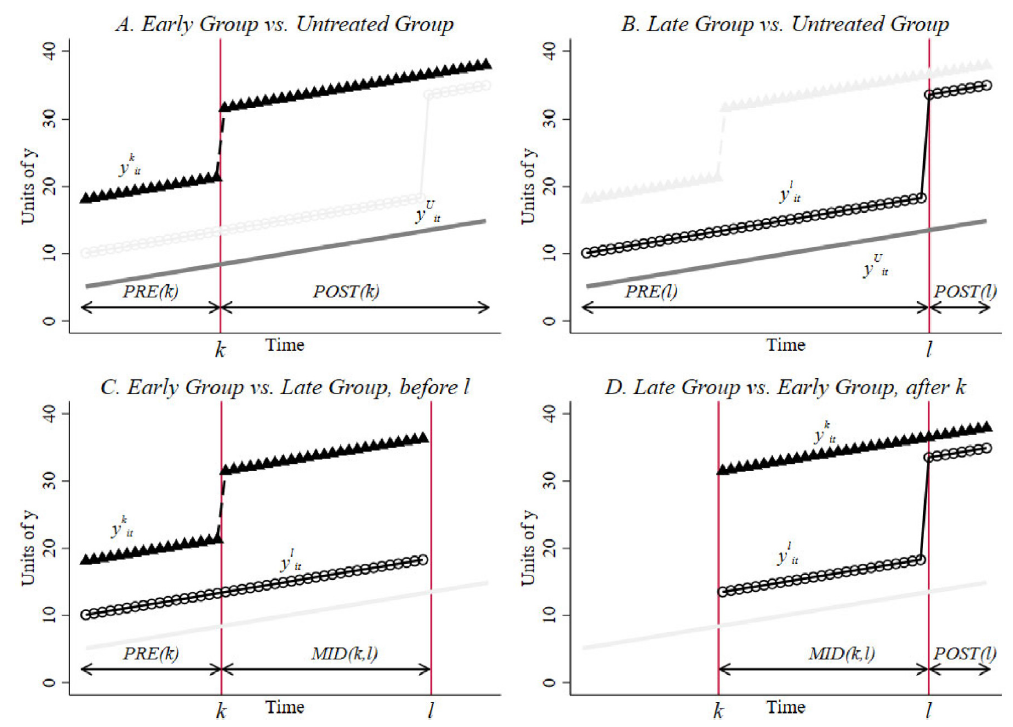
\includegraphics[width=6in]{Figures/Goodman-Bacon (2021) Figure 2.PNG}
    \label{fig:AGB-fig2}
\end{figure}
The four panels form into a single weighted average when running a TWFE model on this data.\footnote{Because the basic 2x2 DiD is (change in treatment group) – (change in control group), we can turn this into an equation (following Prof. Goodman-Bacon’s notation):
\begin{equation*}
    DiD^{TWFE} = w_A\cdot\left(\Delta_k^{y^k} - \Delta_k^{y^U}\right) + w_B\cdot\left(\Delta_l^{y^l} - \Delta_l^{y^U}\right) + w_C\cdot\left(\Delta_k^{y^k} - \Delta_k^{y^l}\right) + w_D\cdot\left(\Delta_l^{y^l} \textcolor{red}{- \Delta_l^{y^k}}\right).
\end{equation*}
Highlighted in red is the negative weight.}  The “control group” used in Panel D is actually the already-treated unit $k$. As a result, part of the post-period effect for treatment unit $k$ is subtracted from the combined DiD estimate, potentially biasing the result.\footnote{\citet{goodman-bacon2021a}, p. 255 (“when already-treated units act as controls, changes in their treatment effects over time get subtracted from the DD estimate.”). In Panel D, $k$ is the already treated unit, and its change in treatment effect over time ($\Delta_l^{y^k}$) is subtracted from $DiD^{TWFE}$. See also, \url{https://friosavila.github.io/playingwithstata/main_csdid.html} (last accessed March 12, 2024).}  This subtraction of treatment effects is a negative weight that stems from a forbidden comparison.

The standard TWFE DiD coefficient is thus susceptible to bias from staggered treatments, and the negative weights can even misrepresent the sign of the true average treatment effect in certain extreme cases, as we discuss next.\footnote{See \citet{de2023two}, pp. 4-6 for a more detailed discussion. They recognize that “no-sign-reversal” (i.e. being robust to this phenomenon) is a desirable property, and this is particularly true for impact evaluation in expert work. We discuss some of the many new techniques to address this issue below. \\\\
Sign reversal is unlikely to occur in practice, but bias associated from negative weights can still substantially alter overcharges or damage estimates.}  Several papers followed in understanding this effect in greater detail, decomposing it in different ways, and providing diagnostic tests and alternative estimators.

\citet{baker2022much} run simulations to demonstrate how the single DiD coefficient can be misleading under various realistic scenarios. In particular, their Simulation 6 shows how the estimated DiD effect can be \textit{negative} even when all treatment effects are \textit{positive}, because of forbidden comparisons in the model.\footnote{See also, \citet{sunshapiro2022a}, Figure 1.}  For example, when the green line begins its treatment in  2007, there are two DiDs underlying the average: one which compares the change pre/post 2007 for the green line to the pre/post 2007 change for the red line, and the same for the blue line. Because the red and blue “control” units increase after 2007, but the green treated unit does not, the resulting component DiD effect is negative. If these negative effects outweigh the positives (as in this example), the weighted average can flip the sign of the true effect.
\begin{figure}[H]
    \centering
    \caption{Example of Sign Reversal in TWFE Estimate (\citet{baker2022much} Figure 2)}
    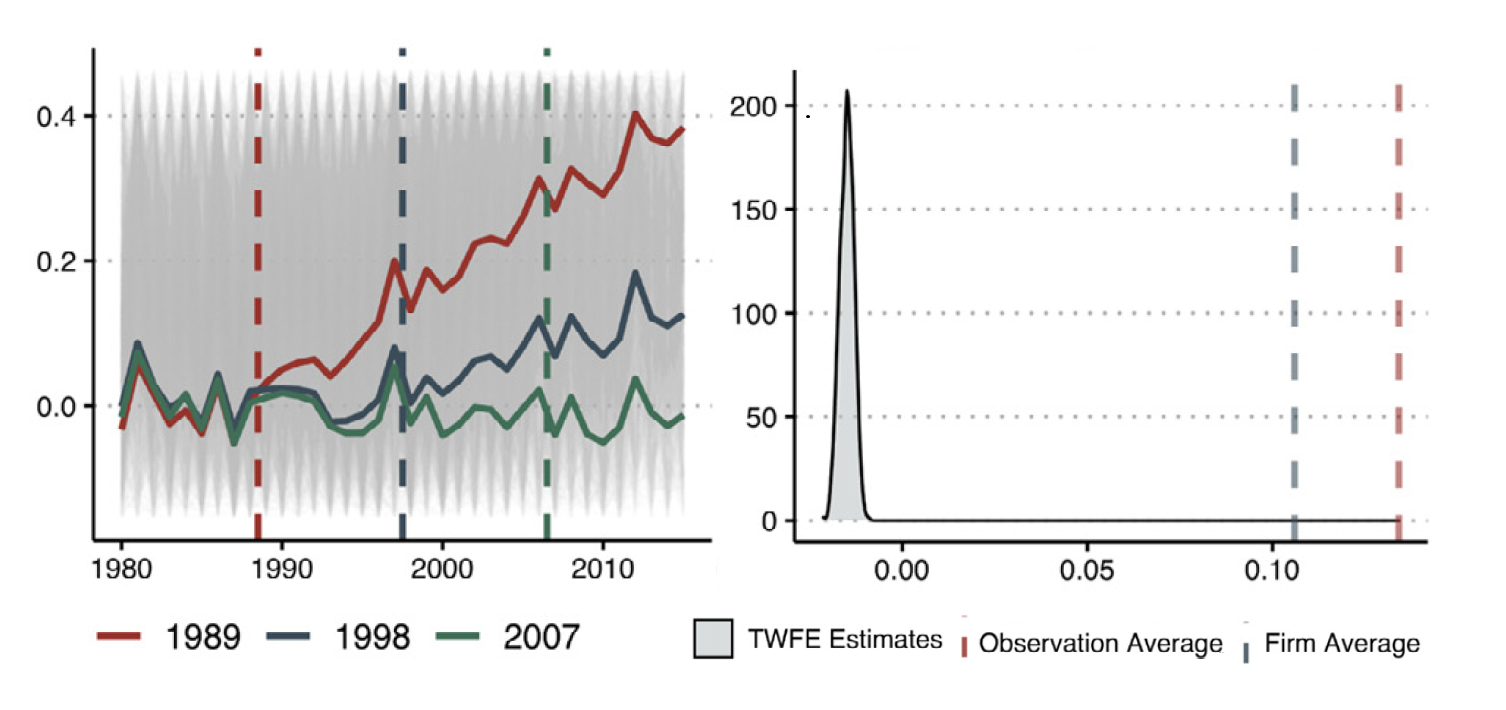
\includegraphics[width=6in]{Figures/Baker et al. (2022) Figure 2.png}
    \label{fig:baker-fig2}
\end{figure}
\noindent \citet{sunabr2021a} extend Prof. Goodman-Bacon’s result to dynamic DiD models, which measure treatment effects over time rather than a single average. They show that dynamic models suffer from the same weighting and forbidden comparison issues as the single DiD coefficient. Their results also cast doubt on the validity of common parallel trends tests, which we discuss below.\footnote{See also, \citet{roth2023s}, p. 2233}  This is a consequence of the negative weights underlying the dynamic DiD coefficients.

Other papers have confirmed the unexpected results hidden within DiD coefficients in staggered settings and helped advance our theoretical knowledge. For example, \citet{CS2021} carefully explain how the not-yet-treated group that forms as a consequence of staggered treatment can be incorporated into DiD analysis, as well as discussing how covariates affect interpretation of treatment effects. \citet{de2020two} decompose the TWFE coefficient similarly to Goodman-Bacon and provide additional intuition on the negative weighting problem. \citet{borusyak2024revisiting} show that unbiased treatment effect estimates can be recovered under a standard regression-based imputation procedure, while also advancing the mathematical rigor of DiD estimation under more general conditions. \citet{wooldridge2021two} establishes the equivalence of TWFE-type models with Mundlak estimators and pushes the limits of flexible interaction between treatment effects and covariates.

The general consensus from the literature is: if the policy has a heterogeneous effect on the affected units, and/or the policy effect changes over time, then TWFE and other classical DiD models are ill-equipped to handle proper estimation.

Along with diagnosing the forbidden comparisons problem with staggered treatment and heterogeneity-masking effects of TWFE models, the new literature has proposed a swathe of alternative models and sensitivity tests that address the issues. The general solution is straightforward: \textbf{eliminate the forbidden comparisons from your DiD estimation}. There are a variety of ways to do this. You can run separate regressions for each 2x2 DiD model with manually altered control groups, or combine each “cleaned” dataset into a “stacked” dataset without the forbidden comparisons and run a combined model. You can calculate potential untreated outcomes with TWFE in a first step and then compare treated outcomes to the predictions (so-called “imputation” estimators). You can turn to non-OLS estimation strategies like machine learning or maximum likelihood techniques. Lastly, researchers have devised modified linear regressions that automatically remove forbidden comparisons (so-called Extended TWFE or ETWFE models).  Each method has strengths and weaknesses, as we discuss below. Ultimately, while different methods of estimation should be used to ensure robustness, we prefer the ETWFE estimators from Sun and Abraham and Wooldridge, and the imputation frameworks of Gardner and Borusyak et al.  Requiring no data manipulation or exotic techniques, these methods rely only on linear regressions, making them easier to explain and interpret.

As a result of the seminal papers of Goodman-Bacon, Sun and Abraham, Wooldridge, Callaway and Sant’Anna, Borusyak et al., de Chaisemartin and d’Haultfoeuille, among others, there has been an influx of new papers on DiD theory. A simple search for DiD-related terms finds over 180 papers concerning DiD theory since 2018.\footnote{\url{https://arxiv.org/search/advanced?advanced=&terms-0-term=\%22difference-in-difference\%22&terms-0-operator=AND&terms-0-field=abstract&terms-1-term=\%22diff-in-diff\%22&terms-1-operator=OR&terms-1-field=abstract&terms-2-term=TWFE&terms-2-operator=OR&terms-2-field=abstract&terms-3-term=\%22two+way+fixed+effects\%22&terms-3-operator=OR&terms-3-field=abstract&classification-economics=y&classification-physics_archives=all&classification-include_cross_list=include&date-filter_by=date_range&date-year=&date-from_date=2018&date-to_date=2024-02-20&date-date_type=submitted_date&abstracts=hide&size=200&order=-submitted_date} (last accessed February 20, 2024).}  Prof. Goodman-Bacon’s work is currently cited by approximately 5,000 papers.\footnote{\url{https://scholar.google.com/scholar?cites=604067916365634144&as_sdt=20005&sciodt=0,9&hl=en} (last accessed February 20, 2024).}

This new DiD literature has already become a lecture topic in current PhD-level econometrics courses.\footnote{\url{https://donskerclass.github.io/files/pdf/CausalEconometricsSyllabus.pdf} as of March 12, 2024.}  It has also been the subject of several conferences and seminars in the past few years,\footnote{Some examples include: UCLA, “Difference-In-Difference Panel Discussion and Mini Conference” in May 2023; YoungStatS, “Advances in Difference-in-Differences in Econometrics” on December 15, 2021, presented; Mixtape Sessions, “Advanced Difference-in-Differences” seminar on April 21, 2023; Northwestern University, “Advanced Causal Inference Workshop” on August 13-17, 2023; Emory University, “Causal Inference Using Difference in Differences” on November 10, 2023.} as well as special journal issues.\footnote{The Econometrics Journal “Virtual Issue: The Econometrics of Treatment Effects.” \url{https://academic.oup.com/ectj/pages/treatment-effects-vi as of March 14, 2024.}} The new literature is also entering antitrust expert analysis as well. The authors have personally encountered some of the new papers in antitrust expert testimony, including the Callaway and Sant’Anna and Goodman-Bacon papers.

\section{Robust Analysis with Staggered Treatment} \label{sec:equations}

\begin{singlespace*}
\quote{
\textit{“One of the important conclusions is that there is nothing inherently wrong with TWFE as an estimation method. The problem is that it is often applied to a model that is too restrictive.”}
}\footnote{\citet{wooldridge2021two}, p. 34.}
\end{singlespace*}
\noindent We now discuss the form and implementation of some of the existing and new methods and sensitivities from the literature.
\subsection{Existing DiD Estimators}
The most basic DiD regression only uses 3 indicator variables: “treated,” which is 1 for affected units and 0 for control group units, “post” which is 1 after the start of the policy and 0 otherwise, and “post-treated,” which is the interaction of the two. The coefficient on “post-treated” is the measured DiD effect.
\begin{equation}
    y_{it} = \gamma \cdot \text{PostTreated}_{it} + \alpha\cdot \text{Treated}_i + \beta \cdot \text{Post}_t + \epsilon_{it}
\end{equation}
The basic TWFE model replaces “treated” with a set of unit fixed effects, and “post” with a set of time fixed effects:\footnote{Many other variations of TWFE and basic DiD models exist. For example, one might replace time fixed effects with covariates that appropriately control for variation over time. Polynomial terms might be included to account for non-linear relationships. Other models may add time-trend interactions to capture changing covariate relationships over time.}
\begin{equation}
    y_{it} = \gamma D_{it} + \alpha_i + \lambda_t + \beta X_{it} + \epsilon_{it},    
\end{equation}
Where one controls for agents, $\alpha_i$, time, $\lambda_t$, and optional control variables $X$. The coefficient of interest is $\gamma$ which quantifies the effect of the policy. “$D$” in the equation is the same as “PostTreated” in the previous equation. Researchers typically report standard errors clustered at the unit level to account for potential serial correlation.\footnote{For further reading, see \citet{bertrand2004}.} 

The dynamic TWFE model then interacts the treatment effect with relative-time indicators (i.e. time before/after starting treatment). Note that there are now several treatment effects being measured, one for each relative time period. This allows researchers to see if treatment effects change over time.
\begin{equation}
    y_{it} = \sum_{r=p}^R\left(\gamma_r\cdot\mathbbm{1}[t_r=r]\right) + \alpha_i + \lambda_t + \beta X_{it} + \epsilon_{it},    
\end{equation}
In this equation, “$t_r$” is relative time, i.e. the number of time periods before/after the start of treatment.\footnote{An example would be an indicator for relative time = -2, which equals 1 for observations 2 time periods before starting treatment.} Some researchers include pre-exposure periods in the model.  Parallel trends and anticipation effects are commonly assessed by testing if pre-exposure coefficients are different from zero. In a staggered treatment design, relative times would average across several calendar periods. For example, “1 year after starting treatment” would be 2008 for units who start in 2007, and 2010 for those who start in 2009.
\subsection{New DiD Estimators}
\citet{sunabr2021a}’s estimator modifies the dynamic model to also estimate separate treatment effects by treatment cohort. A “cohort” is a group of units that start their treatment at the same time.\footnote{For example, states that changed their minimum wage in 2010 would be in a different cohort than states that changed in 2012.}  By saturating the model with separate treatment effects, their estimator removes the forbidden comparisons that could lead to bias in a standard DiD model.\footnote{As it is saturated, certain indicators are omitted to prevent collinearity. Researchers typically omit the indicators for one period before starting treatment. Also, when there are no never-treated units in the data, another set of indicators must be removed, typically the last set of time indicators.}  Note that the authors did not examine how adding covariates to the model would affect results. Like the typical dynamic TWFE model, the policy effect is estimated with respect to how long units have been subjected to the treatment. Unlike the dynamic TWFE model, however, Sun and Abraham’s model additionally measures how units that start their treatment earlier in time differ from those who start their treatment later.
\begin{equation}
    y_{it} = \sum_{v=c}^C\sum_{p=r}^R\left(\gamma_{vp}\cdot\mathbbm{1}[t_r=p]\cdot \mathbbm{1}[\text{cohort}_i=v]\right) + \alpha_i + \lambda_t + \epsilon_{it},
\end{equation}
The \citet{wooldridge2021two} estimator is essentially an extension of the Sun and Abraham method.\footnote{Prof. Wooldridge offers two equivalent ways of estimating cohort-specific treatment effects: regular TWFE-style models, and Mundlak-style estimators which include group averages. For simplicity, we show the TWFE-style approach.}  The Wooldridge model not only measures treatment effects by cohort and over time, but it also allows for the treatment effect to vary with respect to covariates.\footnote{Prof. Wooldridge and other papers tend to focus on time-invariant control variables; these are seen as “safer” to include in DiD analysis because it’s less likely that the controls would affect treatment status and vice versa. Special care must be given to time-varying covariates to ensure their exogeneity to the treatment effect. For new research on interpreting DiD effects with time-varying controls, see \citet{caetano2023} and \citet{wooldridge2023nonlinear}, C60 (Section 7.3).} Besides allowing more flexibility in the model, an advantage of this framework is that the parallel trends assumption becomes more realistic: control and treatment units would move similarly over time after controlling for observed covariates in the absence of the treatment effect. With $L$ covariates, and using $\dot{x}$ to represent cohort-demeaned controls, the model is:\footnote{This is Prof. Wooldridge’s equation 6.33 on p. 44. The average marginal effect of treatment with this method is equivalent to Stata’s \texttt{xthdidregress twfe} command with unit-level clustered errors. As explained in the paper, demeaning $x$ by cohort is not necessary for correct treatment effect estimation, but it makes interpreting the other coefficients easier.}
\begin{multline}
    y_{it} = \sum_{v=c}^C\sum_{q=t}^T\left(\gamma_{vq}\cdot\mathbbm{1}[t=q]\cdot \mathbbm{1}[\text{cohort}_i=v]\right) + \alpha_i + \lambda_t \\
    + \sum_{x=k}^L\sum_{v=c}^C\sum_{q=t}^T\left(\theta_{vq}\cdot \mathbbm{1}[t=q]\cdot \mathbbm{1}[\text{cohort}_i=v] \cdot \dot{x}_{itk}\right) + \alpha_i X_{it} + \lambda_t X_{it} + \beta X_{it} +\epsilon_{it},
\end{multline}
Note that the first part of the equation is like the Sun and Abraham estimator, while the rest of the equation incorporates flexible treatment interaction with the covariates.\footnote{The Sun and Abraham model is in terms of relative time, while the Wooldridge model uses calendar time. This leads to slightly different notation and interpretation of coefficients, but the estimated effects are the same.}  The additional terms include a set of cohort-time interactions for each covariate, a full set of unit indicators for each covariate, a full set of time indicators for each covariate, and the covariates themselves. Prof. Wooldridge explains how to aggregate these treatment effect estimates and adjust their standard errors for sampling variation in the covariates, which may provide more conservative inference than other new estimators.\footnote{\citet{wooldridge2021two}, pp. 32-33.}

The \citet{borusyak2024revisiting} and \citet{gardner2022a} estimators both use an imputation approach, in which the appropriate unit and time effects are estimated from a regression on untreated observations, and then a second step determines the policy effect. The Borusyak et al. procedure works by regressing on fixed effects for untreated observations only (denoted by the “0” superscript), then predicting these effects onto the treated observations and forming an observation-specific treatment effect estimate. The results from the first step (denoted $\Hat{y}_{it}^0$ ) represent the model’s prediction of treatment unit outcomes in absence of the treatment effect.
\begin{align}
    1. \quad & y_{it}^0 = \alpha_i + \lambda_t + \epsilon_{it} \\
    2. \quad & \gamma_{it} = y_{it} - \Hat{y}_{it}^0
\end{align}
Researchers can then aggregate the treatment effect estimates as needed.

The Gardner method is similar but automatically aggregates the estimated effect. After running the first step (regression on untreated observations), a second step regresses adjusted outcomes on treatment status:
\begin{equation}
(y_{it} - \Hat{y}_{it}^0) = \gamma D_{it} + \epsilon_{it}    
\end{equation}
Both papers discuss how covariates can be incorporated into the model and how treatment effects can be estimated over time, by cohort, or just a single average effect.

Calculating standard errors for imputation treatment effects is different from the ETWFE methods, since researchers must account for variation coming from both estimation steps. Borusyak et al. recommend a conservative inference method which carries over regression residuals from step 1.\footnote{\citet{borusyak2024revisiting}, pp. 19-21 (Theorem 3).}  Prof. Gardner instead shows how his 2 regressions can be estimated simultaneously using GMM.\footnote{\citet{gardner2022a}, pp. 12-13.}
\subsection{Discussion}
The techniques we discussed can account for additional treatment effect heterogeneity if needed. For example, in a price-fixing conspiracy of differentiated products, certain groups of products may be more affected by the conspiracy than others, due to varying local competition or other product-specific factors. In this case, estimating single coefficients for each cohort and time period gives a weighted average of the true effects. Practitioners can easily modify the above equations to additionally measure a treatment effect for each product group, but this may make the model computationally difficult to run with flexible models. This type of heterogeneity does not introduce forbidden comparisons in the model, but separate estimation allows researchers to choose a more appropriate weighted average than what the model would select otherwise.

While its flexibility can be beneficial, the full Wooldridge regression will include an extremely large number of variables if there are many treatment cohorts and covariates.\footnote{The number of variables in the regression grows approximately on the order of (number of cohorts squared) times (number of covariates). After partialling out the fixed effects, a TWFE implementation includes $1 + n(Q-q+T+1) + (n+1) \sum_{i=q}^Q(T+1-i)$ variables, where $n$ is the number of covariates, $T$ is the number of time periods, $q$ is the time of the first cohort, and $Q$ is the time of the last cohort. This assumes that units become treated in each time between $q$ and $Q$ and each cohort stays treated through the end of the data. For example, with 2 covariates, 20 time periods, and treatment cohorts between times 10 and 15, the regression would have 206 variables vs just 4 in a standard TWFE model.}  Besides running very slowly or not at all, Wooldridge-type models may lack precision by estimating so many effects.\footnote{See \citet{faletto2023a} for a regularization approach to gain estimator efficiency in the presence of sparsity among the Wooldridge controls. But this technique does not reduce the (potentially infeasibly large) time needed to run such regressions. Future research might look into pre-regression dimensionality reduction as a method to combine and reduce the number of variables feeding into ETWFE-type models.}  With a priori knowledge, practitioners can reduce the variable count by restricting treatment patterns.\footnote{For example, if you believe that the treatment effect is constant over time, you can remove the time-specific treatment effects from the equation and only allow for cohort-specific effects.}  Binning variables is another common choice for practitioners to reduce variable count, in which (for example) treatment effects in monthly data would be measured by quarterly or yearly treatment effects. However, this is not without potential issue, as discussed in \citet{borusyak2024revisiting} Section 5.2.1 and Figure 3. They find that DiD analysis from \citet{broda2014} changed dramatically when removing the binning technique, and Borusyak et al. conclude that monthly binning of weekly data imposed a “short-term bias” on the results, where positive weights are given to earlier weeks in the month, and negative weights are given to the last week in each month. Borusyak et al. and Sun and Abraham provide strategies to estimate these weights using the Frisch-Waugh-Lovell theorem (essentially an auxiliary regression of treatment status on fixed effects);\footnote{\citet{borusyak2024revisiting}, Appendix A15 (Proof of Proposition 2). \citet{sunabr2021a}, p. 181 (Equation 13)}  researchers that are binning should run these regressions as sensitivities to assess potential short-term bias in their models.

In the ETWFE models, practitioners often want to report a single coefficient, or one coefficient per calendar period. Sun and Abraham explain that it is easy to aggregate the coefficients after estimation; one can simply use sample probabilities for each cohort-period, or alternatively weight the probabilities by revenue or volume for damages analysis if the evidence suggests doing so.\footnote{\citet{sunabr2021a}, p. 186 (Section 4.1, Step 3). See also \citet{borusyak2024revisiting}, p. 16 (Theorem 2, Step 3).}  In any case, these methods circumvent the main problem with the original DiD models: they all eliminate the forbidden comparisons and provide control over what weighted average of treatment effects is being calculated.
\\
\textbf{Sensitivities}: While we have described some possible sensitivities for expert analysis work so far, we provide a more comprehensive list in  \hyperref[sec:appendixa]{Appendix A} below.
\section{Special Considerations for Antitrust Practitioners} \label{sec:antitrust}
We now discuss three topics that we consider particularly important for antitrust analysis: parallel trends assumptions, the not-yet-treated group, and unbalanced panels. Then in  \hyperref[sec:analysis]{Section V}, we investigate some related properties of staggered DiD in a Monte Carlo analysis.
\subsection{Cautions on Parallel Trends} \label{sec:parallel-trends}
The new literature has shown that common parallel trends tests can suffer from bias in the presence of heterogeneity. Additionally, while several new estimators have been proposed for testing parallel trends in the presence of heterogeneous effects, recent research shows that visual examination of coefficients is not a reliable assessment for many of the new estimators.\footnote{\citet{roth2024a}, p. 7 (“The first practical takeaway from these results is that the default event-studies from CS, dCDH, and BJS should not be interpreted in the same way as traditional dynamic TWFE event-study plots. … One should therefore not apply the typical heuristics for visual inference—e.g. looking for a discontinuity or kink at the treatment date—that may be familiar from TWFE event-studies in the non-staggered case.”).}  Antitrust practitioners arguing either for or against parallel trends in a DiD model should follow guidance from the new literature. In both cases, expert opinion should be supported with analysis demonstrating (lack of) \textit{economically} significant differences between the treatment and control groups, not just statistically significant results.

Conventional parallel trends test results should always be taken with caution. \citet{roth2023s} summarize many issues with testing for parallel trends brought up in recent years. First, based on how they are conducted, the tests can suffer from low power in smaller datasets.\footnote{\citet{roth2023s}, p. 2233.}  Second, selecting models based on what “passes” the parallel trends test induces testing bias.\footnote{See \citet{roth2022a} for an in-depth discussion of such biases and practical considerations.}  Third, in large datasets, it is very likely that the parallel trends testing coefficients will be statistically significant. This is true for most DiD models in antitrust analysis with microdata, in our experience. But the magnitude of the violation is more important. Practitioners should try to size the potential bias of observed parallel trends issues, rather than simply rejecting the usefulness of DiD in general. 

\citet{rambachan2023more} (discussed in \citet{roth2023s}) pose a framing question: How large would the bias from unparallel trends have to be to make the resulting treatment effect statistically insignificant?\footnote{\citet{rambachan2023more} at Section 6.2. \citet{roth2023s} at section 4.5 (“one type of restriction [Rambachan and Roth] consider states that the magnitude of the post-treatment violation of parallel trends can be no larger than a constant M times the maximal pre-treatment violation. … This indicates that to invalidate the conclusion of a positive effect, we would need to allow for a post-treatment violation of parallel trends [M] times larger than the maximal pretreatment violation.”).}  Several sensitivities follow from this question, ranging from visual inspection to alternative model specifications.\footnote{See \hyperref[sec:appendixa]{our Sensitivities Appendix below} for more detail.}  This framework is of particular interest for antitrust impact analysis, where bias from lack of parallel trends can make or break an expert’s conclusion or lead to \textit{Daubert} exclusion. Similar to a confidence interval, experts should know how far the parallel trends assumption can be bent until their model breaks. Importantly, the literature seems to point to the conclusion that a statistically significant (but economically insignificant) difference in parallel trends, particularly in large datasets, is not a fully reliable measure to invalidate DiD results.

An additional caution on parallel trends comes when covariates are added to the regression. While adding covariates can make the parallel trends assumption more realistic (trends in outcomes are parallel \textit{after conditioning on covariates}), DiD models implicitly assume that any covariates are exogenous to the policy effect, and/or that covariates enter linearly into the conditional mean function. Failing those assumptions will bias your results in an unknown direction, and the new estimators are not robust to these types of misspecification. The flexible Wooldridge model discussed above allows policy effects to vary by covariates, but still assumes that the treatment effect does not influence the covariates. Practitioners should weigh the benefits of including covariates with the risk of bias from endogeneity in their models.

Finally, the presence of two groups of effective controls (never-treated and not-yet-treated) means that parallel trends could hold for one (or both) of these groups. Some papers have defined separate parallel trends assumptions for each group (Callaway and Sant’Anna), while others treat them the same (Borusyak,  Gardner).\footnote{\citet{CS2021}, p. 204 (Assumptions 4 and 5). \citet{borusyak2024revisiting}, p. 8 (Assumption 1). \citet{gardner2022a}, Equation 1.}  Researchers should consider which of these groups is more likely to satisfy parallel trends based on context. But in practice, the assumption is often based on data availability.\footnote{\citet{CS2021}, p. 205.}  We recommend running three types of models if data is available: one using the never-treated group, one with the not-yet-treated group, and one using both groups. Substantially different results from these models may indicate a compositional difference between the two control groups and may be worth exploring. Additionally, many of the new estimators in the literature allow you to specify which group you want to use as a control, though they tend to default to the never-treated group.

In any case, we think that the new literature has weakened the assurance of postestimation parallel trends tests. If you are not sure that the regression is correctly specified, parallel trends tests may provide an opposite conclusion to the truth. If you have small or noisy data, your test may be underpowered. If you have large data, your test may reject parallel trends but with an economically insignificant effect to the results. In expert testimony, work in support of a DiD analysis should put more effort into providing sensitivities such as in Rambachan and Roth’s “what-if” analysis, as well as giving theoretical justification of approximately conditional parallel trends. Work against DiD analysis should not rest on a statistically significant postestimation parallel trends test as a complete invalidation of a model; instead, practitioners should demonstrate that the resulting bias is economically meaningful. This could mean showing that damages disappear under a model which corrects for uncommon trends, or that the but-for predictions of the model are substantially different from reality.
\subsection{Not-Yet-Treated Group as a Source of Identification}
A consequence of staggered treatment designs is that at certain times, some units are currently experiencing the treatment, while others will be treated, but haven’t started their treatment yet (the “not-yet-treated group”). Others still may never experience the treatment (the “never-treated group”). The not-yet-treated group does not exist in a common-timing treatment design. However, the not-yet-treated group offers both benefits and potential drawbacks to applied researchers.

Classical DiD models require a control group of units that have never experienced the treatment. In staggered models, however, the not-yet-treated group can be used as an effective control group under the right conditions. In fact, the not-yet-treated group is in some cases a better control than the never-treated group, if one is worried that groups that eventually receive the treatment are uncontrollably different from groups that never receive it.

The not-yet-treated DiD model is also different from a standard before-after regression. This is because while the before-after model (with one treatment time) has no unaffected units after the start of treatment, in a staggered setting, the data allow a contemporaneous effective control group for all cohorts except the very last one.\footnote{This is because if all cohorts eventually become treated, then there cannot be untreated units by the last time period. Some papers suggest removing the last period of data from the model to treat the last cohort as a “never-treated” group. \citet{wooldridge2021two}, p. 52.}  For example, by the time cohort 1 becomes treated, cohort 2 has not been treated yet, so at time 1, it is a control group for cohort 1. Similarly, cohort 3 is a control for cohort 2 at time 2, and so on. We just need to be careful in setting up the DiD model to not allow for the forbidden comparisons inherent in the single coefficient model.

As we discussed in Section \ref{sec:literature} above, negative weights arise because the TWFE DiD estimate includes already-treated units as part of the control group.  Because of this, units that begin their treatment early in the data are more likely to suffer from negative weights. While this issue occurs whether you include the not-yet-treated group or not, removing the group could increase the negative weight bias by removing correct component DiDs from the weighted average TWFE effect. Also, with more treatment cohorts, already-treated units will be used as effective controls more often. Antitrust practitioners should keep this in mind when examining a TWFE model. Early-treated units have the highest risk of negative weights neutralizing their treatment effect. In the case of a price-fixing conspiracy that dissolves over time due to cheating, the price-increasing effects may be concentrated within earlier treatment cohorts. A naïve TWFE model could substantially bias the estimated effect in this scenario.
\subsection{Unbalanced Panels and the Always-Treated Group}
It is often the case that units (e.g. customers, suppliers, stores) are not present for the entire period of the data. In practice, units can enter into the analysis or exit in two ways. First, units can be partially present in the data because of a sampling issue. Second, units can be present in the data because they truly enter or exit in the period of the analysis (i.e. with no sampling issue). While the first type of partial presence is an important issue in itself, we focus on the second situation. Entry and exit within a staggered treatment design brings additional sources of concern for DiD analysis.

In panel data, if units are missing for some periods, then it is called an unbalanced panel (as opposed to a balanced panel). General theories related to dealing with unbalanced panel data are beyond the scope of this paper.\footnote{See generally, \citet{wooldridge2010a}, Chapter 17 (“Sample Selection, Attrition, and Stratified Sampling”) and \citet{cameron2020}, Chapter 27 (“Missing Data and Imputation”).}  However, we highlight a special case where a unit is not present either before or after the policy implementation in a DiD analysis. This situation happens regularly in our experience with staggered DiD antitrust analysis. For example, a store may open in the midst of a price-fixing conspiracy affecting other local stores. In this example, the store has no “before” period to compare to in a typical DiD scenario; it is part of the always-treated group.
\begin{figure}[H]
    \centering
    \caption{Example of Unbalanced Panel with Staggered Treatment}
    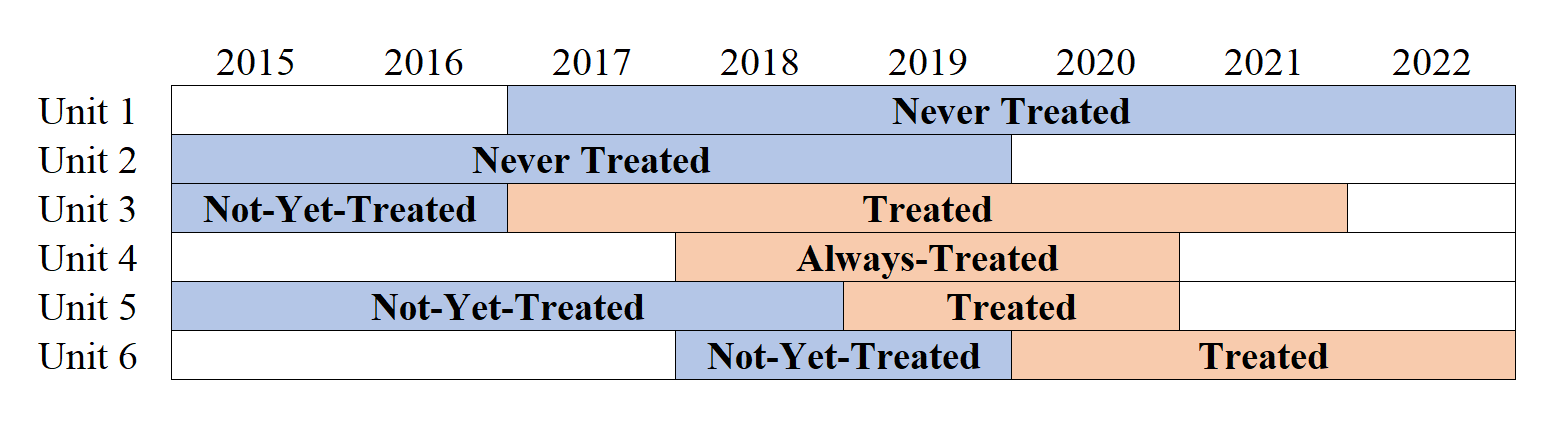
\includegraphics[width=6in]{Figures/Visual Staggered Unbalanced Treatment.PNG}
    \vspace{2mm}
    \footnotesize \begin{singlespace*}
        \parbox{5.5in}{Example of a staggered treatment mechanism with unbalanced data. Unit 4 has no “before” period and so is part of the always-treated group.}
    \end{singlespace*}
    \label{fig:visual-unbalanced}
\end{figure}
\noindent In a staggered TWFE or similar DiD model, the always-treated group will be automatically included in the analysis (it is not removed from the regression). But the model implicitly assumes that the policy effect on those units is similar to the average effect of the policy on units that are present (even partially) before and after the start of the policy. In contrast, if the treatment effect is different for always-treated units (for example because they tend to appear later in the data and the treatment effect is dynamic), then omitting them would change the estimated effect in a TWFE model. We recommend running the regression both with and without them to quantify their importance to the treatment effect. Our experience is that the group tends to make little to no difference to the estimated DiD effect. However, the new DiD methods do not suffer from this type of bias.

When utilizing the always-treated group, antitrust practitioners must justify the assumption of similarity with the other treated units. In some scenarios, it may make sense that treatment effects are different for the always-treated units. For example, a cartel may find more leverage in overpricing new customers than customers that existed before the conspiracy (who are familiar with competitive prices). On the other hand, it’s also possible that a cartel could lure in new customers with competitive prices, then increase the prices later. The DiD estimators we discuss would correctly capture this effect only if the cartel ramps up the new customers’ prices in the same way as for others in the same treatment cohort. Depending on case-specific context, it may be worthwhile to compare trends for always-treated units to other treated units within the same cohort, if data is available.

\citet{de2023two} identify risks associated with the always-treated group in terms of weights given to the single DiD coefficient: cohorts that are always treated are more likely to get negative weight in the TWFE averaging.\footnote{\citet{de2023two}, p. 5 (“Accordingly, all the weights are likely to be positive when there is no group that is treated most of the time, and no time periods where most groups are treated.”).}  This is mitigated by the many new estimators we have described above.

Some types of new estimators from the literature explicitly exclude always-treated units. Imputation-based estimators from \citet{borusyak2024revisiting} and \citet{gardner2022a} learn the fixed effects from a regression on untreated observations, then learn the treatment effect after partialling out the estimated fixed effects. If you use unit fixed effects, then you have no pre-treated data for always-treated units. Prof. Gardner hypothesizes that you could use treated observations in the first step, so long as you have a correctly specified conditional mean function,  but this requires justification.\footnote{\citet{gardner2022a}, note 8.}

\citet{borusyak2024revisiting} note that in unbalanced panels, if the composition of units within each cohort changes over time, then cohort-based estimators can be biased.\footnote{Cohort-based estimators are methods that include fixed effects at the treatment cohort (rather than unit) level. In balanced panels, cohort- and unit-based estimators are equivalent when standard errors are clustered at the unit level.}  This is because cohort-based estimators assume a constant composition within the cohort over time.\footnote{\citet{borusyak2024revisiting}, Appendix A2-A3 (“Our unit fixed-effects model can handle missing observations even when the composition of units changes over time, while cohort-based parallel trend assumptions (e.g. that $E[Y_{i,t+1}(0) - Y_{it}(0) | E_i]$ does not vary with $E_i$) may be unattractive; similarly, estimation with cohort, rather than individual, fixed effects can lead to biases with incomplete panels.”).}  The benefit of cohort-based estimators is that they can retain some of the data that would be dropped with unit-level estimators. With imputation estimators at the unit level, always-treated units have no untreated data for the first regression, and so those records fall out of the model.

In the Monte Carlo results we present in the next section, we report \hyperref[fig:estimators-balanced]{simulation results} which indicate that when the data is highly unbalanced, even the new DiD estimators can be subject to bias. However, they appear to converge to the correct value as data become more balanced, while TWFE generally will not.

\section{Monte Carlo Analysis} \label{sec:analysis}
\begin{singlespace*}
\quote{\textit{“When the adoption of the treatment by different groups is staggered over time, and the average effects of the treatment vary over groups and across time, the usual difference-in-differences regression specification does not identify a readily interpretable measure of the typical effect of the treatment.”}}\footnote{\citet{gardner2022a}, p. 1.}\end{singlespace*}
\subsection{Data Description}
We simulate data with the following setup. There are 1,000 units (customers) and 20 time periods. This analysis is with a balanced panel (no entry or exit). We create treatment cohorts starting at times 10 through 15. We then create 6 datasets with different treatment effects:
\begin{align*}
    \text{Effect 1} &= 5\cdot D_{it} \\
    \text{Effect 2} &= (5 + \text{cohort}_i - \overline{\text{cohort}})\cdot D_{it} \\
    \text{Effect 3} &= (5 + \text{exposure}_{it} - \overline{\text{exposure}})\cdot D_{it} \\
    \text{Effect 4} &= (5 + \text{cohortTime}_{it} - \overline{\text{cohortTime}})\cdot D_{it} \\
    \text{Effect 5} &= (5 - \text{exposure}_{it} + \overline{\text{exposure}})\cdot D_{it} \\
    \text{Effect 6} &= (5 - \text{cohortTime}_{it} + \overline{\text{cohortTime}})\cdot D_{it} \\
    \text{cohortTime} &= \text{cohort}_i + \frac{\text{cohort}_i-10}{5}\cdot \text{exposure}_{it}.\\
\end{align*}
These treatment effects allow us to identify how heterogeneous and/or dynamic effects factor into the DiD estimators. All effects are normalized so that the average treatment effect on the treated (ATT) is equal to 5.

We then add unit and time effects and two standard normal variables, one for our noise parameter and one as a covariate:
\begin{equation}
     y_{it} = \alpha_i + \lambda_t + x_{it} + \text{Effect}_{it} \cdot D_{it} + \epsilon_{it},
\end{equation}
Shown below are the true treatment effects by cohort for the 6 treatment effects. They capture varying behaviors that would complicate a standard DiD analysis.
\begin{figure}[H]
    \centering
    \caption{Treatment Effects in Simulated Data}
    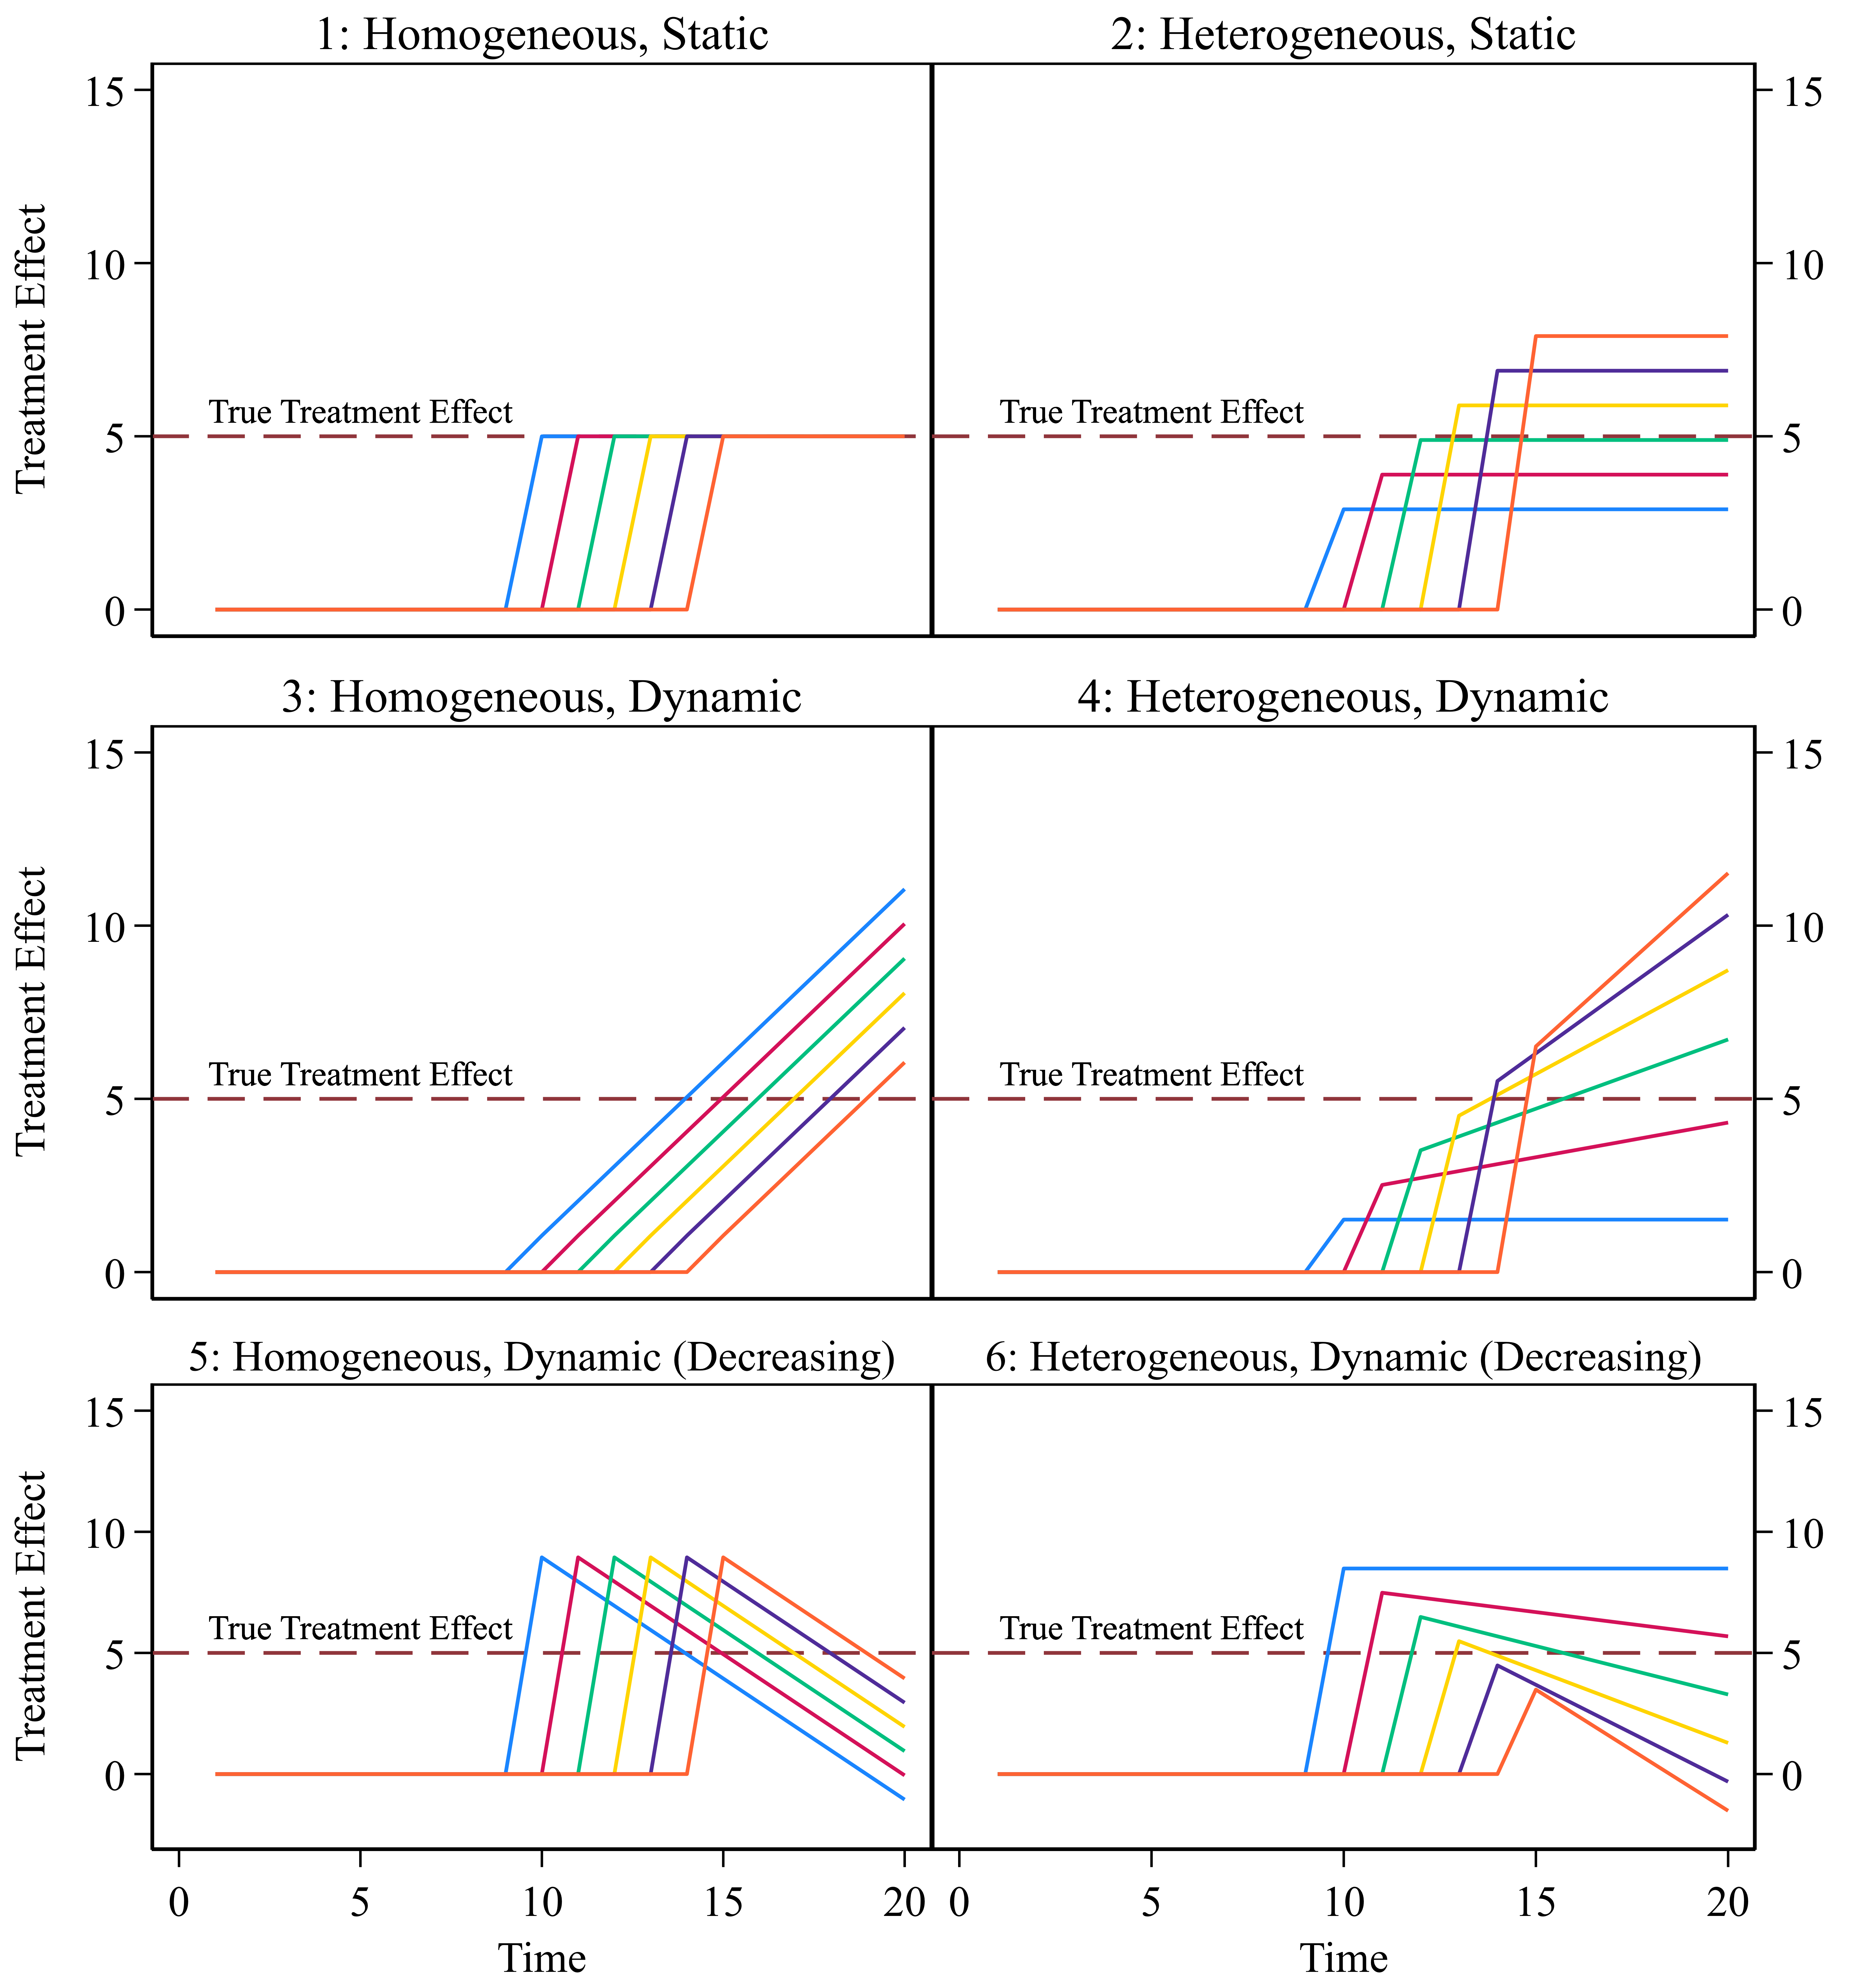
\includegraphics[width=6in]{Figures/Table 1 Treatment Effects Chart.png}
    \label{fig:treat-effects}
\end{figure}
\subsection{Results}
\subsubsection{Comparing Estimators with Never-Treated Control Group}
In Table \ref{tab:estimators-never}, we compare the finite-sample performance of several estimators under the 6 different scenarios described above. Our Monte Carlo exercise uses 1,000 randomly generated datasets with the 6 different effects, and the reported results are averaged across the simulations.\footnote{Distributions of our Monte Carlo estimators are reported in \hyperref[sec:appendixb]{Appendix B} below. Each regression model is run on each dataset 1,000 times.}

First, we can see that the TWFE results are biased (significantly different from the true effect) in all but the first dataset; this is consistent with the finding that TWFE is biased unless the treatment effect is homogeneous and static. Datasets 5 and 6 confirm that the direction of the staggered DiD bias depends on whether earlier treatment cohorts have higher (or lower) effects than later cohorts.\footnote{For example, in dataset 3, the earliest treatment cohort has the highest treatment effect over time, while the opposite is true for dataset 5. Since earlier-treated cohorts suffer most from negative weights, the high treatment effect is muted by negative weights in dataset 3 (leading to negative bias), and vice versa for dataset 5.}  Note that the magnitude of bias is the same between 3 and 5 (or 4 and 6), but in opposite directions.

Second, we find that all other methods recover the correct ATT, but with varying precision. The Wooldridge, Gardner, and Borusyak et al. methods with the control variable included have the lowest standard errors, which agrees with the literature.\footnote{Prof. Wooldridge establishes equivalence between his method and the Borusyak imputation, and both papers establish BLUE-like properties of their estimators. \citet{borusyak2024revisiting}, p. 16 (Theorem 2). \citet{wooldridge2021two}, p. 6 “Moreover, because the POLS/ETWFE estimator is also equivalent to random effects with known (rather than estimated) transformation parameter, under the standard no serial correlation and homoskedasticity assumptions, the POLS estimator is best linear unbiased. Thus, this simpler estimator has the same efficiency as the comparable imputation estimator in BJS (2021).”}  The Callaway and Sant’Anna method produces significantly larger standard errors, but this approach may still be desirable for its conservative inference and robustness to additional types of misspecification. Finally, this table quantifies the effects of omitting a time-varying covariate from the regression; omitting this variable increases the resulting DiD effect standard error from each of the methods.

Our Monte Carlo analysis also confirms point equivalences between some of the estimators. For instance, the Callaway and Sant’Anna (no covariates) and Sun and Abraham estimators have identical point estimates in each of our 1,000 simulations, when using the never-treated group.\footnote{\citet{sunabr2021a}, p. 187 (“In particular, without covariates and for the case with never treated units, our approach coincides with Callaway and Sant’Anna (2020a).”).}  The Gardner and Borusyak et al. methods have identical point estimates. While the Wooldridge standard errors look identical to Gardner and Borusyak et al., the point estimates are slightly different.
\begin{table}[H]
    \centering
    \caption{Statistical Comparison of DiD Methods with True Average Effect
Comparing Treated with Never-Treated and Not-Yet-Treated}
    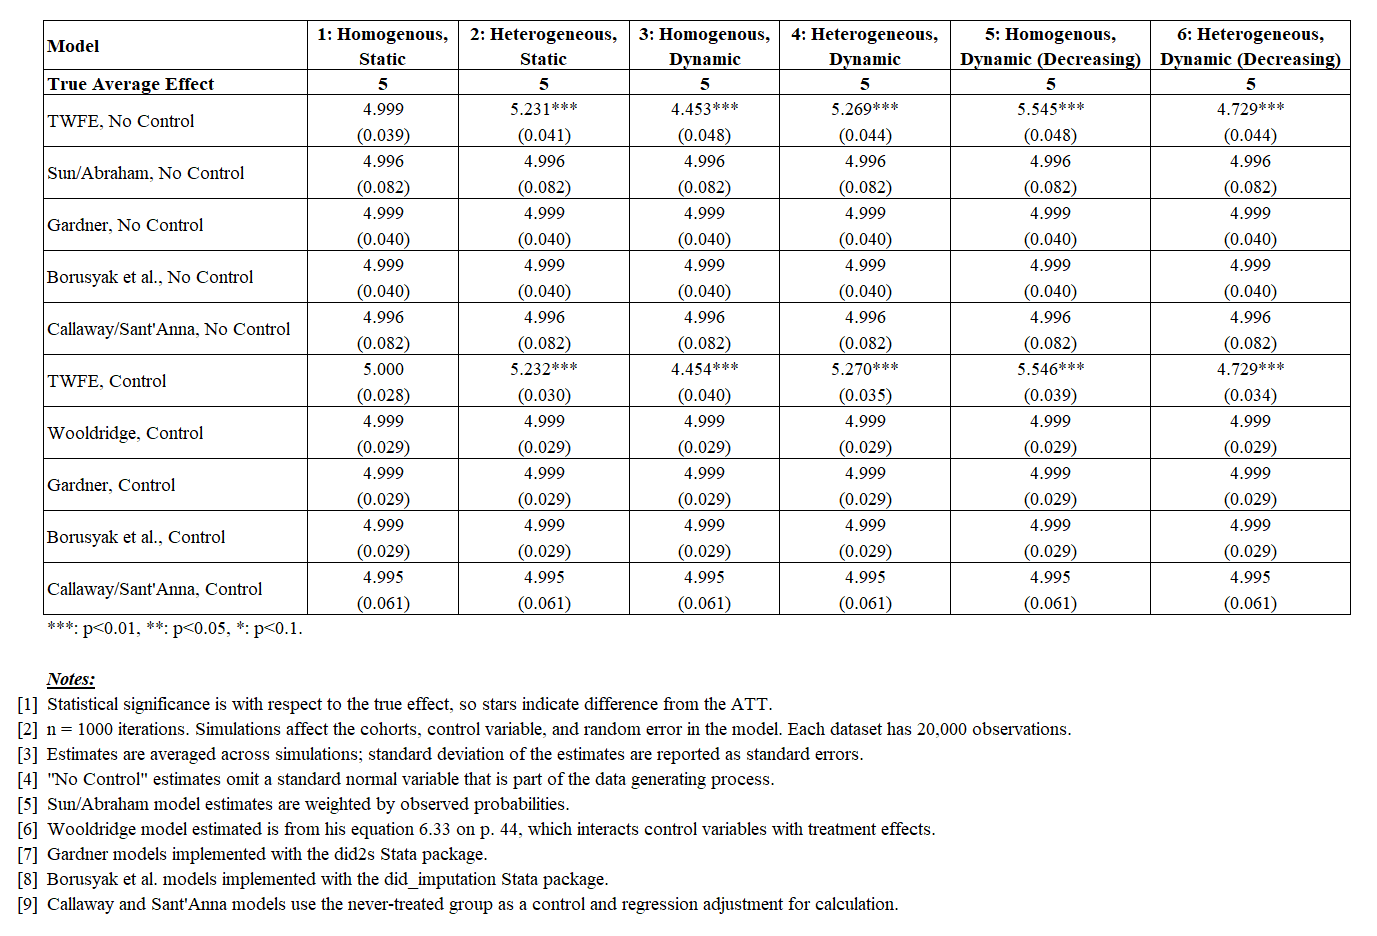
\includegraphics[width=6in]{Figures/Table 1.png}
    \label{tab:estimators-never}
\end{table}

\subsubsection{Comparing Estimators with Not-Yet-Treated Control Group}
Next, in Table \ref{tab:estimators-notyet}, we repeat the simulation exercise using only the not-yet-treated group as a control, meaning we remove the never-treated units. However, we cannot simply rerun the models with the remaining data. By time 15, all units are treated, which makes estimation of the treatment effect impossible for times 15 through 20. As a result, we also drop these time periods from the data.\footnote{Because these filters result in a substantially smaller dataset than the previous table, we increase the number of treated units so that the filtered data is approximately the same size as the original data.}  We rebalance the average treatment effect to remain at 5. 

Interestingly, when using the not-yet-treated group only, the TWFE estimates are only weakly different from the true effect under a heterogeneous, static treatment effect. The TWFE point estimates for dataset 2 are different from the other estimators, but substantially closer to the true effect when compared to the previous table. Further, while the Callaway and Sant’Anna (no covariates) and Sun and Abraham estimators were identical in the previous table, the Callaway and Sant’Anna estimator has lower standard errors here. Regardless, all of the new estimators continue to recover the true effect.
\begin{table}[H]
    \centering
    \caption{Statistical Comparison of DiD Methods with True Average Effect
Comparing Treated with Not-Yet-Treated Only}
    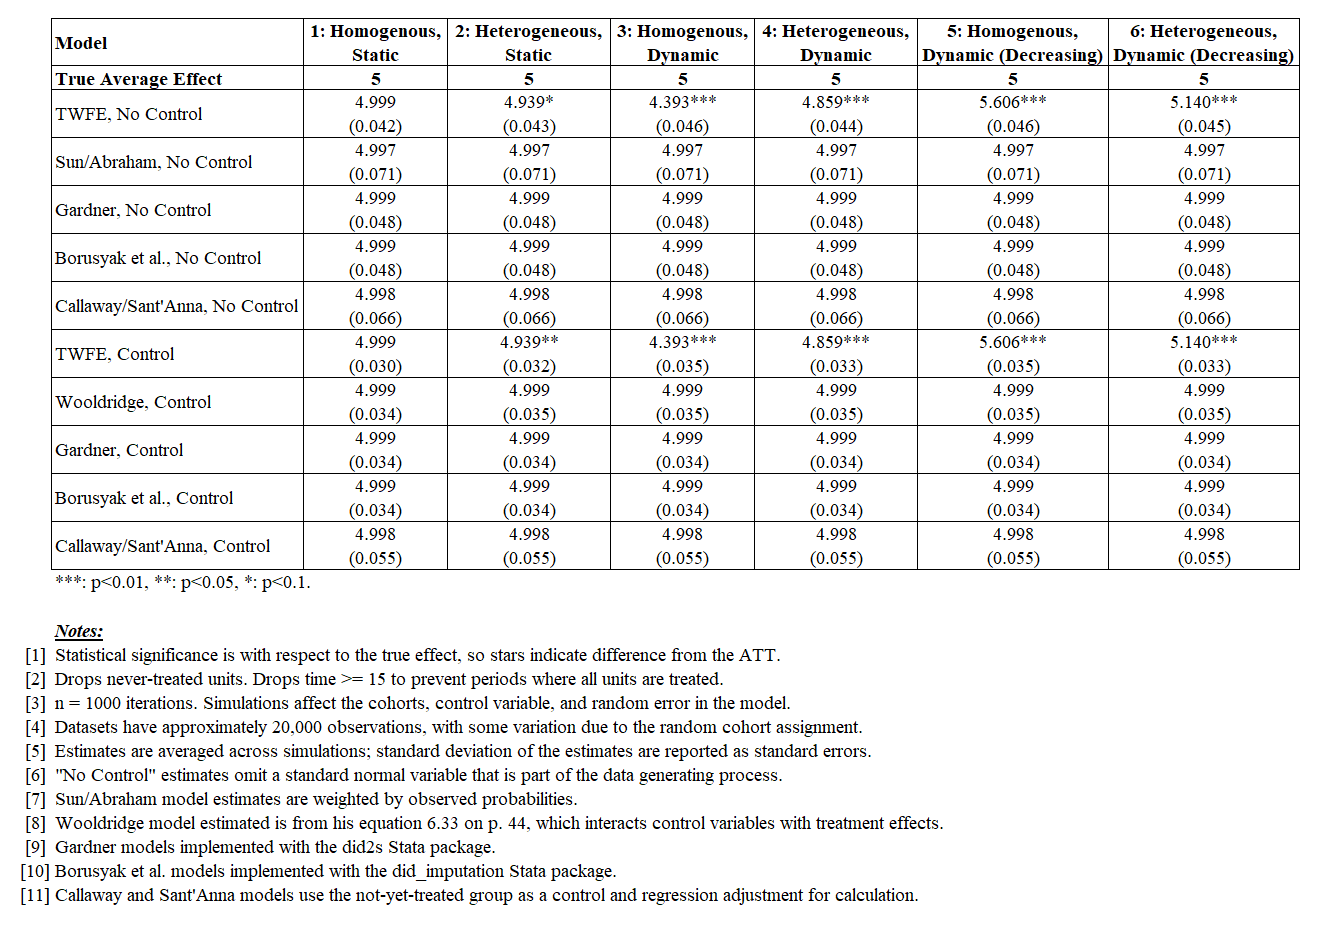
\includegraphics[width=6in]{Figures/Table 2.png}
    \label{tab:estimators-notyet}
\end{table}
\subsubsection{TWFE Bias by Composition of Control Group}
Next, we analyze how the composition of the control group varies the resulting TWFE bias. The horizontal axis in Figure \ref{fig:pc-nevertreat} below is the percentage of never-treated units in the control group; 0 means only not-yet-treated observations (no unaffected units), while 100 means only never-treated. The vertical axis is the  estimator bias (estimated effect minus true effect). As expected, when treatment effects are homogeneous and static, there is no bias regardless of never-treated composition. Next, the homogeneous and dynamic specification (the green line) has extreme bias when there are only not-yet-treated observations; the bias decreases quickly as we add never-treated units into the control group. The heterogeneous treatment effects (red and orange) are much less affected than the homogeneous dynamic effect (green). Interestingly, the bias from our heterogeneous and dynamic specification (orange) decreases until about 35\% never-treated, then increases as the percent of never-treated increases.

We also perform a sensitivity analysis to check if these (and other) findings are robust to alternative data specifications. We randomly varied the number of units, number of time periods, percent never-treated, first treatment time, last treatment time, percent balanced, treatment effect size and sign, individual-specific treatment heterogeneity, covariate effect size and sign, and covariate correlation with treatment status. See \hyperref[sec:appendixb]{Appendix B} for these additional results.
\begin{figure}[H]
    \centering
    \caption{TWFE Bias by Percent Never-Treated in the Data}
    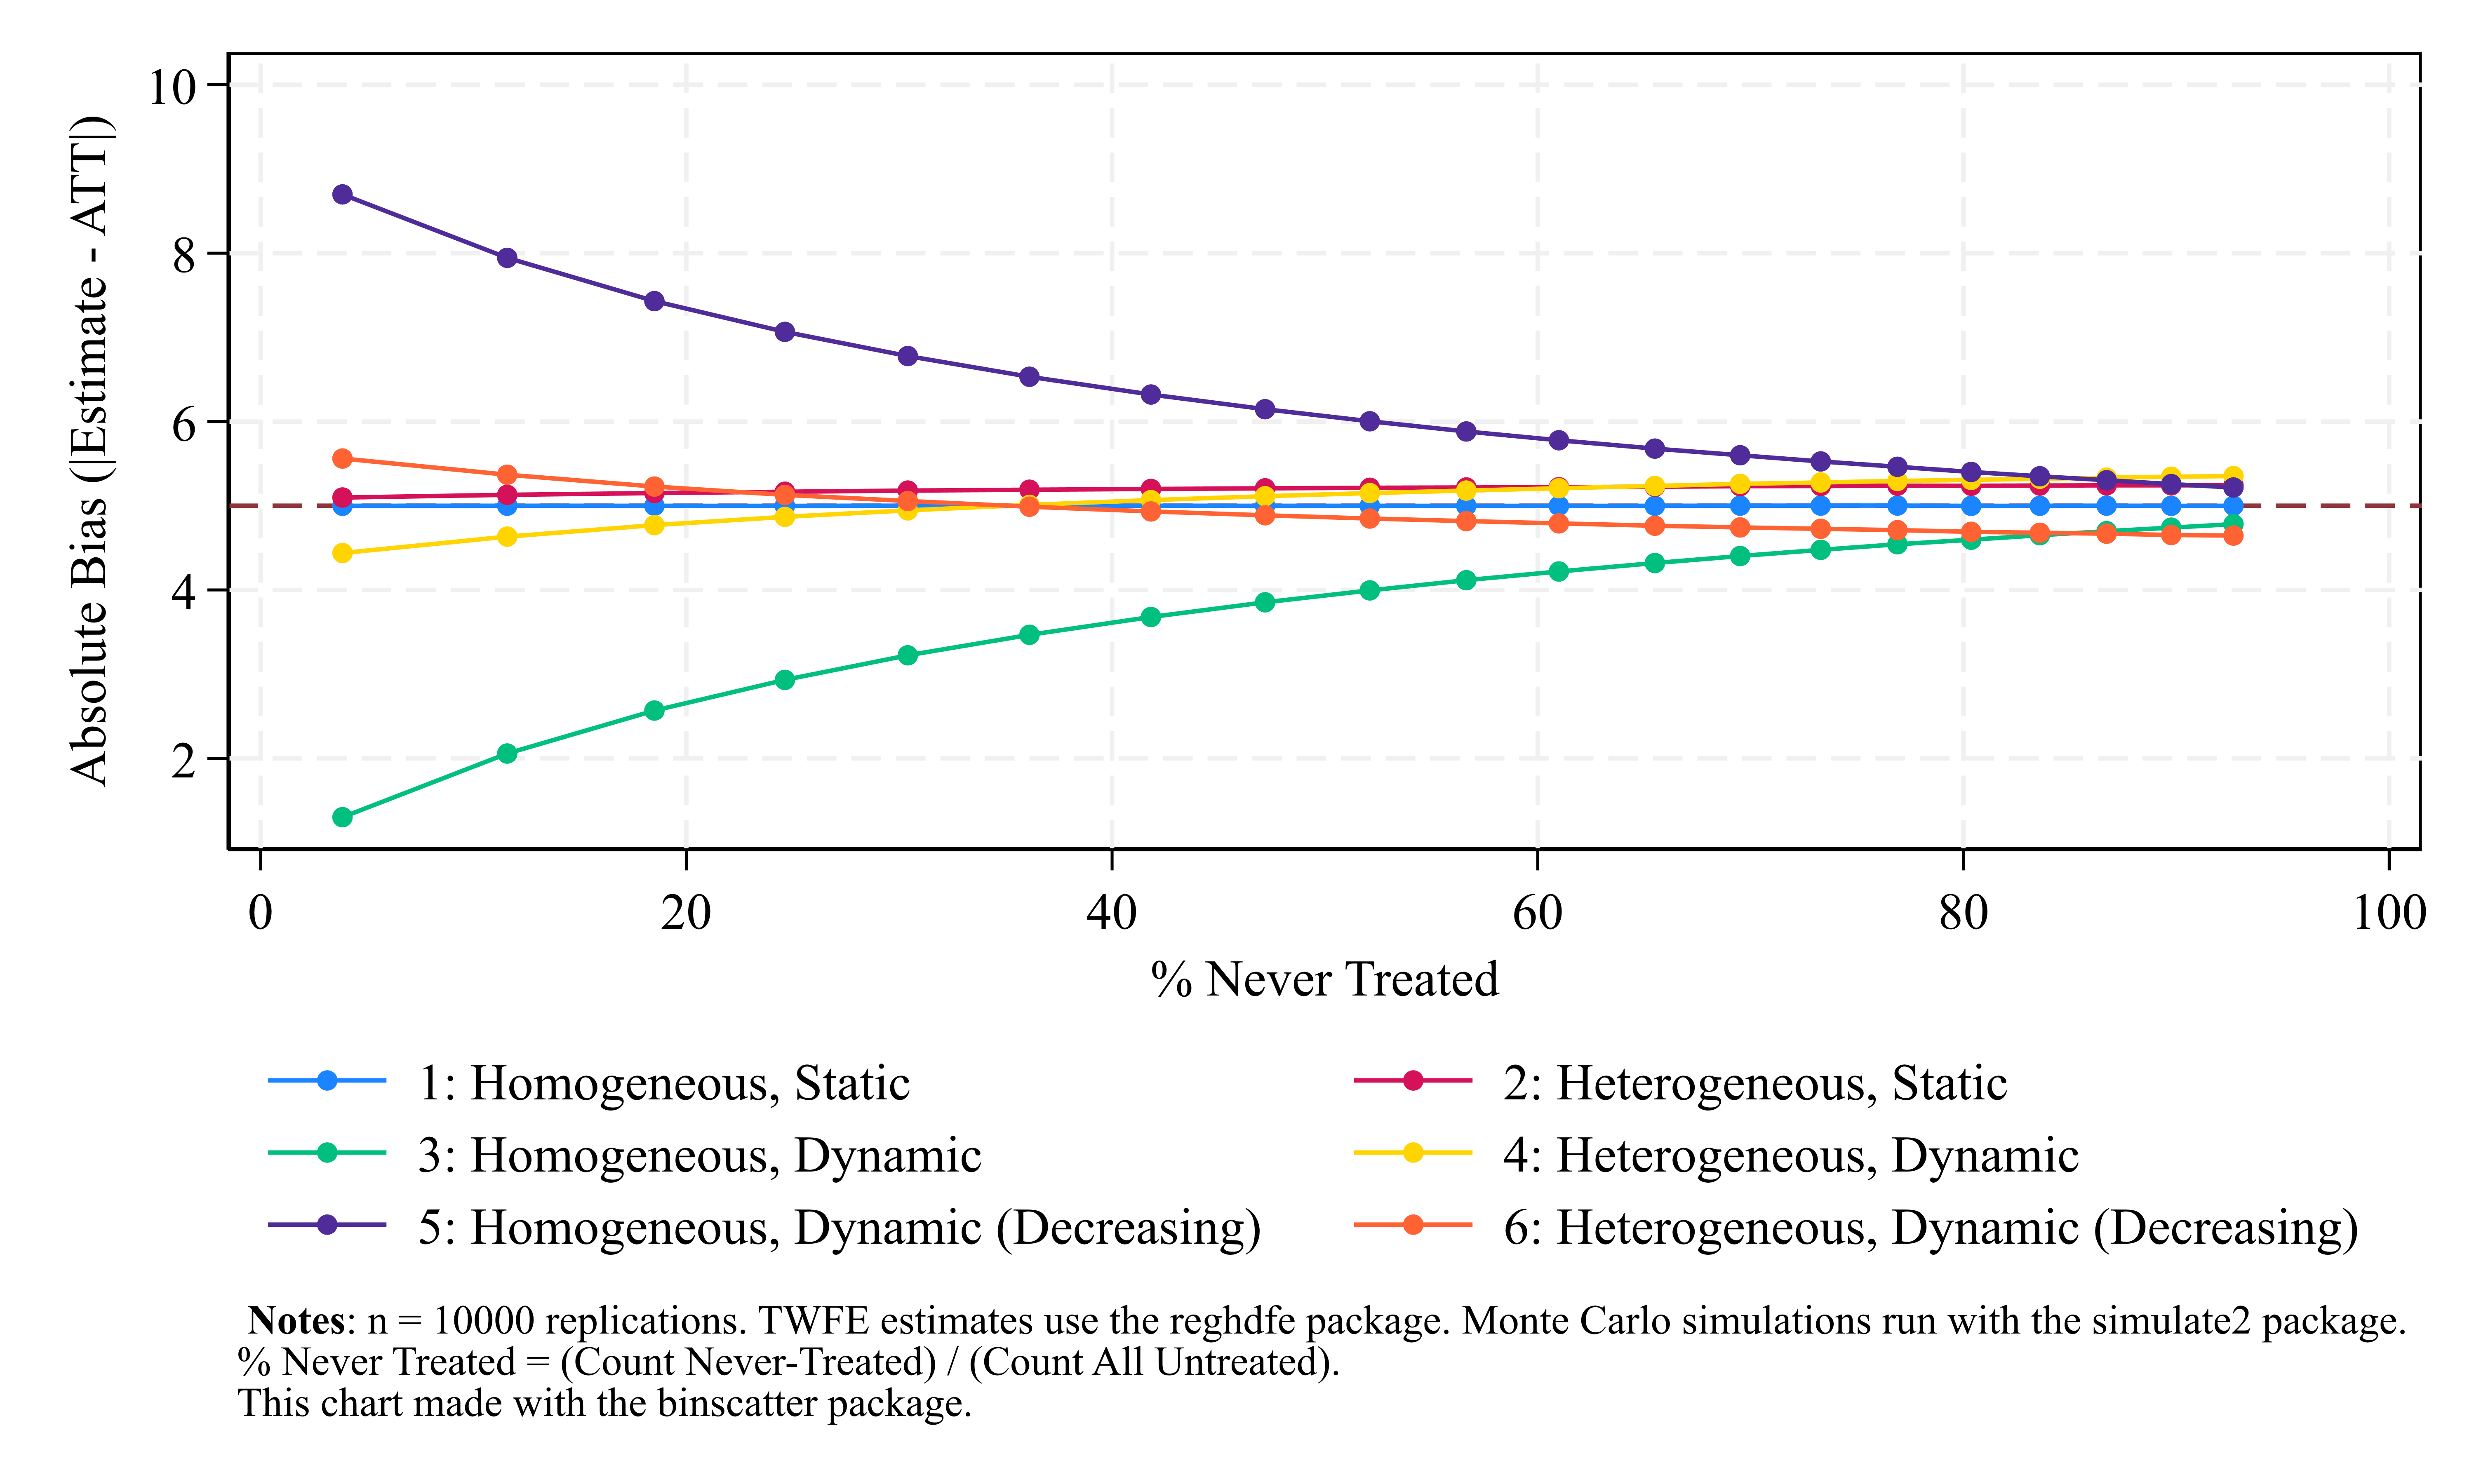
\includegraphics[width=6in]{Figures/TWFE Bias by Percent Never Treated.png}
    \label{fig:pc-nevertreat}
\end{figure}
\subsubsection{DiD Estimator Bias for Unbalanced Panels}
To investigate the effects of unbalanced data on DiD estimators, we randomly generate 10,000 datasets with varying degrees of balance and run TWFE models on them.\footnote{We create entry and exit by choosing a “cutoff” point uniformly distributed between 0 and 0.5, then generating observation-specific flags for another uniform variable being below the cutoff. The unit’s entry date is the first time that the flag is on, and the exit date is the last time that the flag is on. We then implement filters to prevent instances where the entry and exit dates are the same for a unit. The cutoff varies among datasets.}  Figure \ref{fig:pc-balance} below reports the average bias from each of the 6 treatment effects by \% Balanced, where a value of 100 indicates a balanced panel, and 50 indicates that half of the data is missing compared to a balanced panel.\footnote{Our method of simulating the data means that unbalanced panels have fewer observations than more balanced ones. We compensate by increasing the balanced size to 50,000 observations (instead of 20,000) and running 10,000 simulations (instead of 1,000). \hyperref[sec:appendixb]{Appendix B} reports scatterplots of each simulated result to demonstrate the increasing spread of bias due to smaller samples.}
\begin{figure}[H]
    \centering
    \caption{TWFE Bias by Percent Balanced Data}
    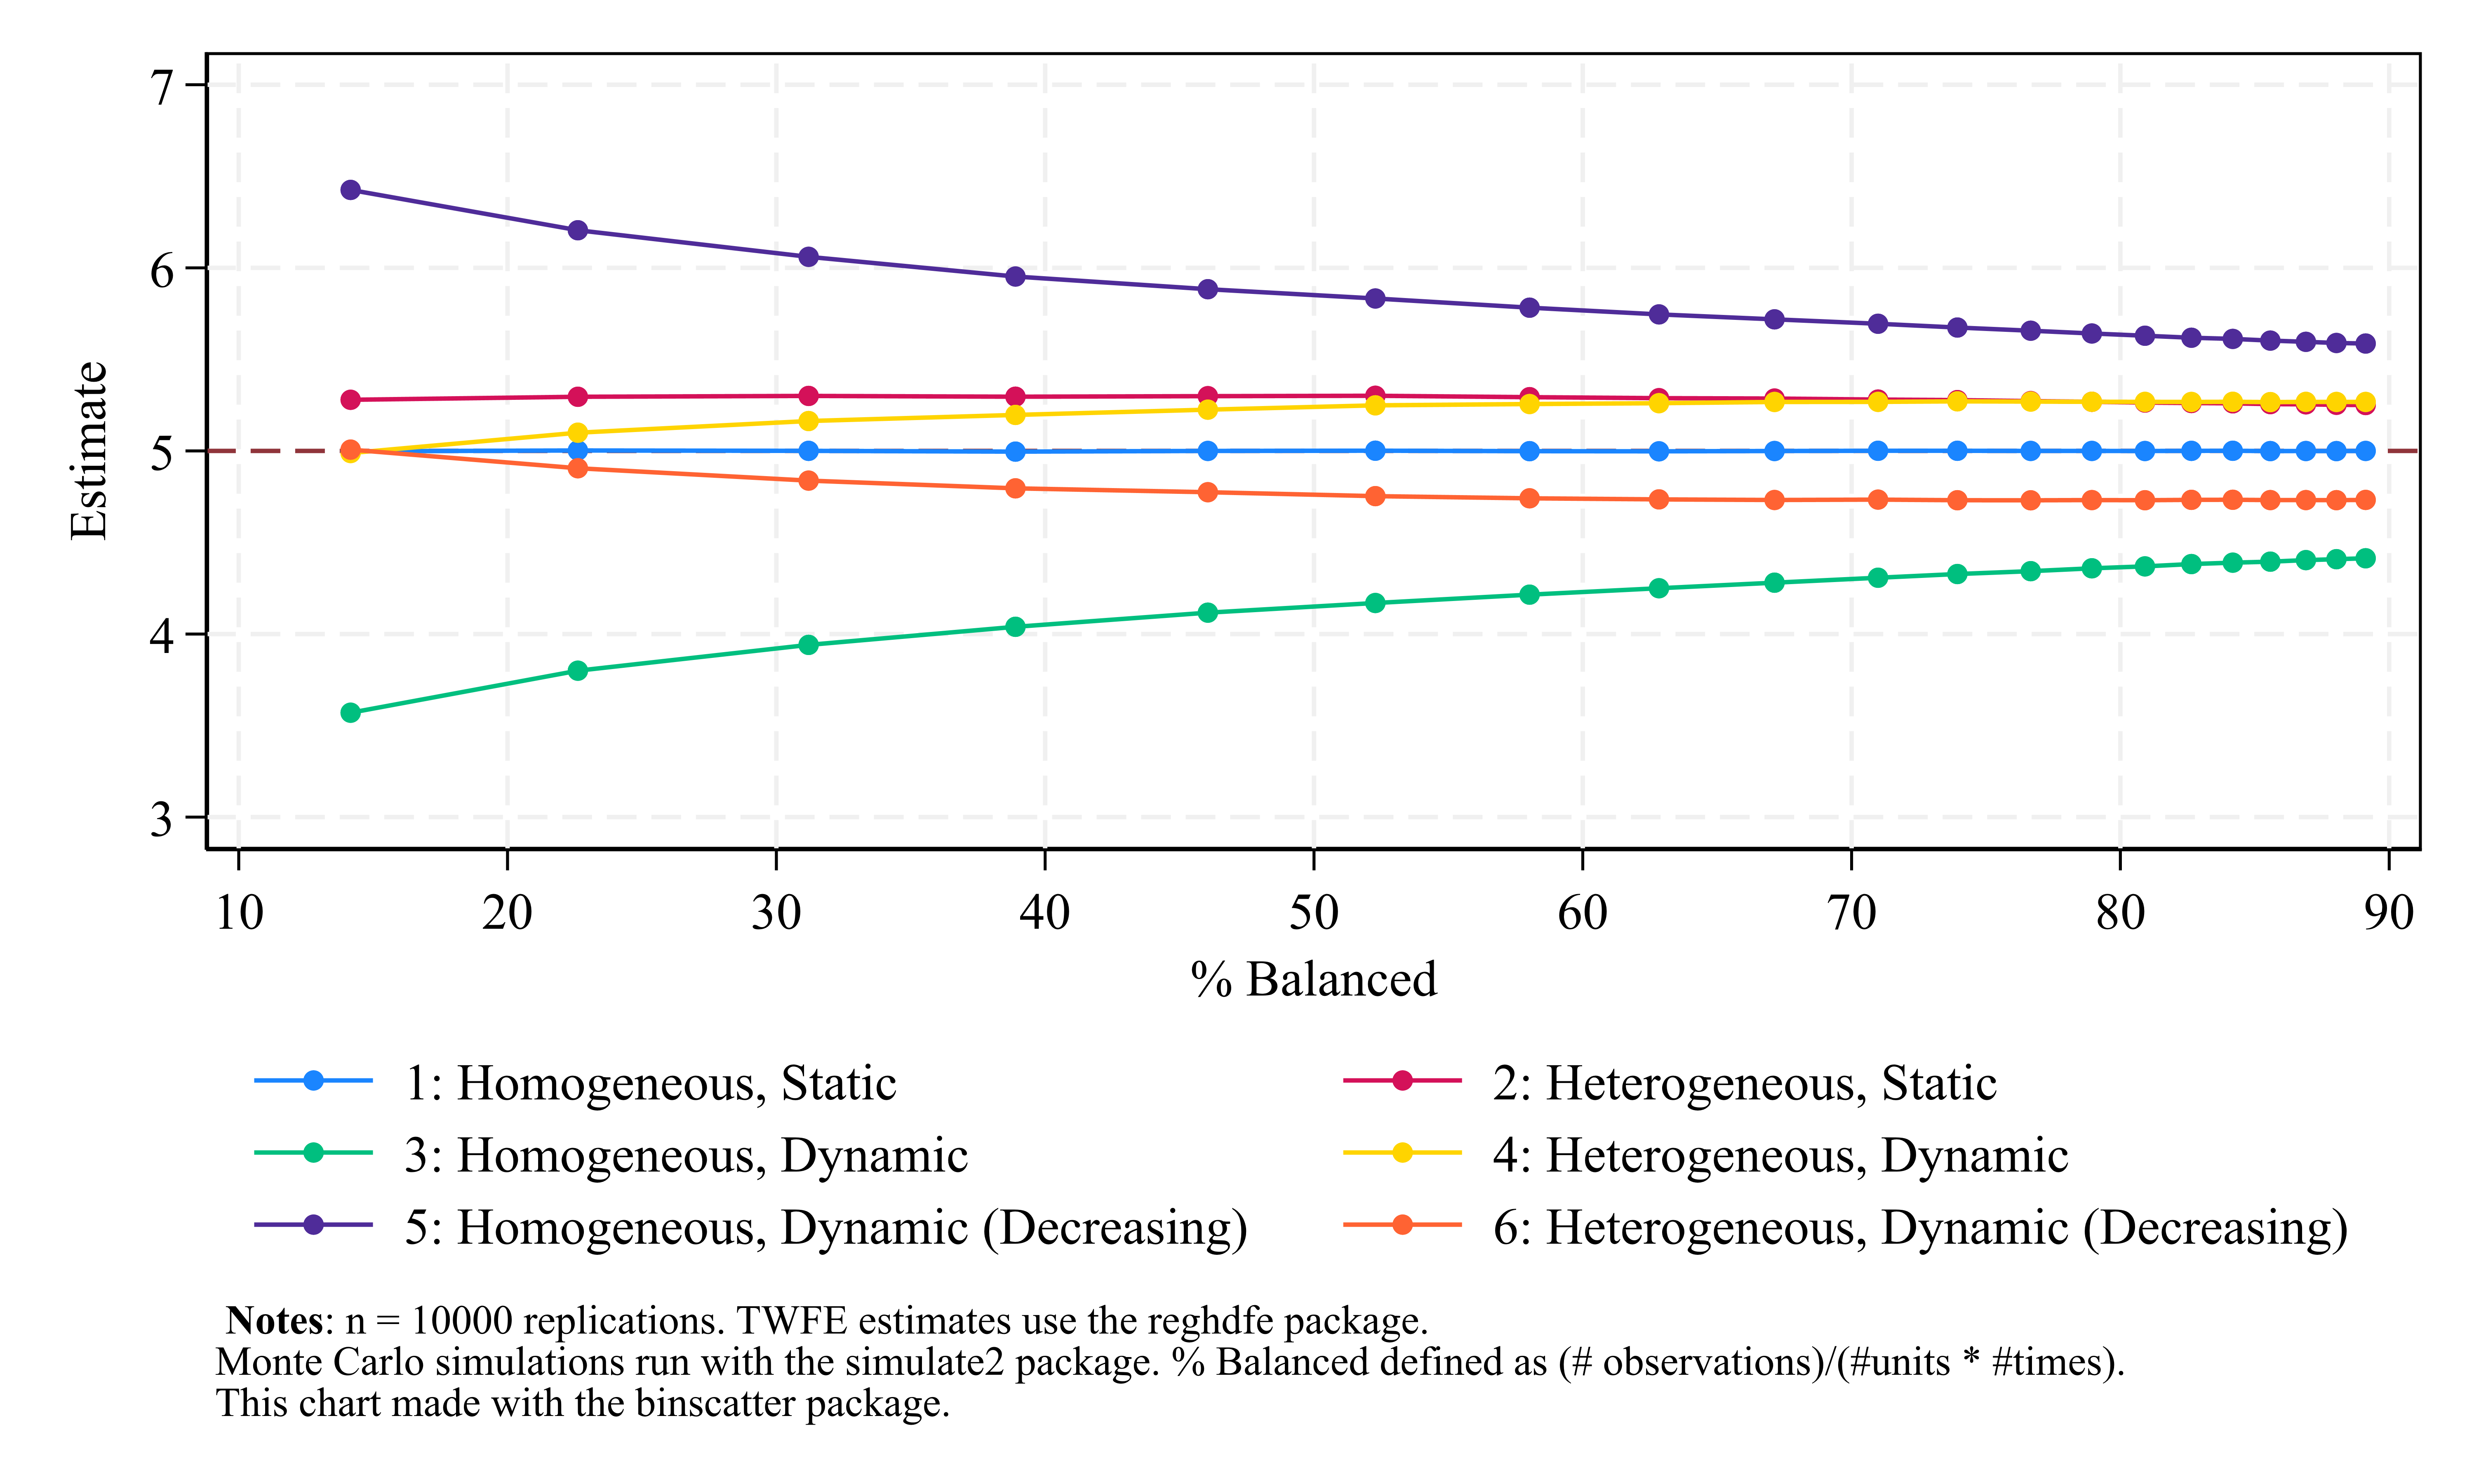
\includegraphics[width=6in]{Figures/TWFE Bias by Percent Balanced Crop.png}
    \label{fig:pc-balance}
\end{figure}
\noindent
Our analysis shows that TWFE bias depends on how unbalanced the panel is when treatment effects are dynamic, even if the exit and entry is not a function of treatment status. Bias is substantially lessened for balanced panels when treatment effects are homogeneous and dynamic, but it increases slightly when treatment effects are heterogenous and dynamic.

Now, we compare the TWFE bias for unbalanced panels to the new estimators. First, we observe biased estimators for highly unbalanced panels in all estimators \uline{except the Sun and Abraham model}. This is particularly interesting given our reported equivalence between that estimator and the Callaway and Sant’Anna model in a balanced setting. Bias only occurs for the new estimators when the treatment effect is dynamic (datasets 3 through 6), though bias is very small when those dynamic effects are heterogeneous (datasets 4 and 6). We see that all the new estimators converge to the correct effect as the data becomes more balanced, while that is not true for the TWFE estimators. Finally, note that the direction of the bias is the same for all estimators within a dataset: when treatment effects increase over time (dataset 3), bias is negative, and vice versa when treatment effects decrease over time (dataset 5).\footnote{While exit and entry in our simulated data is not a function of treatment status, it is correlated indirectly. To investigate, we combined 100 randomly generated datasets using the same method as in our analysis, and stacked the data. Examining \hyperref[fig:dist-treat]{the distribution of the data over time}, we see that the earliest and latest periods of treatment status are most likely to be removed from the data, explaining the direction of bias. See \hyperref[sec:appendixb]{Appendix B}.}
\begin{figure}[H]
    \centering
    \caption{Statistical Comparison of DiD Methods with True Average Effect by Percent Balanced}
    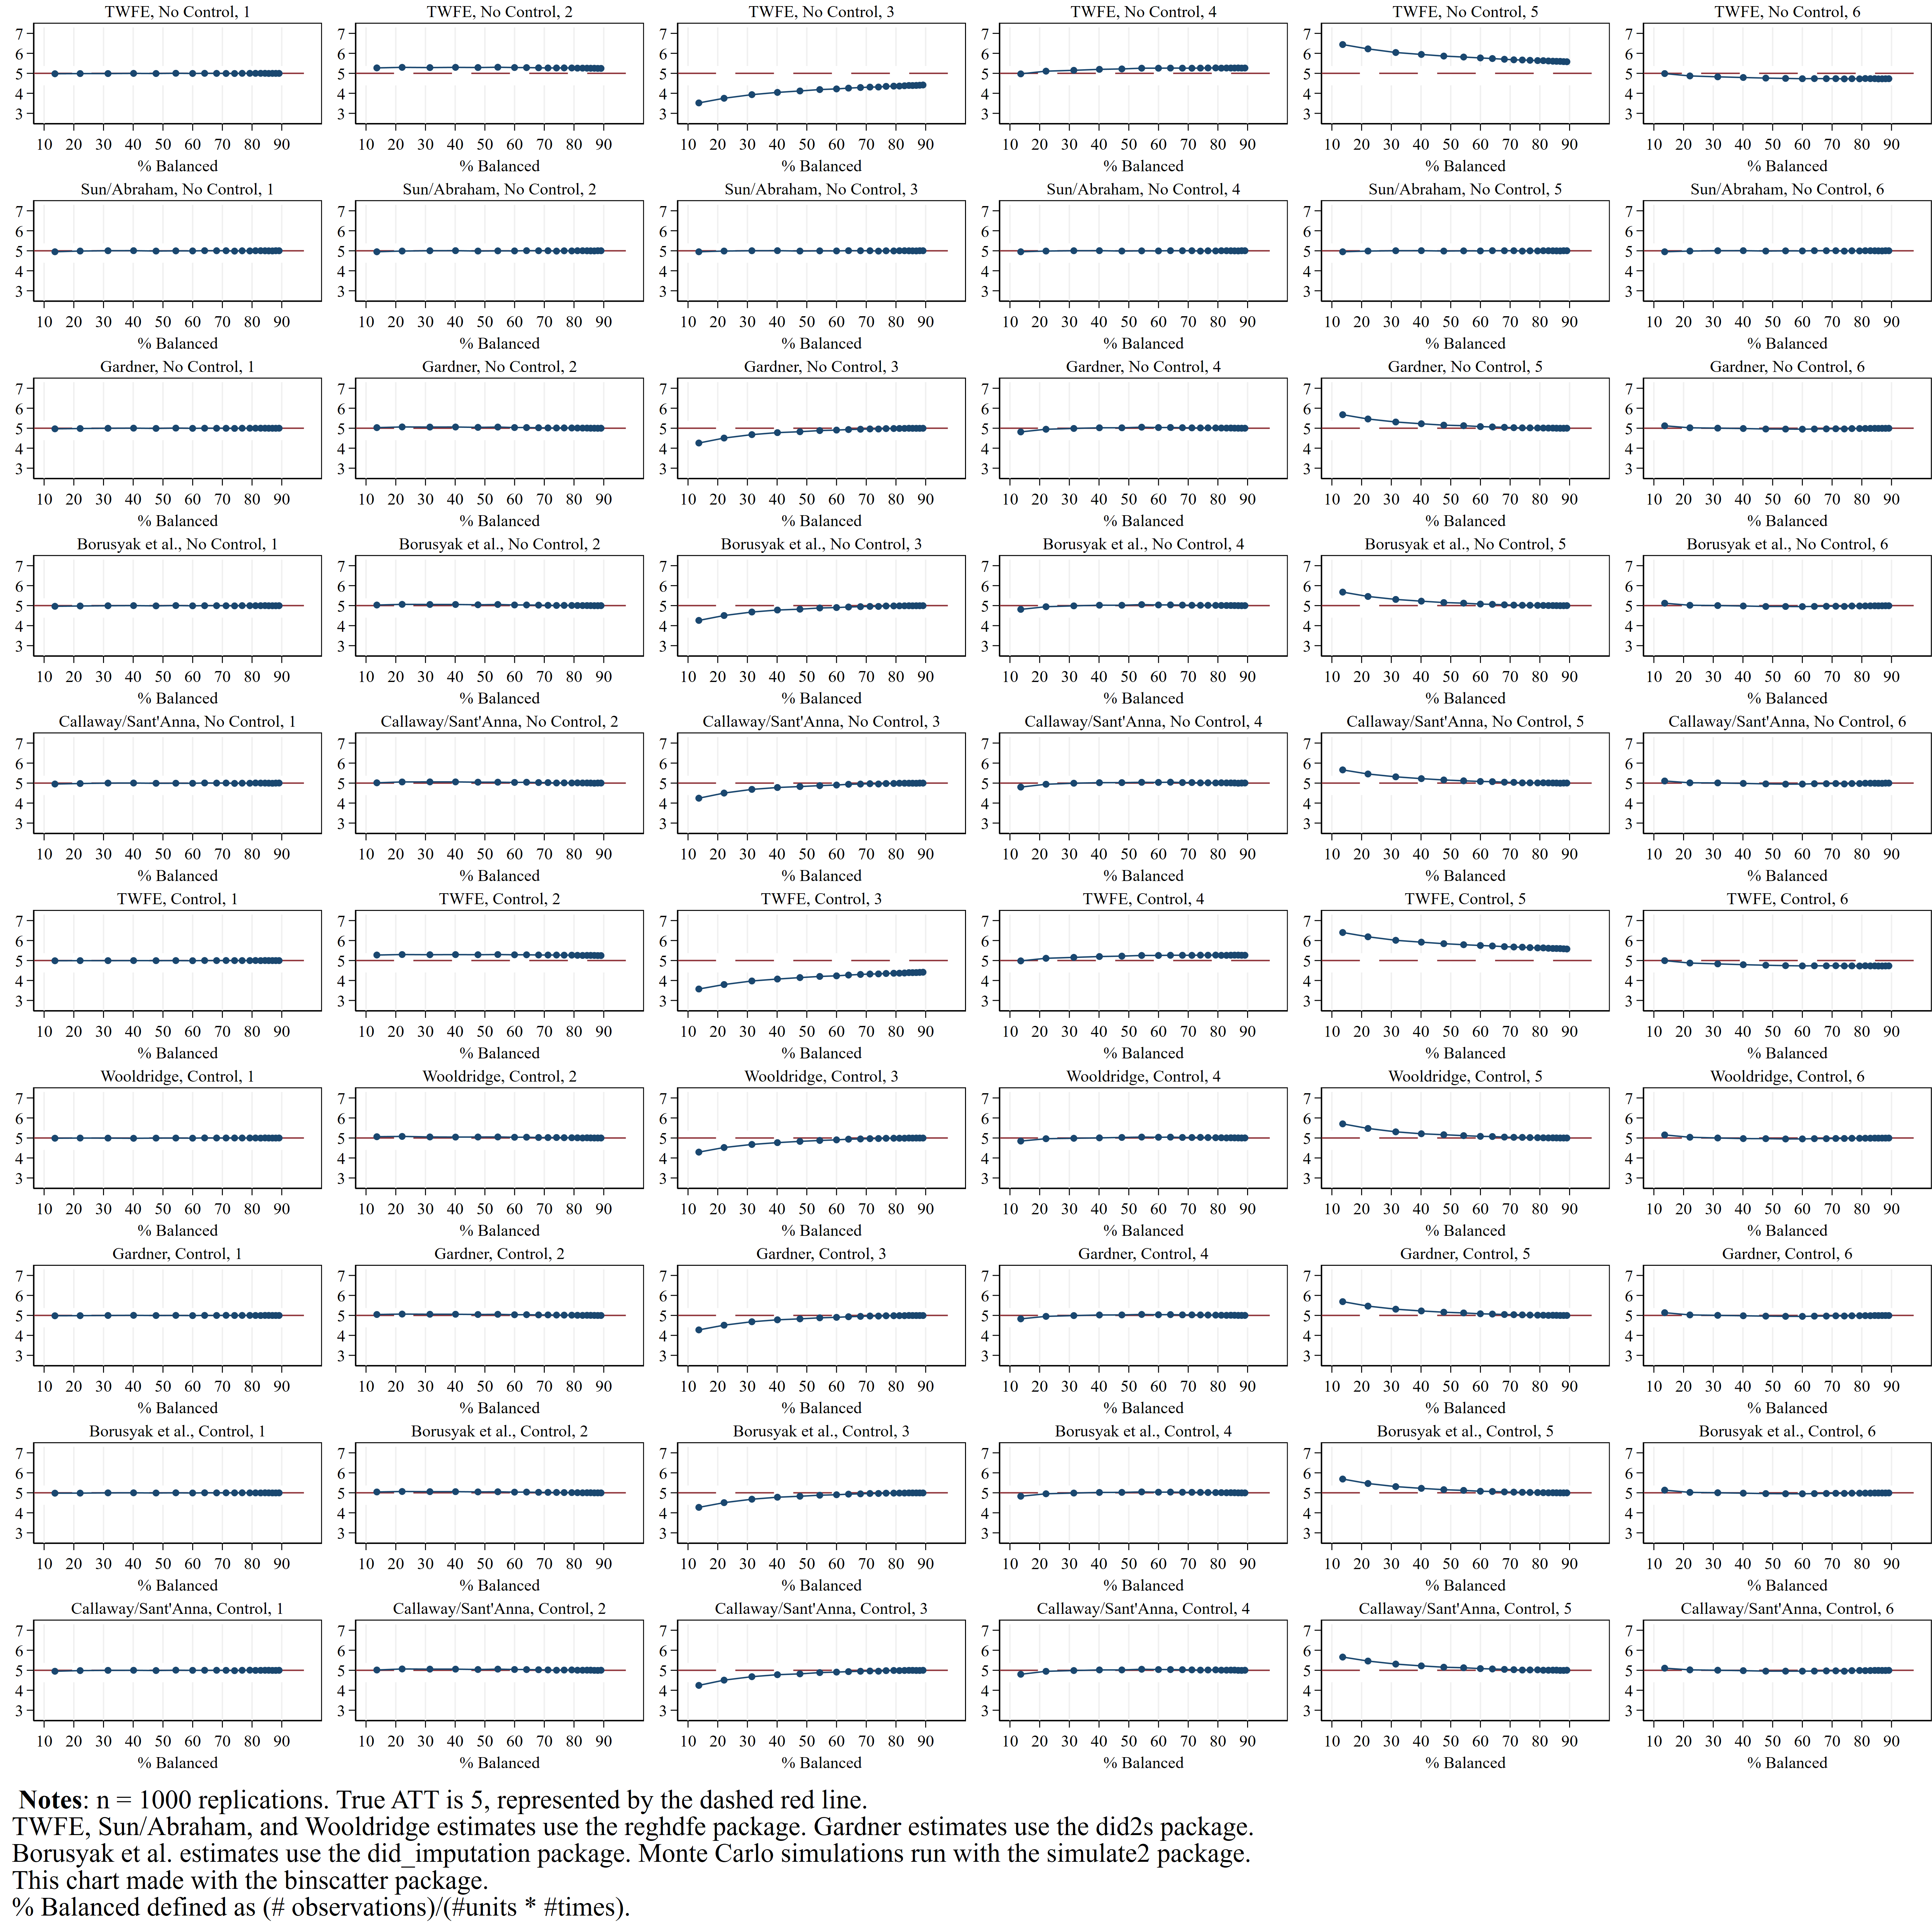
\includegraphics[width=6in]{Figures/Binscatters by Percent Balanced Common Scale.png}
    \label{fig:estimators-balanced}
\end{figure}
\section{Conclusion} \label{sec:conclusion}
\singlespace
Difference-in-differences analysis is one of the most important techniques for policy evaluation in the social sciences, and will continue to be used frequently in antitrust work. The recent literature has shown that traditional DiD techniques are subject to mismeasurement under a variety of realistic situations. But this literature has also provided a suite of new tools that can examine policy effects with more detail and clarity than ever before. We reviewed the new estimators and discussed their strengths and weaknesses as it pertains to common antitrust analysis. Our Monte Carlo analysis confirms findings from the literature, and it exposes unbalanced data as a source of bias that even the new estimators can mismeasure. Our discussions and list of recommended sensitivities will hopefully provide antitrust practitioners and other applied economists with the rigor needed for DiD work going forward.

\newpage
\doublespace
\printbibliography

\newpage
\section*{Appendix A. Recommended Sensitivities} \label{sec:appendixa}
\addcontentsline{toc}{section}{Appendix A. Recommended Sensitivities}
Here we provide a list of recommended sensitivities when performing staggered DiD analysis. Practitioners can use this as a reference checklist to ensure the robustness of their results. Substantial deviations in any sensitivities may call for a closer look at your model and assumptions. Similarly, this checklist could be used by experts responding to a DiD analysis as a method for evaluating its robustness. Conclusions will always depend on circumstances of the case, including data availability. Passing or failing any of these tests does not necessarily validate or invalidate a result. Finally, this list is not comprehensive with respect to general model specification sensitivities, only to characterize the robustness of the DiD itself; additional checks on functional form, appropriate controls, and others still apply.
\begin{enumerate}
    \item Sensitivities on appropriate control group:
    \begin{enumerate}
        \item Use never-treated only as the control group
        \item Use not-yet-treated only as the control group
        \item Use both never-treated and not-yet-treated
        \item Perform tests to assess whether the not-yet-treated and never-treated groups are systematically different. For example, you might run placebo tests where the not-yet-treated group is a pseudo-treatment group, and never-treated is the pseudo-control. This can also reveal anticipation effects if the not-yet-treated units have different behavior than the never-treated.
    \end{enumerate}
    \item Sensitivities on heterogeneous treatment effects:
    \begin{enumerate}
        \item Estimate cohort-time interacted effects and perform Wald tests among DiD coefficients. Accomplish this with some form of the Wooldridge ETWFE estimator (or Sun/Abraham with no coefficients), depending on computation limits and context-specific knowledge of treatment effect heterogeneity. If the Wald tests show treatment effects are not equal between cohorts, consider incorporating cohort-specific treatment effects in the model.
        \item Aggregate the cohort-time specific treatment effects by observed probabilities  as well as other relevant metrics like revenue or volume.\footnote{\citet{sunabr2021a}, p. 186 (Section 4.1).}  Compare these results to the single-coefficient TWFE or standard DiD model.
        \begin{enumerate}
            \item Importantly, assess the economic significance of any difference between a TWFE model and the new estimators. In our experience, in big datasets, the statistical significance of such a difference may not solely determine whether TWFE model is inappropriate.
        \end{enumerate}
        \item Run an imputation-style estimator (Gardner or Borusyak et al.), especially if you prefer to estimate a single DiD coefficient.\footnote{\citet{gardner2022a}, Section 3. \citet{borusyak2024revisiting}, p. 16 (Theorem 2).}  These estimators can be very quick (and thus attractive for large data), but they have limitations with unbalanced panels as described above. If including covariates in the model, be mindful of the implicit assumption that covariates do not affect treatment status and vice versa.\footnote{See \citet{gardner2022a}, note 9. Be prepared to support this assumption with additional analysis.}  These models make explicit but-for predictions for the treatment group that can be aggregated many different ways. This can be useful for assessing systematic differences present in the data.
        \item Run a Sun and Abraham-style auxiliary regression (Their equation 13 following Proposition 1) to estimate TWFE treatment weights. Can also use the method from \citet{borusyak2024revisiting} Proof of Proposition 2. Assess relationships between these weights and observables such as time. This is especially useful when binning the data, as demonstrated in \citet{borusyak2024revisiting} Section 5.2.1.
         \begin{enumerate}
            \item If using a TWFE-style model, examine the weights over many subsets of the data. For example, see if certain subsets get systematically negative weight, and understand how that might bias your results. For examples of visualizations of negative weights, see \citet{jakiela2021a}, Figures 2 through 4.
        \end{enumerate}
        \item Consider whether the treatment effect may vary by other observables, and measure them separately if needed. For example, are certain products likely to see higher price increases from a conspiracy? Or, in a class action context, it could be that some groups of customers were not affected by the alleged conduct. While measuring many separate treatment effects can be useful, doing so to intentionally lower the precision of someone’s model is bad practice. Further, using iterated regressions to find a subset of units with no treatment effect is subject to model selection bias.
    \end{enumerate}
    \item Sensitivities on parallel trends:
    \begin{enumerate}
        \item \label{butfor-item} Use your preferred model to predict the but-for outcome for treated observations. Then compare but-for outcomes to observed outcomes before the treatment starts, for example by plotting these lines for each treated unit. This method tests whether your control group provides a good approximation to your treatment group before the treatment.
        \item Run a Sun and Abraham- or Wooldridge-style cohort-interacted event study with the full set of indicators relative-time indicators (including negative exposure times), then assess the pre-treatment coefficients.
        \item Run a \citet{borusyak2024revisiting}-style placebo test on untreated observations.\footnote{\citet{borusyak2024revisiting}, p. 21 (Test 1). Note their discussion of alternative placebo tests and their associated drawbacks in pp. 21-22.
        \\\\
        Keep in mind the visual interpretation guidelines from \citet{roth2024a} for new estimators. In particular, the Borusyak et al. imputation estimator pre-trend coefficients should be considered separately from post-trend coefficients. \citet{roth2024a}, Section 3.3.}
        \item Assess maximal parallel trend violations and use it to size the possible impact to your treatment effect.\footnote{\citet{rambachan2023more}, Section 6.2, and Figures 5 and 7 in particular.}
        \item Assess whether postestimation parallel trends tests are likely to be underpowered in the available data.
        \item Estimate a model with product-specific time trends in the style of \citet{wooldridge2021two}, Equation 7.14 (which substitutes time fixed effects for unit-specific time trends).\footnote{Stata’s popular third-party package \texttt{reghdfe} allows for faster estimation of these types of models if you do not care about the coefficients of the unit-specific time trends (also called fixed slopes estimation). See also \citet{ruttenauer2023fixed} and their package \texttt{xtfeis}.}  This relaxes the parallel trends assumption to an assumption that treated units would have continued their pre-treatment trend but for the treatment effect.\footnote{\citet{ruttenauer2023fixed} is an excellent resource for panel models with unit-specific trends. They discuss the benefits and drawbacks of adding these time trends to your model. They specify Hausman-style tests of unit-specific trends vs fixed or random effects models (interpretable as a parallel trends test). Finally, they provide a wealth of citations both for and against this type of model.}  This can also be used as evidence in favor of (or against) common trends. With enough data, you can add polynomial terms to the model to allow for more flexible differences in pre-trends.\footnote{For example, your regression could have product fixed effects (FE), then product FE interacted with (continuous) time, product FE interacted with time squared, and so on. These models do not include time FE. But keep in mind that this specification will remove products with few observations, which can be especially problematic with unbalanced panels. \citet{ruttenauer2023fixed}, p. 74.}  Visually compare the fit from this model to the method described in sensitivity \ref{butfor-item}.
    \end{enumerate}
    \item Sensitivities on selection bias:
    \begin{enumerate}
        \item Test for correlation between treatment status and observables with an auxiliary regression using treatment status as your outcome variable.
        \item Perform typical panel attrition tests.\footnote{\citet{wooldridge2010a}, Chapter 17.7.3.}  Include an indicator for “drops out of data in next period” in your model and assess its coefficient. Are certain groups in the data more likely to exit than others?
        \item To the extent that exit bias may exist, try to evaluate the expected direction of the bias. For example, if customers drop out because their price becomes too high, and you’re modelling prices, consider whether your treatment effect is underestimated.
    \end{enumerate}
    \item Sensitivities for entry and exit in both control and treatment groups:
    \begin{enumerate}
        \item Estimate your model by removing all agents that are partially in the data before and after the policy date.
        \item Remove agents that are only in the before period\footnote{Depending on the policy of interest, it can be possible to identify a product or customer that drops out of the data \textit{before} they start their treatment. For example, you may have outside information that identifies treatment status.} or only in the after period (always-treated). Test whether they significantly change the estimate of the policy effect.
        \item If there are treatment agents that enter into the data after the policy is implemented (always-treated), perform analysis to determine if the new treatment entrants are different from the other treated agents. If they are different, try to adjust the model such that you can estimate the policy effect. For example, if a new store opens in a county after the start of a conspiracy, try to measure the effect of the conspiracy using stores in the same county or the same owner in a nearby county.
        \item If going forward with a TWFE model, use the estimated weight techniques from above to assess the always-treated group in detail. Beware that it can be highly subject to negative weighting issues.
        \item Compare a Sun and Abraham-style estimators to any other new estimators used, especially when the data is highly unbalanced. A large difference between the two may indicate bias stemming from treatment status correlated with entry and exit.
    \end{enumerate}
\end{enumerate}
\newpage
\section*{Appendix B. Additional Monte Carlo Results} \label{sec:appendixb}
\addcontentsline{toc}{section}{Appendix B. Additional Monte Carlo Results}

\begin{figure}[H]
    \centering
    \caption{Distributions of Monte Carlo Estimates in Table \ref{tab:estimators-never}}
    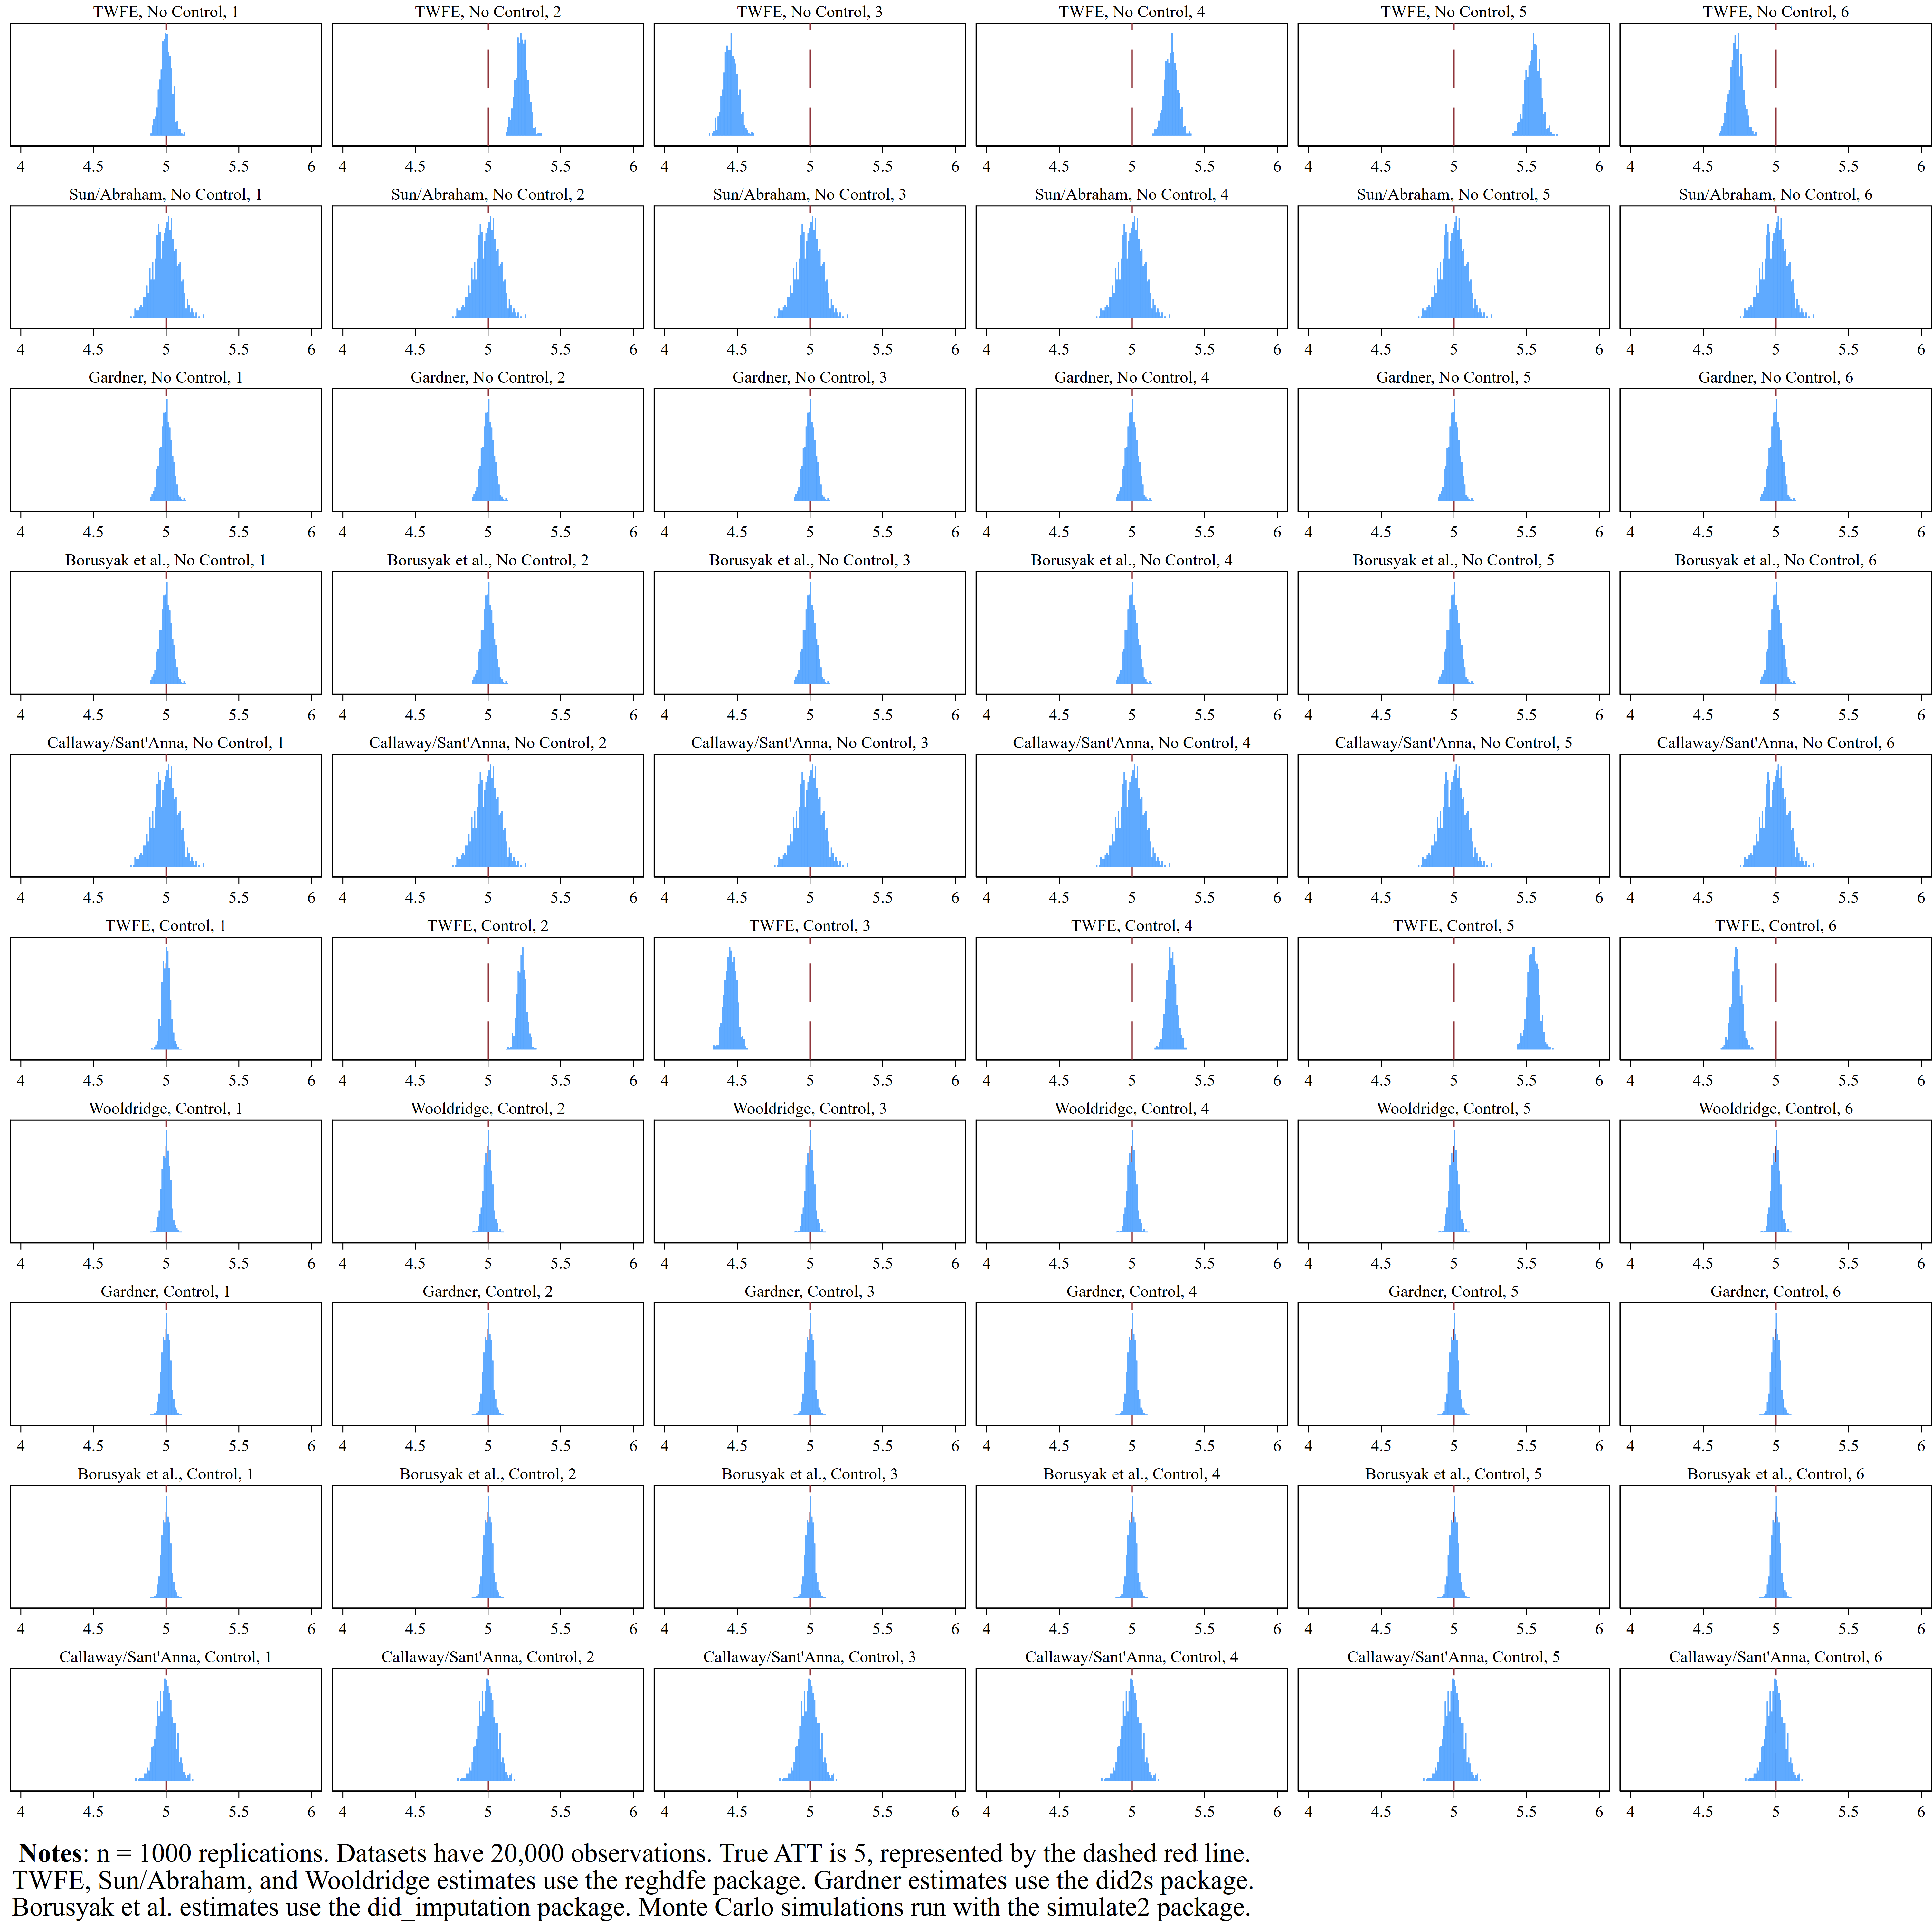
\includegraphics[width=6in]{Figures/Histograms of Monte Carlo Estimates 1.png}
    \label{fig:hist1}
\end{figure}

\begin{figure}[H]
    \centering
    \caption{Distributions of Monte Carlo Estimates in Table \ref{tab:estimators-notyet}}
    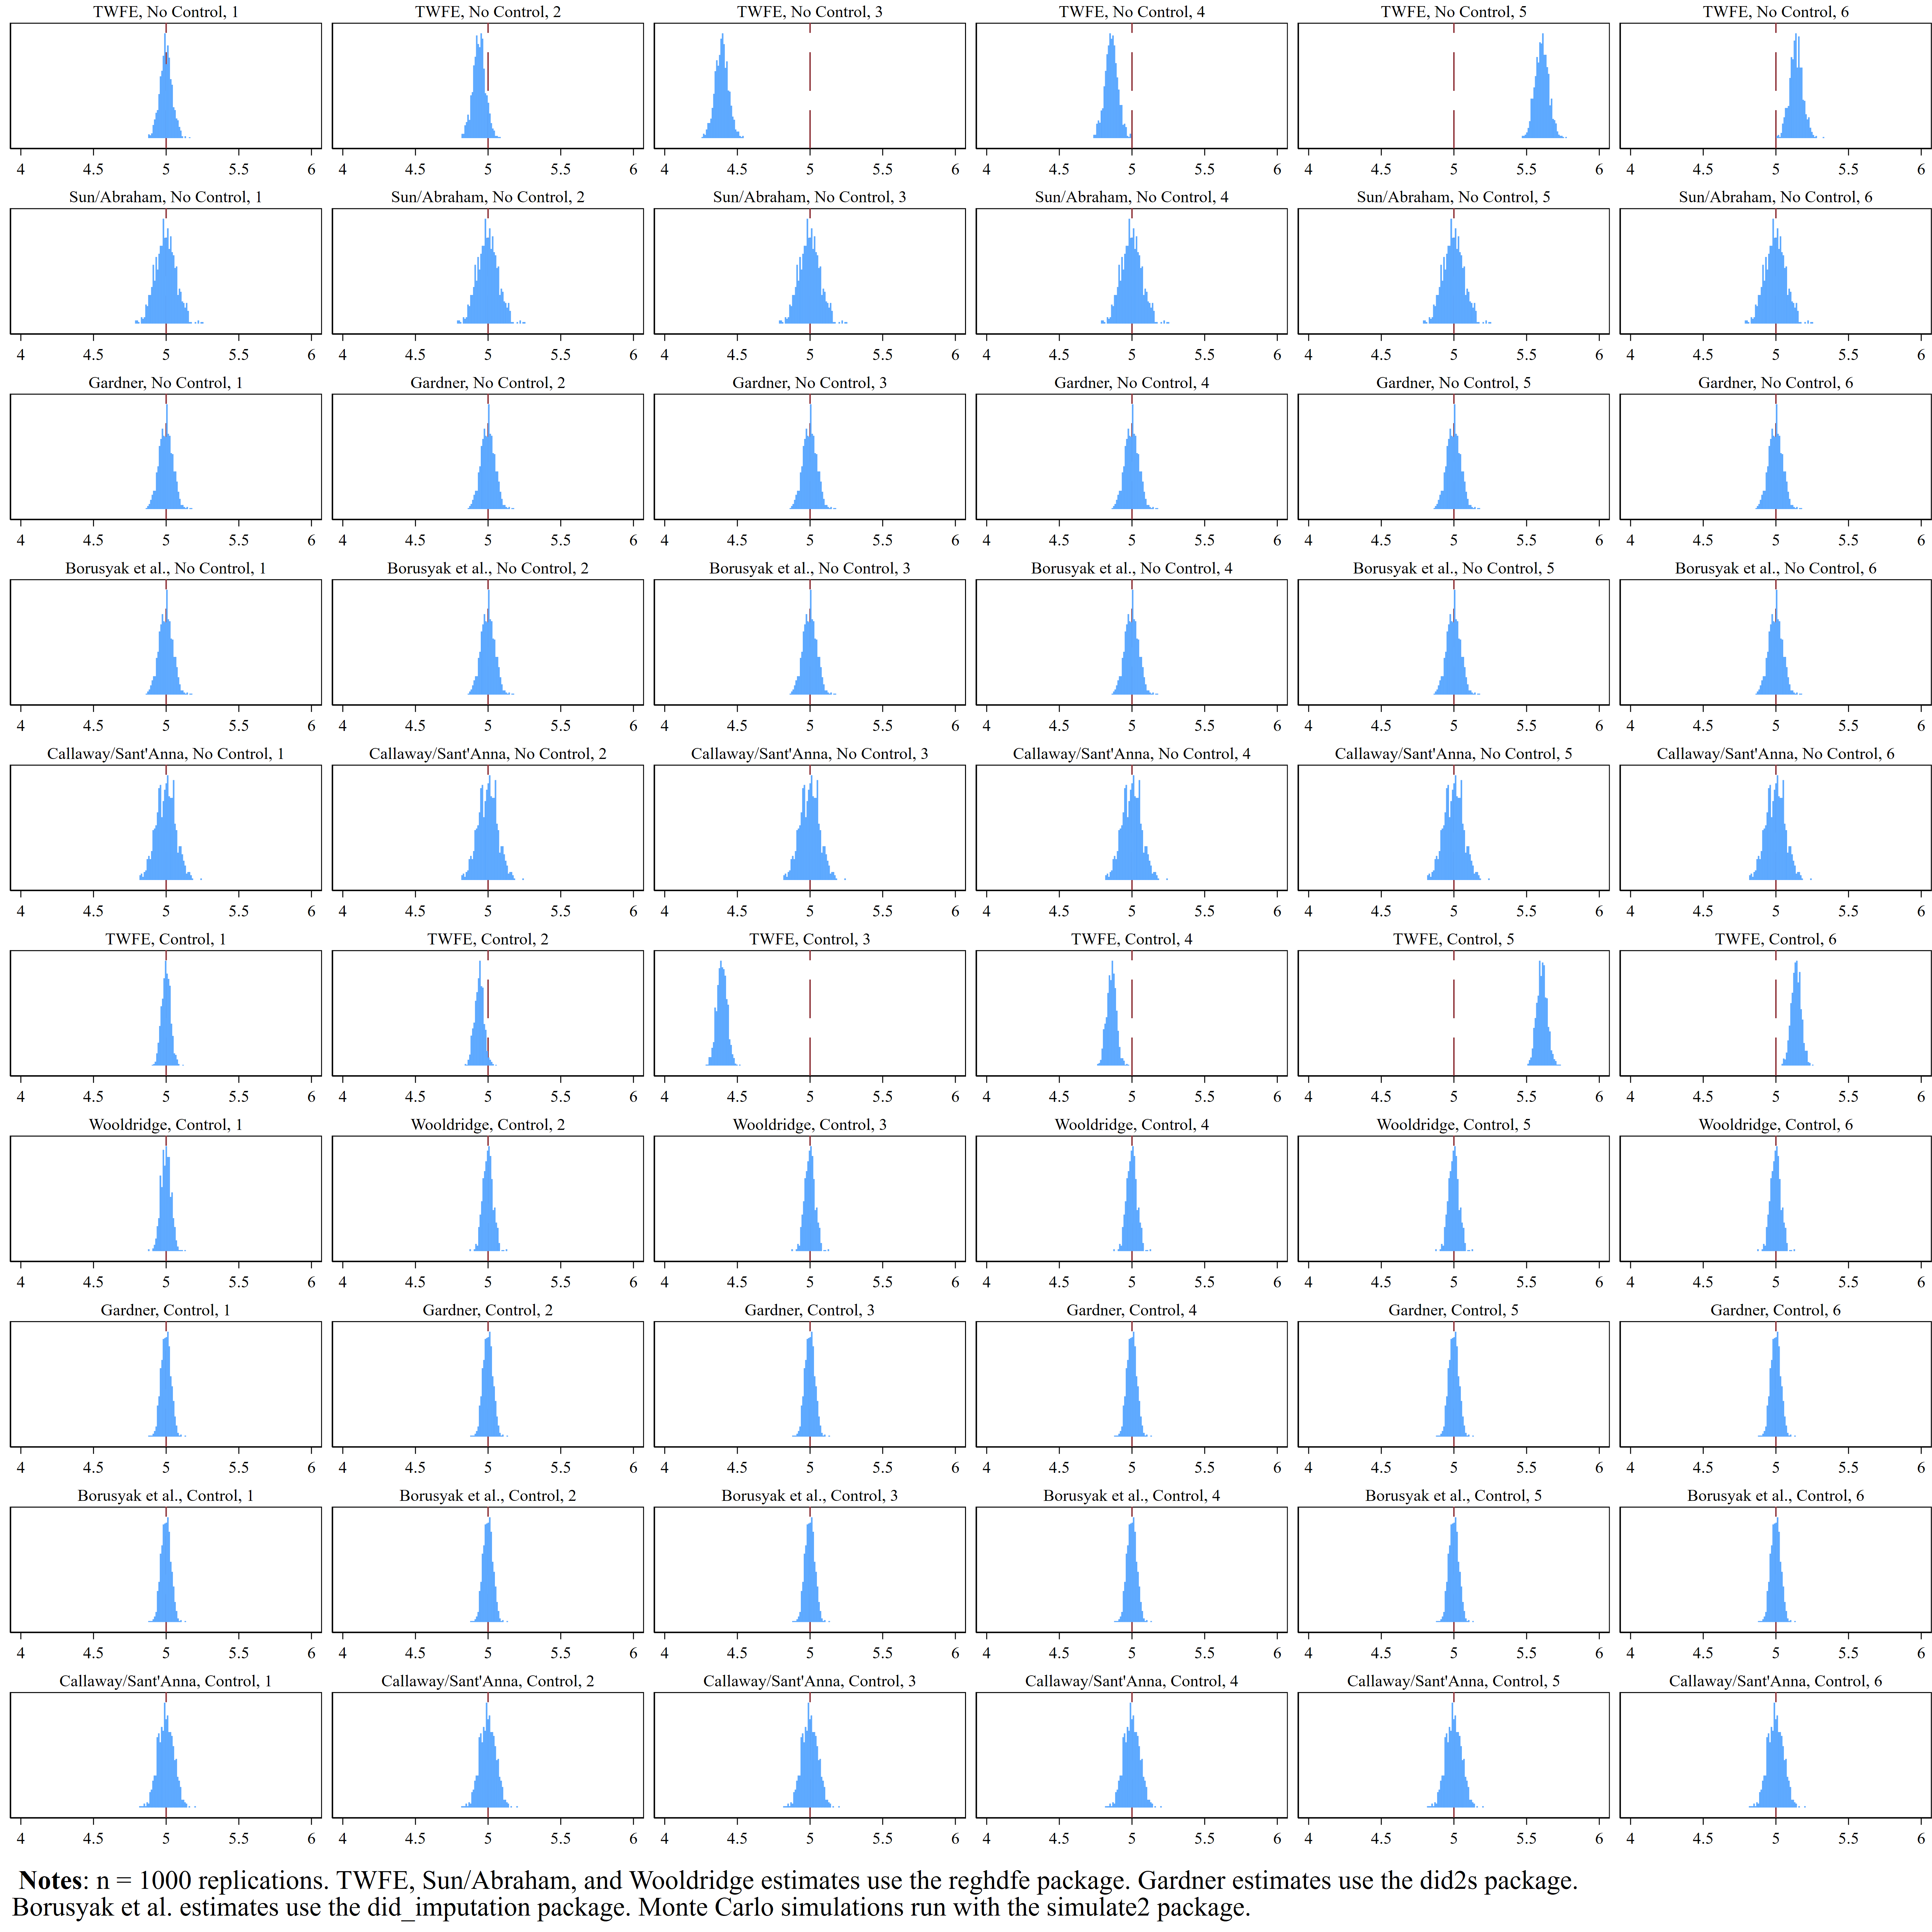
\includegraphics[width=6in]{Figures/Histograms of Monte Carlo Estimates 2.png}
    \label{fig:hist2}
\end{figure}

\begin{figure}
    \centering
    \caption{TWFE Bias by Percent Never-Treated in the Data (Scatter Plot)}
    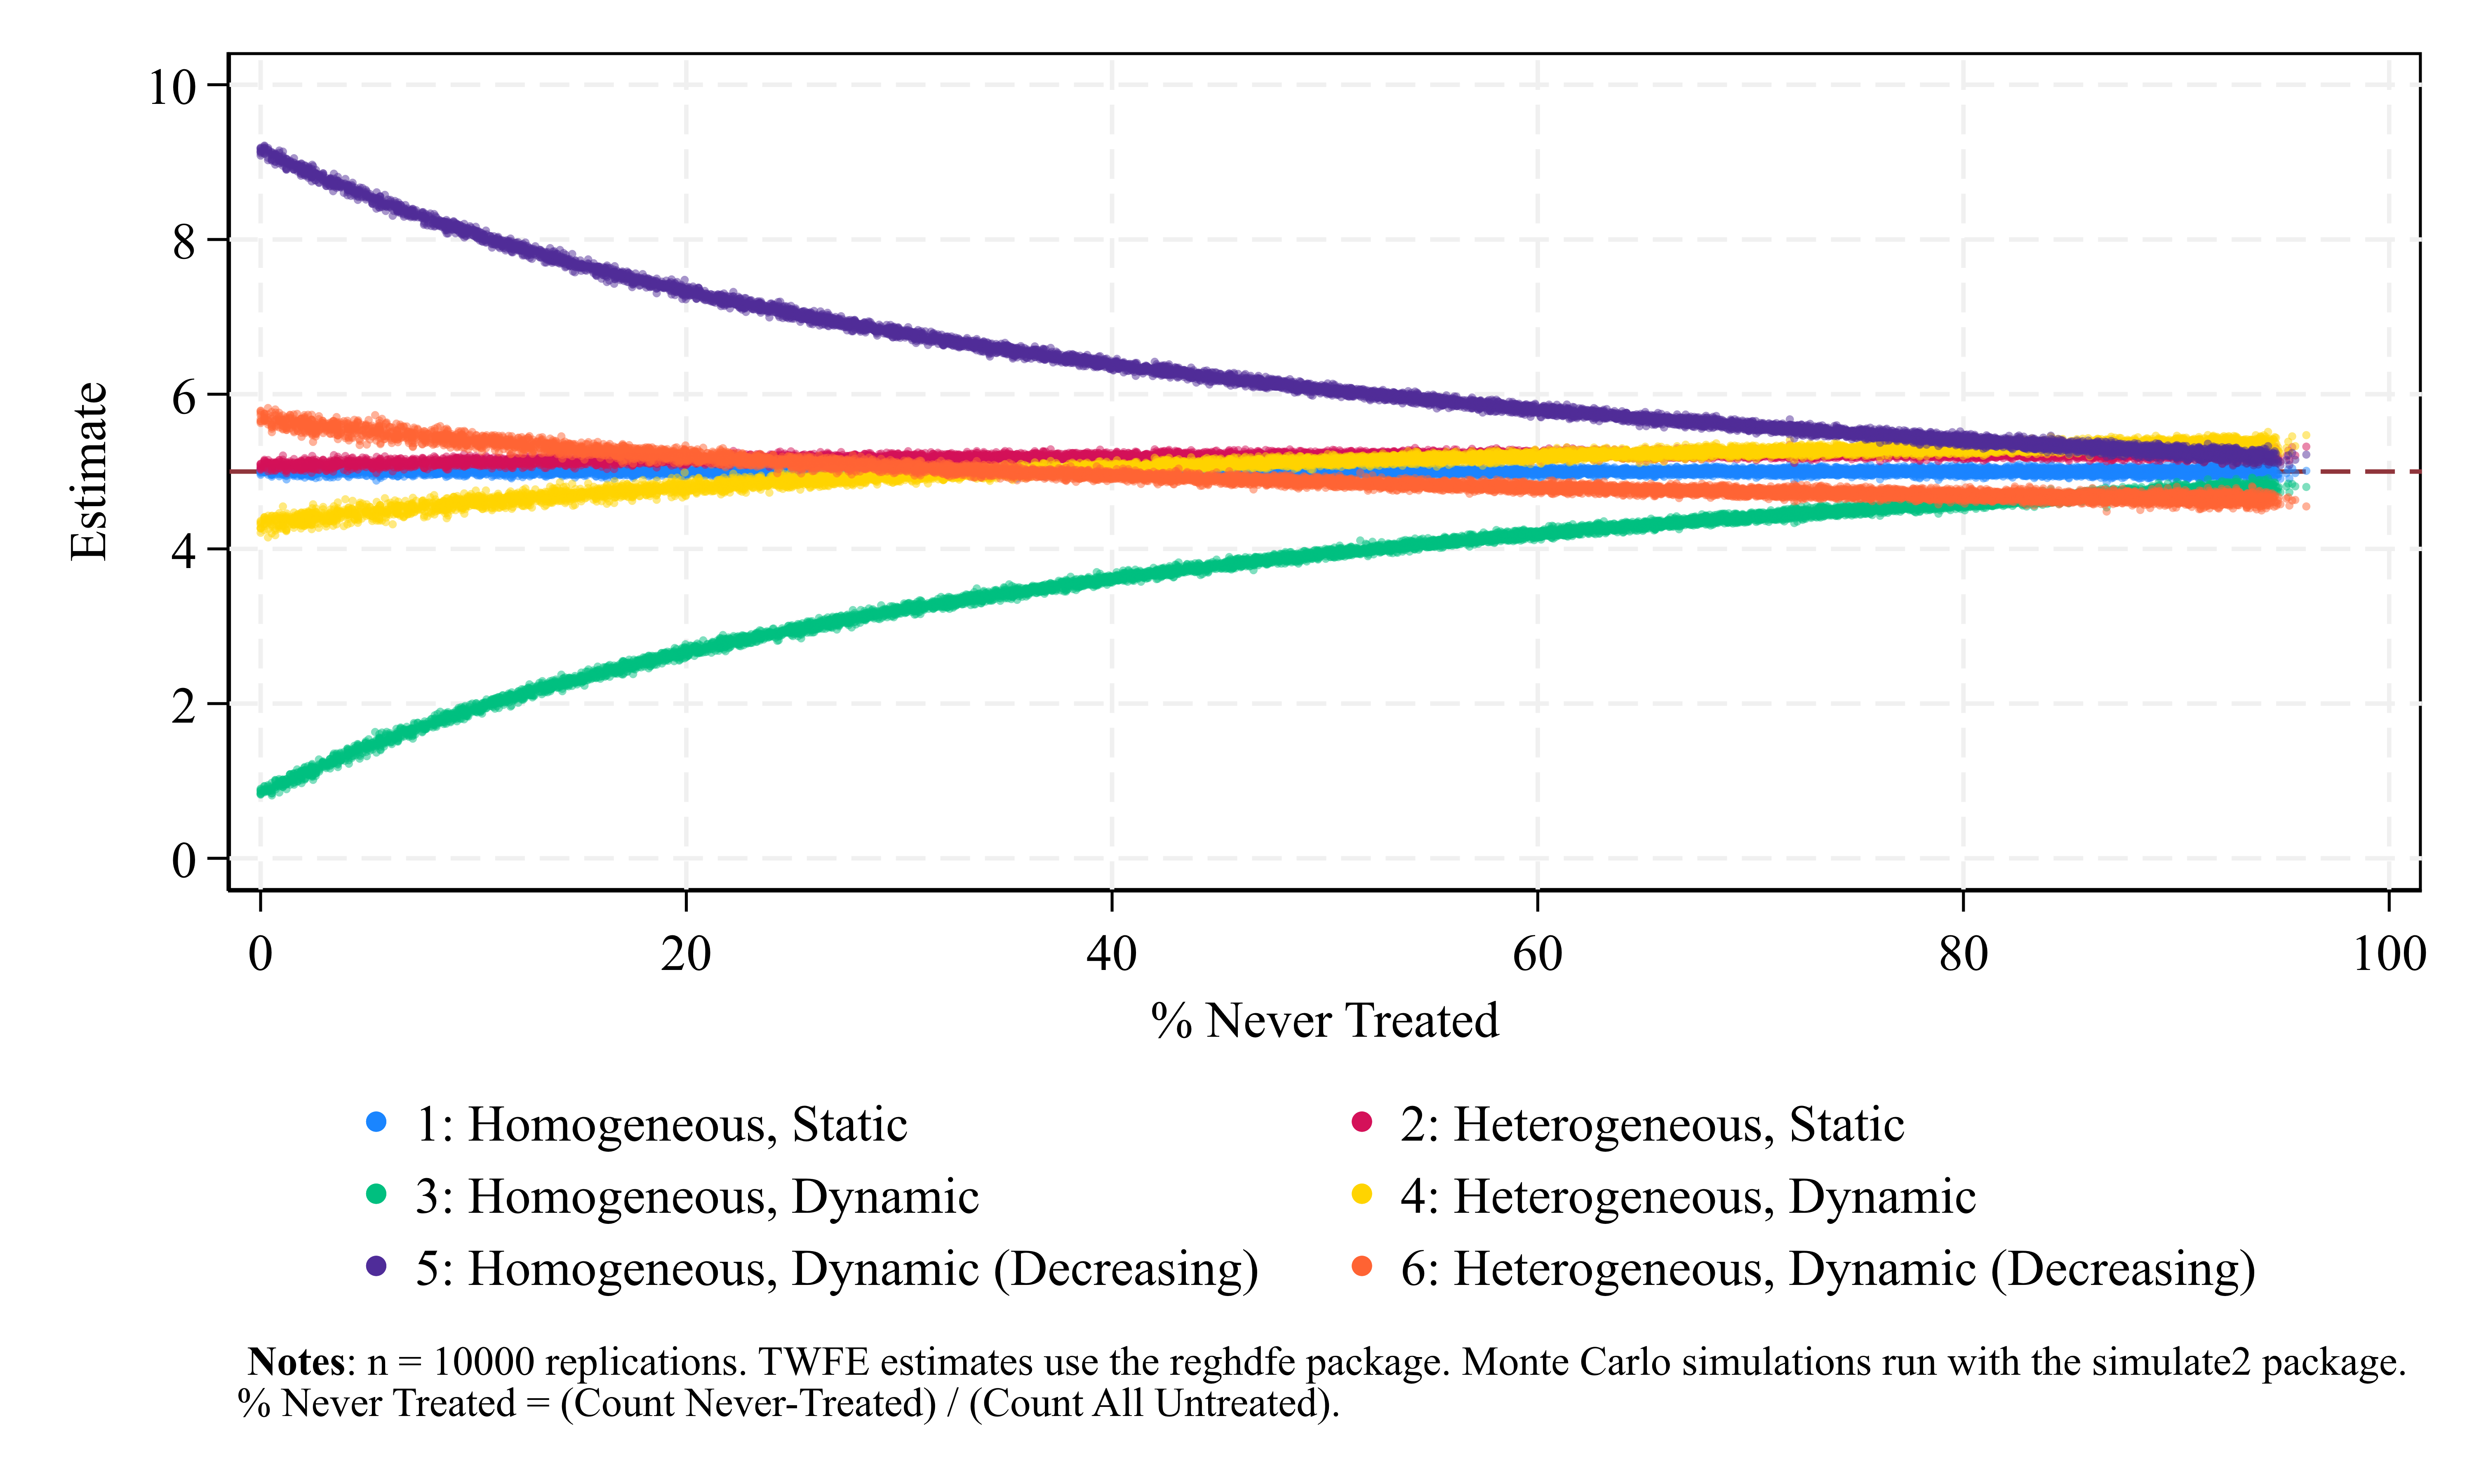
\includegraphics[width=6in]{Figures/TWFE Bias by Percent Never Treated Scatter.png}
    \label{fig:scatter-nevertreat}
\end{figure}

\begin{figure}
    \centering
    \caption{TWFE Bias by Percent Balanced (Scatter Plot)}
    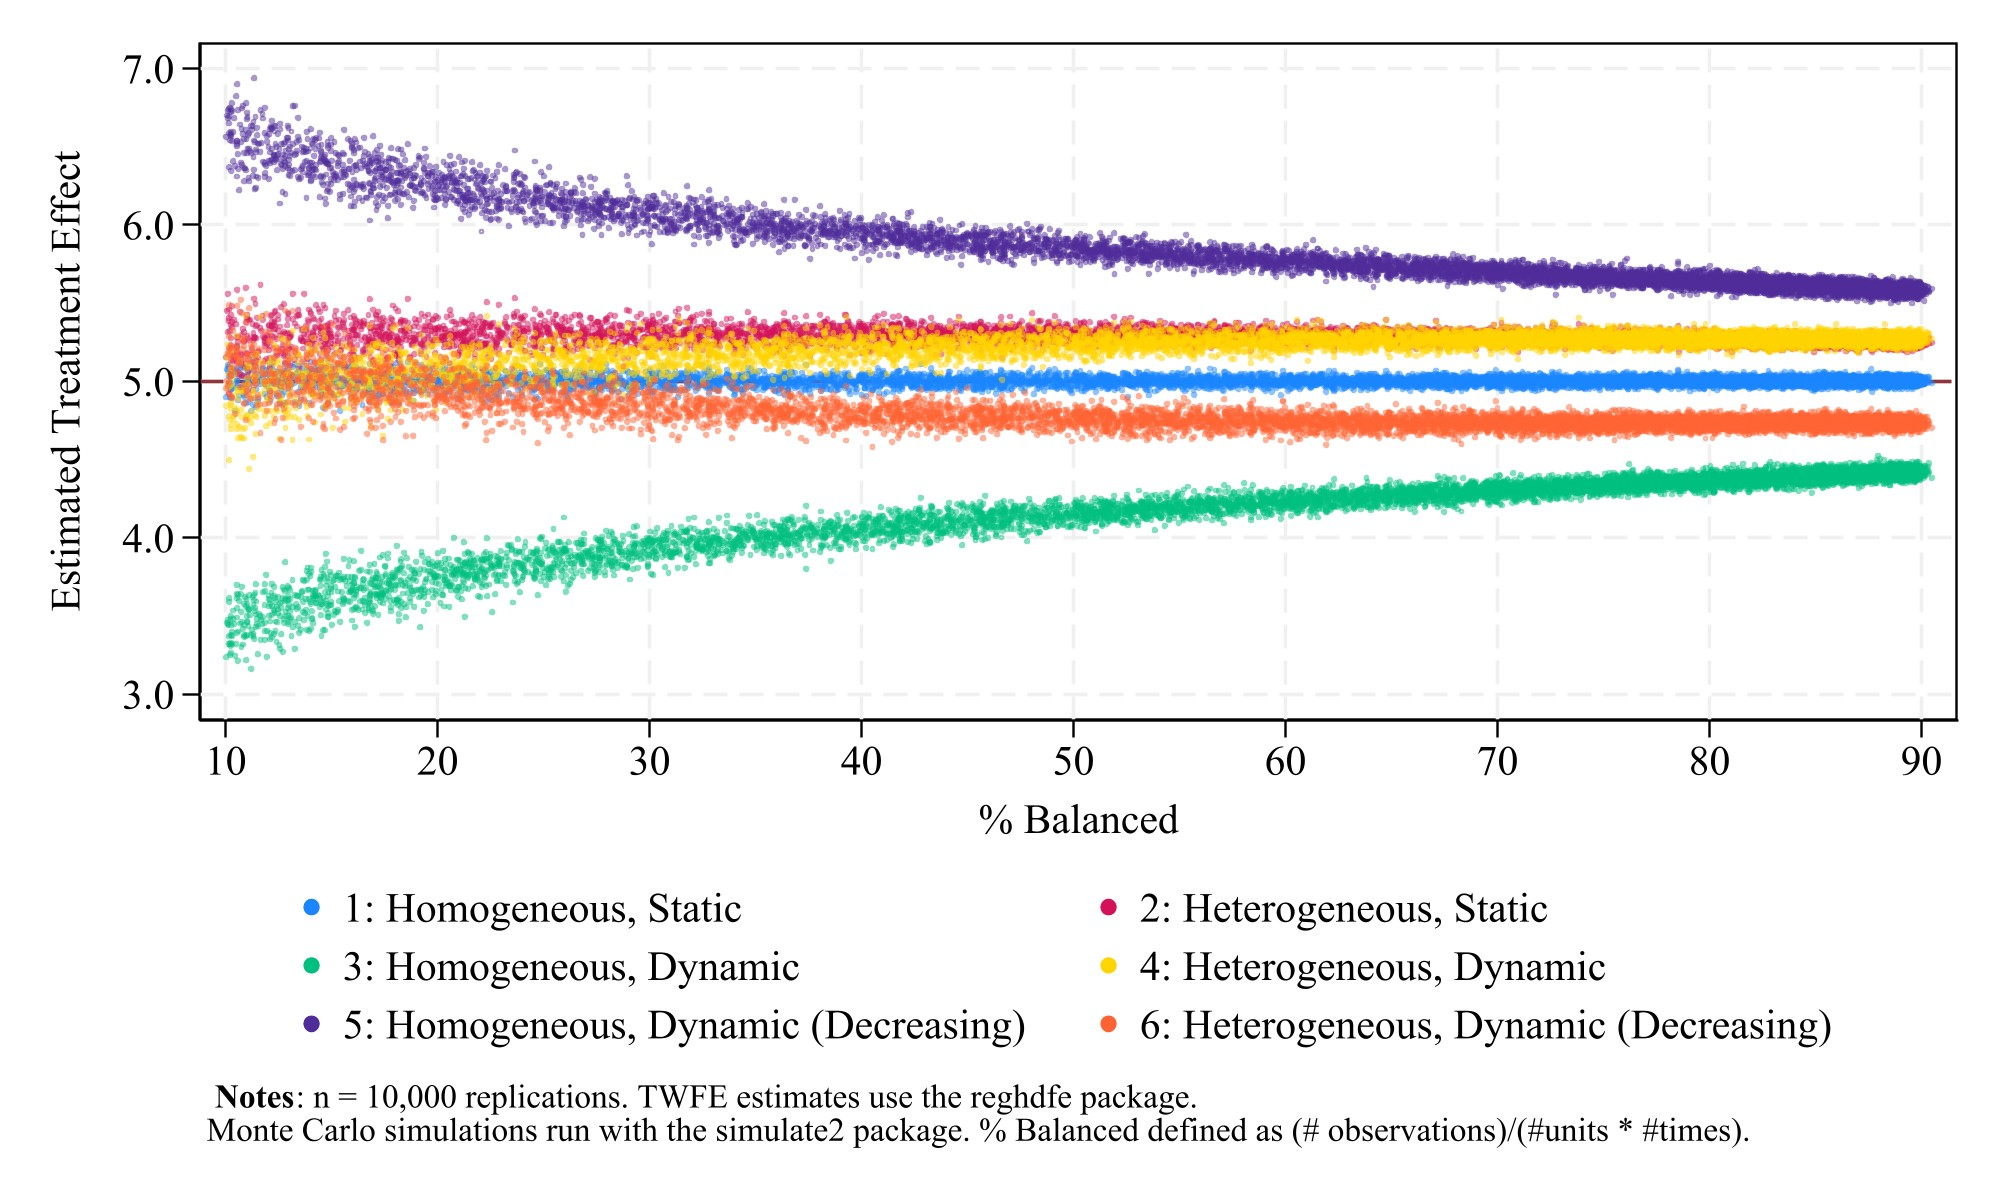
\includegraphics[width=6in]{Figures/TWFE Bias by Percent Balanced Scatter Crop.png}
    \label{fig:scatter-balance}
\end{figure}

\begin{figure}
    \centering
    \caption{Statistical Comparison of DiD Methods with True Average Effect by Percent Balanced (Relative Scale)}
    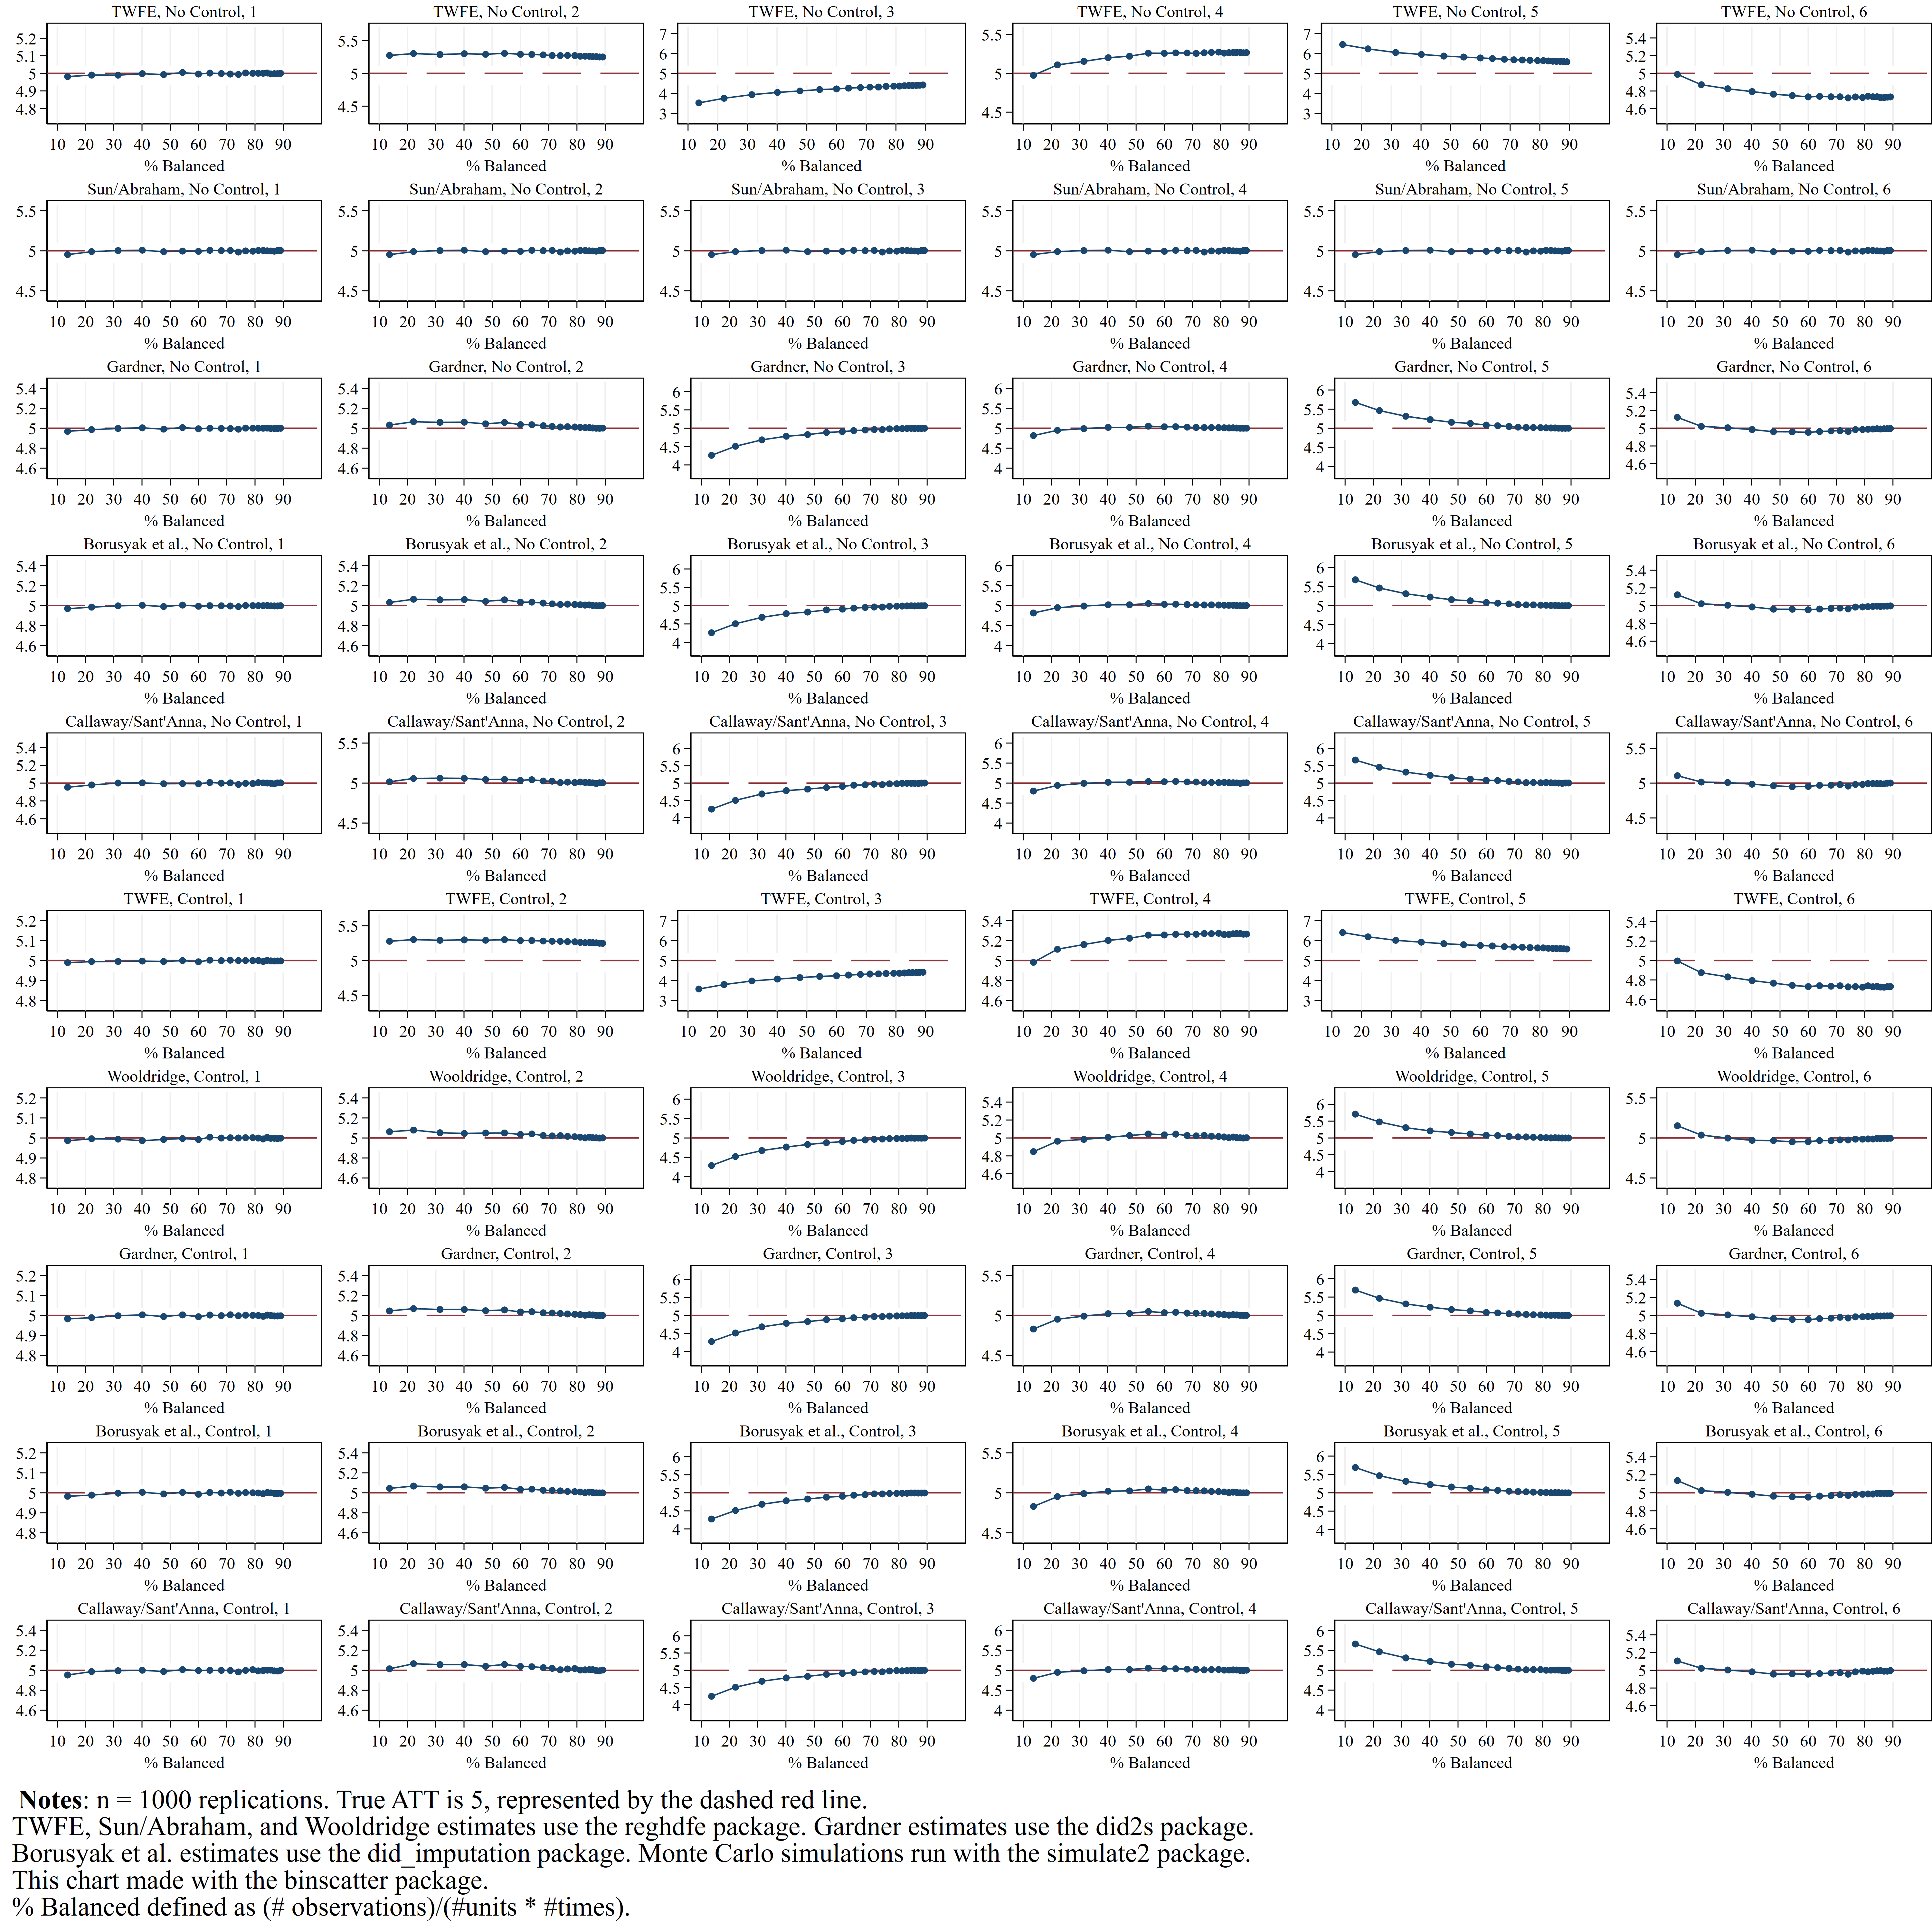
\includegraphics[width=6in]{Figures/Binscatters by Percent Balanced Relative Scale.png}
    \label{fig:bins-relative}
\end{figure}

\begin{figure}
    \centering
    \caption{Statistical Comparison of DiD Methods with True Average Effect by Percent Balanced (Scatter Plot)}
    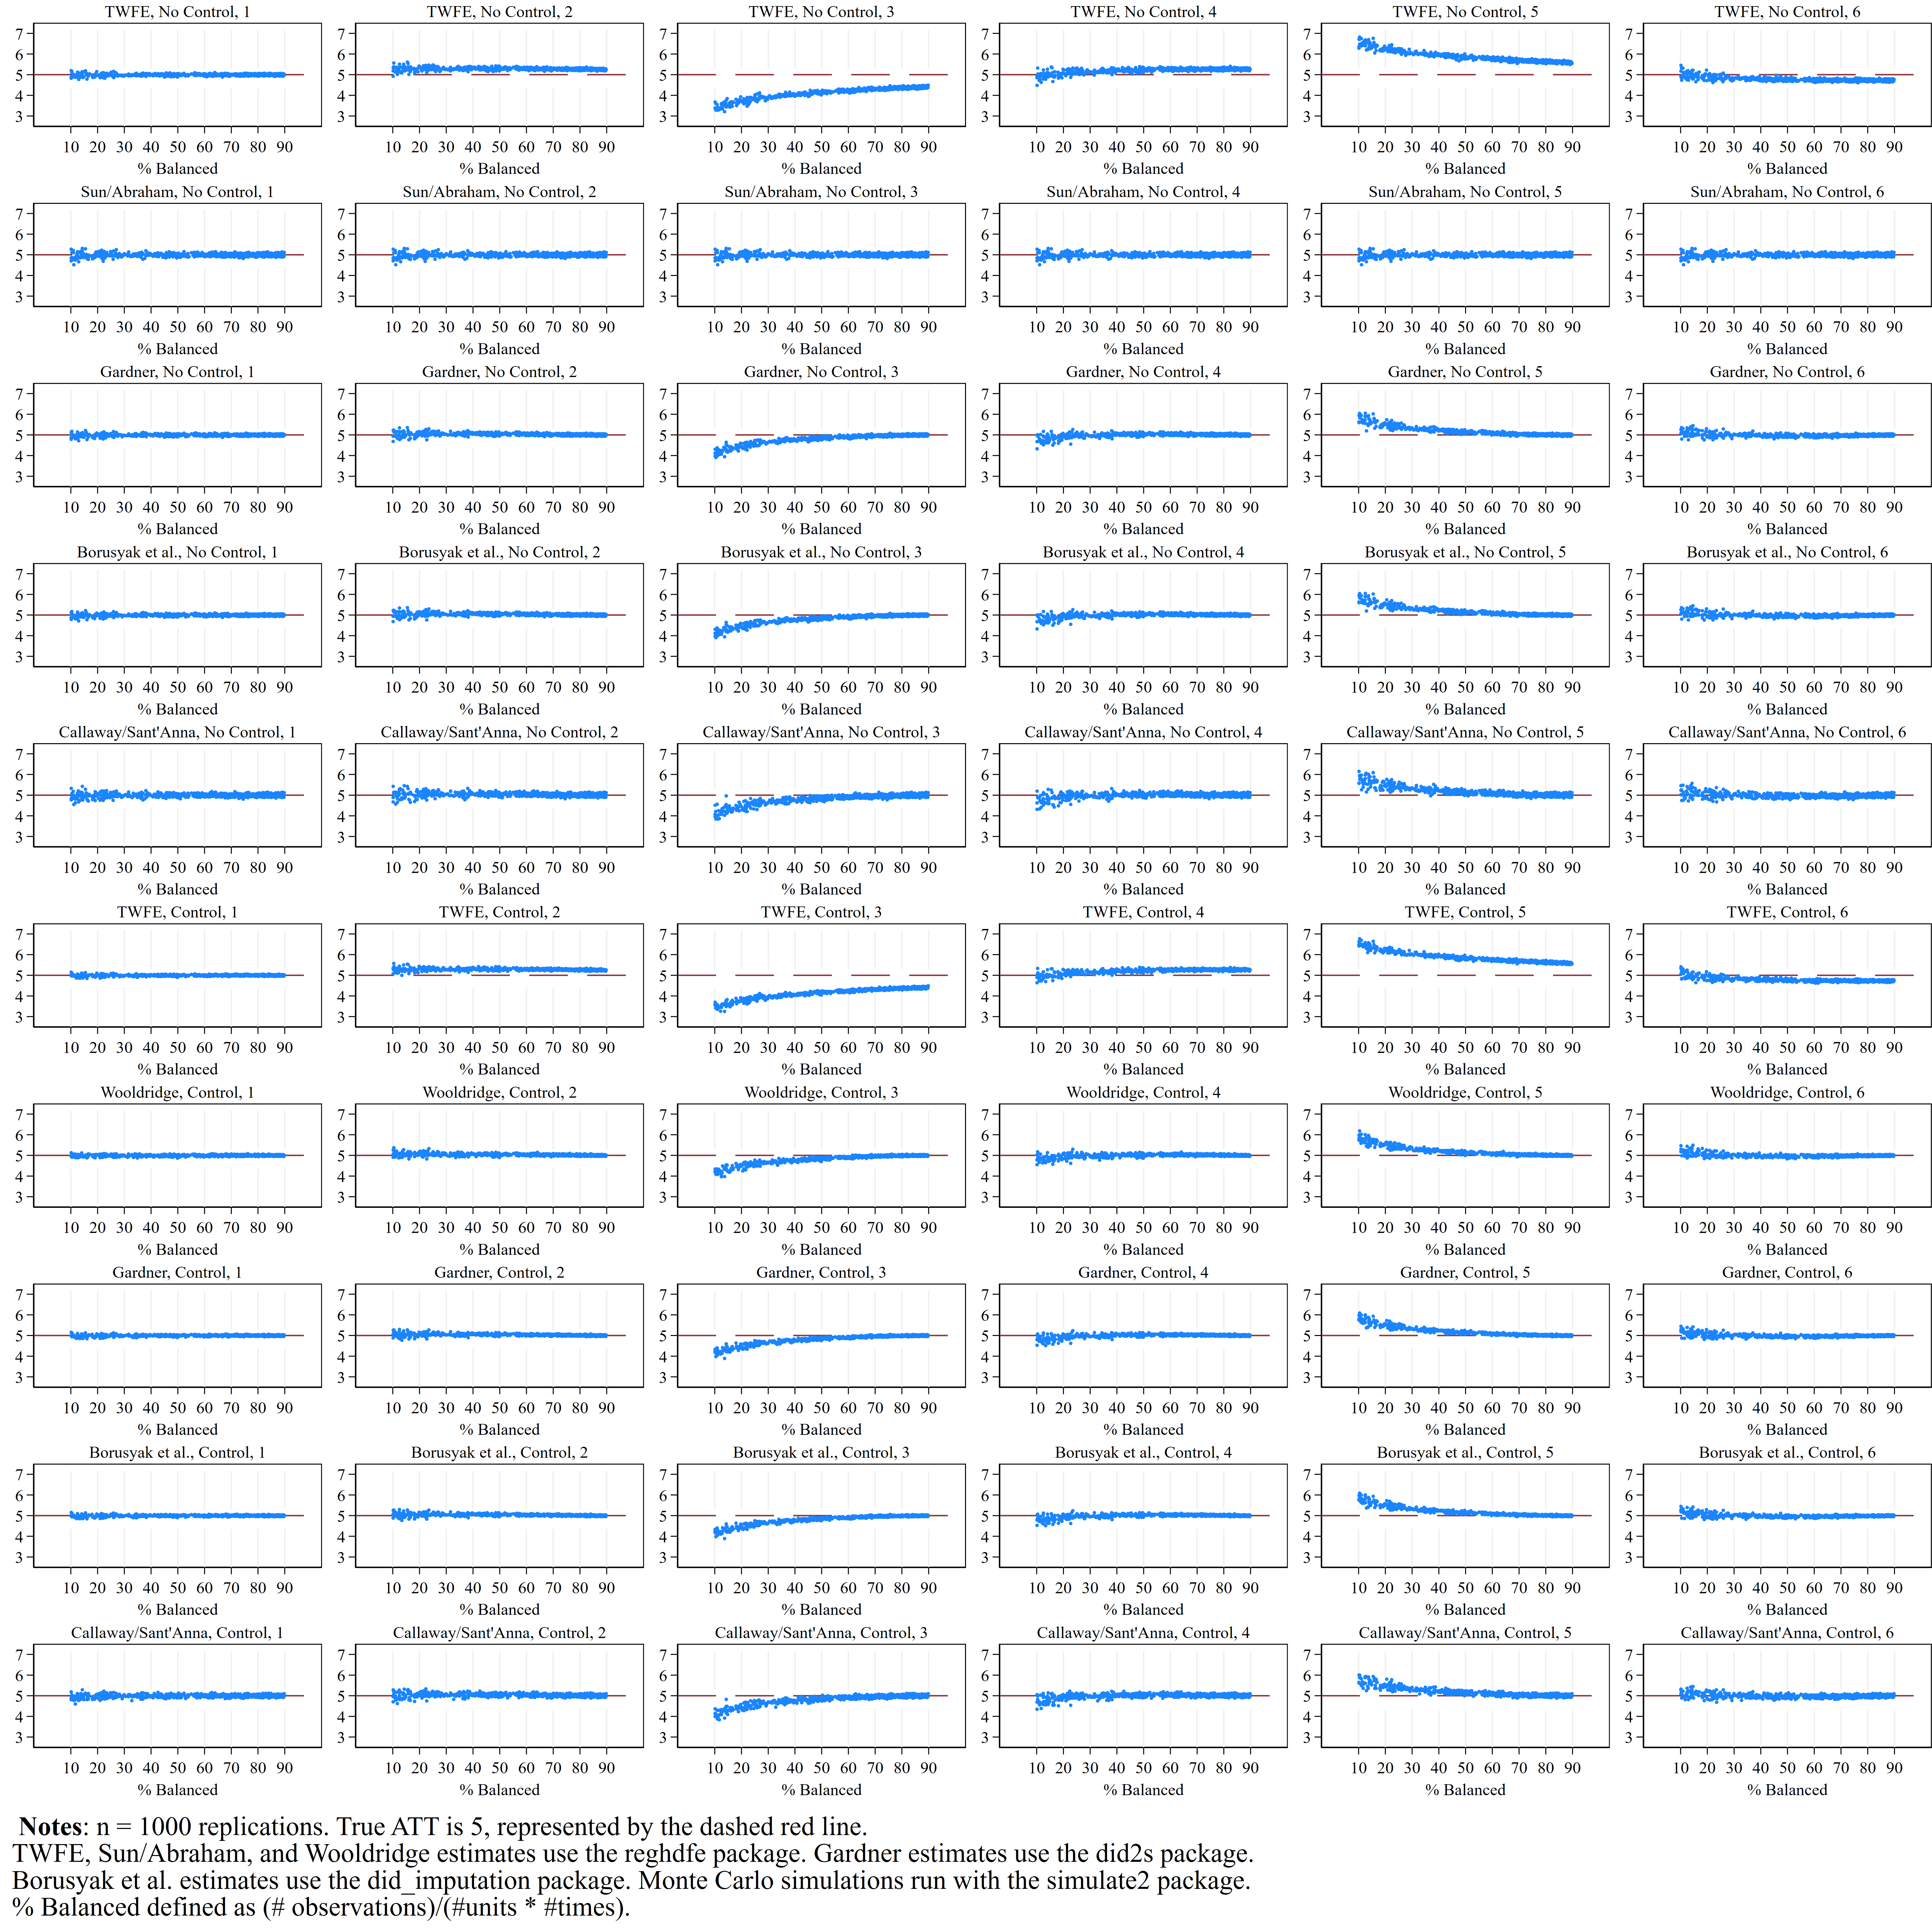
\includegraphics[width=6in]{Figures/Scatters by Percent Balanced Common Scale.png}
    \label{fig:scatters-common}
\end{figure}

\begin{figure}
    \centering
    \caption{Statistical Comparison of DiD Methods with True Average Effect by Percent Balanced (Scatter Plot) (Relative Scale)}
    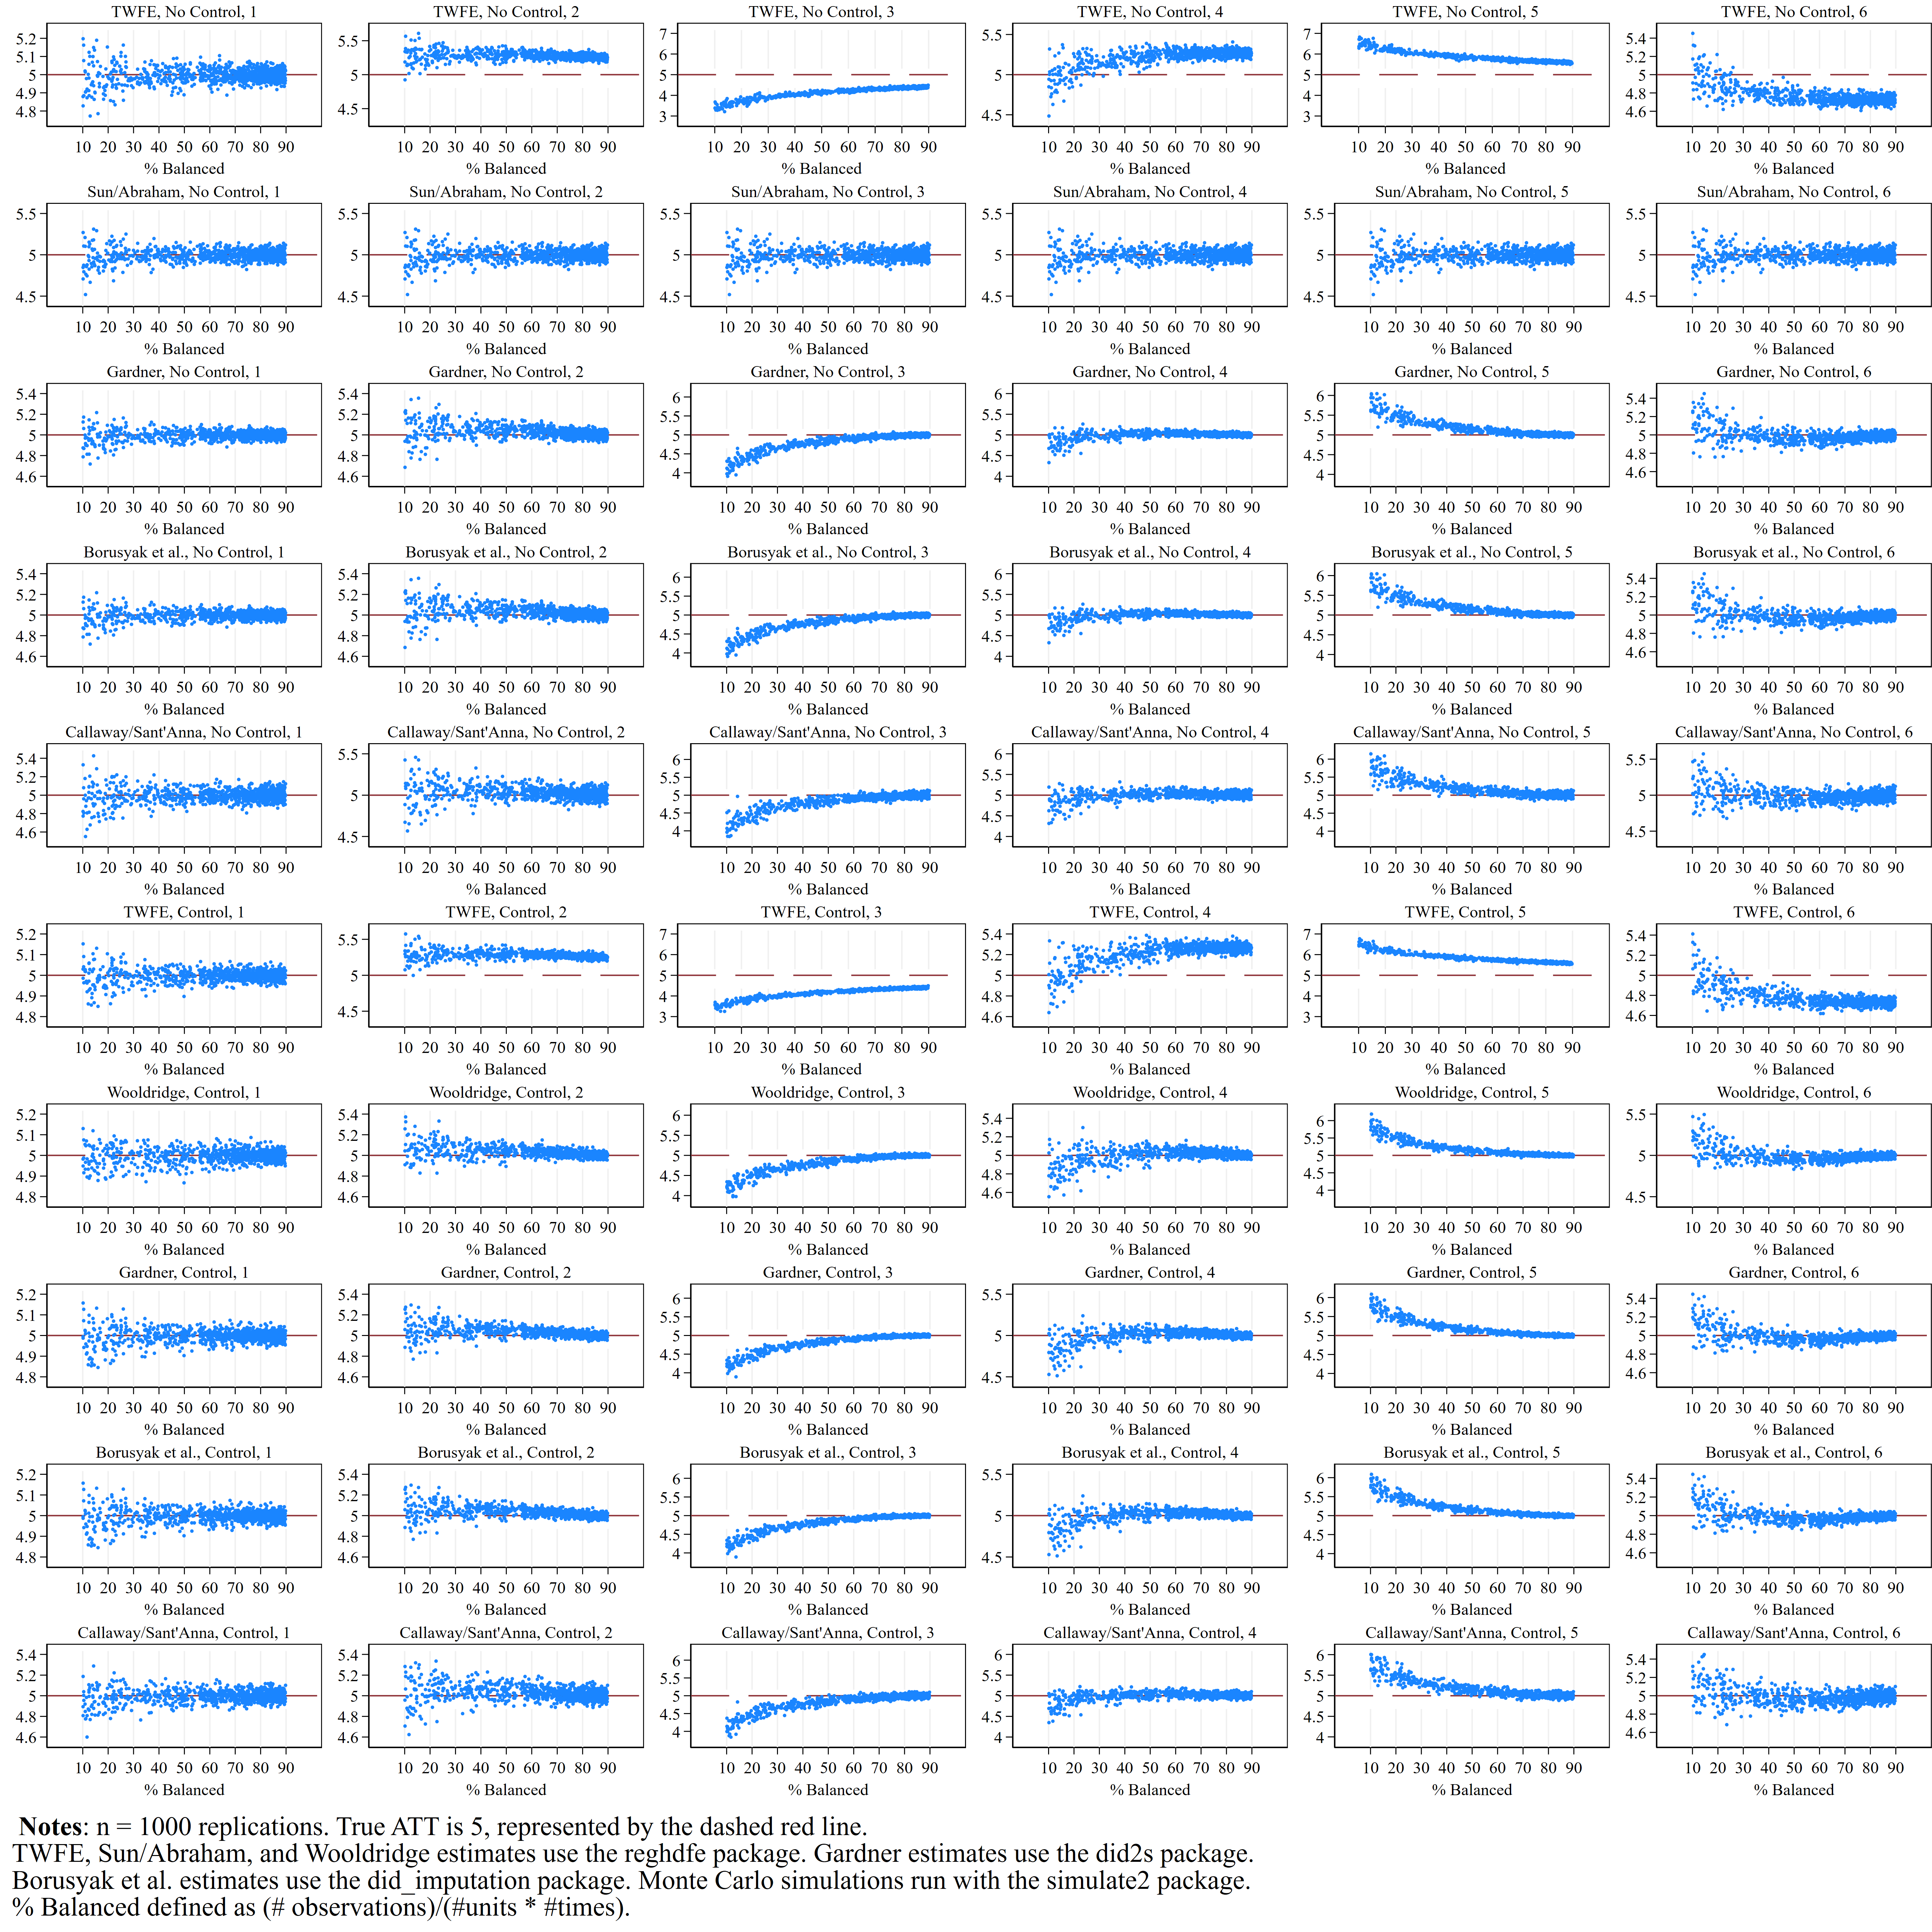
\includegraphics[width=6in]{Figures/Scatters by Percent Balanced Relative Scale.png}
    \label{fig:scatters-relative}
\end{figure}

\begin{figure}
    \centering
    \caption{Average Distribution of Data in Unbalanced Simulations by Treatment Status}
    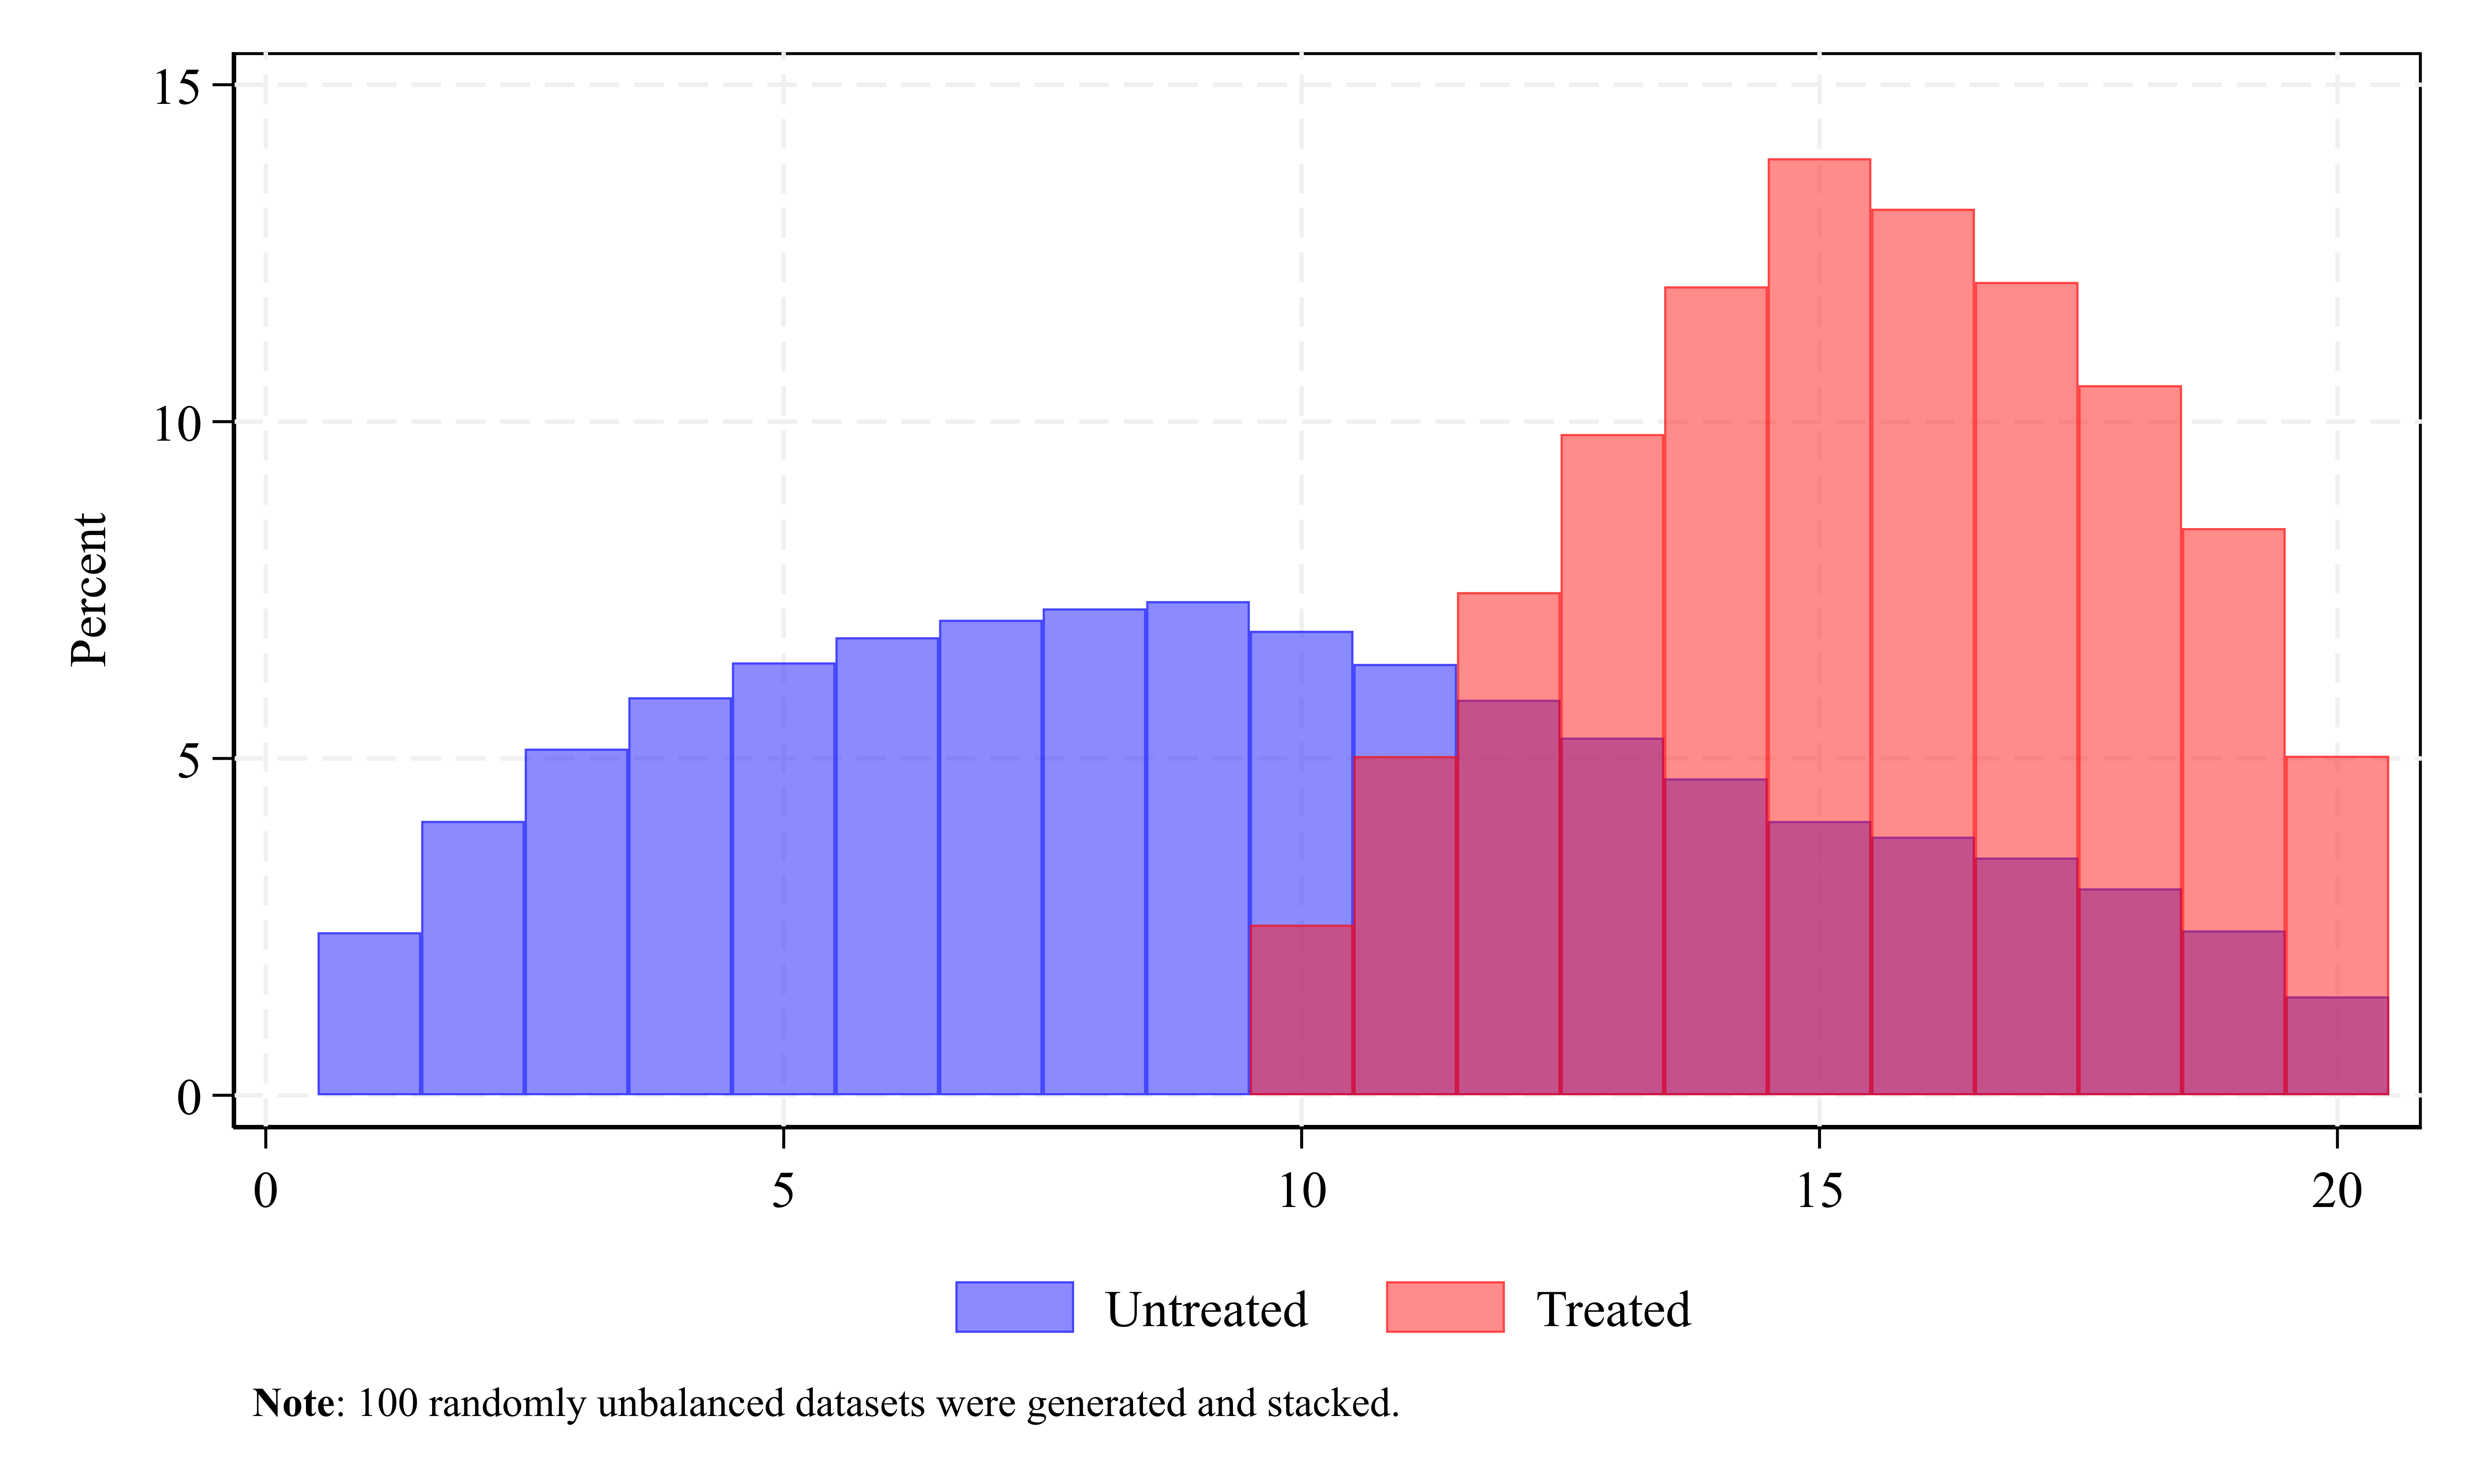
\includegraphics[width=6in]{Figures/Average Distribution of Data in Unbalanced Simulations by Treated.png}
    \label{fig:dist-treat}
\end{figure}

\newgeometry{left=0.5in,bottom=0.5in,right=0.5in,top=0.5in,includefoot}

\begin{landscape}
\begin{table}[htbp]\centering
\def\sym#1{\ifmmode^{#1}\else\(^{#1}\)\fi}
\caption{Regressions of Absolute TWFE Bias}
\scalebox{0.7}{
\begin{tabular}{l*{6}{c}}
\hline\hline
                    &\multicolumn{1}{c}{(1)}&\multicolumn{1}{c}{(2)}&\multicolumn{1}{c}{(3)}&\multicolumn{1}{c}{(4)}&\multicolumn{1}{c}{(5)}&\multicolumn{1}{c}{(6)}\\
                    &\multicolumn{1}{c}{Absolute Bias, Data 1}&\multicolumn{1}{c}{Absolute Bias, Data 2}&\multicolumn{1}{c}{Absolute Bias, Data 3}&\multicolumn{1}{c}{Absolute Bias, Data 4}&\multicolumn{1}{c}{Absolute Bias, Data 5}&\multicolumn{1}{c}{Absolute Bias, Data 6}\\
                    &Coefficient/SE         &Coefficient/SE         &Coefficient/SE         &Coefficient/SE         &Coefficient/SE         &Coefficient/SE         \\
\hline
\% Never-Treated     &      -0.005\sym{***}&      -0.006\sym{***}&      -0.049\sym{***}&      -0.103\sym{***}&      -0.050\sym{***}&      -0.103\sym{***}\\
                    &     (0.000)         &     (0.001)         &     (0.001)         &     (0.001)         &     (0.001)         &     (0.001)         \\
\% Never-Treated Squared&       0.000\sym{***}&       0.000\sym{***}&       0.000\sym{***}&       0.001\sym{***}&       0.000\sym{***}&       0.001\sym{***}\\
                    &     (0.000)         &     (0.000)         &     (0.000)         &     (0.000)         &     (0.000)         &     (0.000)         \\
Count of Units (1000s)&       0.014\sym{*}  &       0.028\sym{***}&       0.260\sym{***}&       0.626\sym{***}&       0.255\sym{***}&       0.617\sym{***}\\
                    &     (0.006)         &     (0.006)         &     (0.008)         &     (0.018)         &     (0.008)         &     (0.018)         \\
First Treatment Time&       0.006\sym{***}&      -0.001         &       0.004\sym{***}&       0.139\sym{***}&       0.003\sym{***}&       0.139\sym{***}\\
                    &     (0.000)         &     (0.000)         &     (0.001)         &     (0.001)         &     (0.001)         &     (0.001)         \\
Longest Treatment Exposure Time&       0.001\sym{**} &       0.037\sym{***}&       0.136\sym{***}&       0.204\sym{***}&       0.136\sym{***}&       0.203\sym{***}\\
                    &     (0.000)         &     (0.001)         &     (0.001)         &     (0.001)         &     (0.001)         &     (0.001)         \\
\% Balanced          &      -0.012\sym{***}&      -0.012\sym{***}&      -0.028\sym{***}&      -0.067\sym{***}&      -0.028\sym{***}&      -0.067\sym{***}\\
                    &     (0.000)         &     (0.000)         &     (0.000)         &     (0.001)         &     (0.000)         &     (0.001)         \\
\% Balanced Squared  &       0.000\sym{***}&       0.000\sym{***}&       0.000\sym{***}&       0.000\sym{***}&       0.000\sym{***}&       0.000\sym{***}\\
                    &     (0.000)         &     (0.000)         &     (0.000)         &     (0.000)         &     (0.000)         &     (0.000)         \\
True Effect Size    &       0.001         &       0.001\sym{*}  &       0.000         &      -0.001         &      -0.000         &      -0.000         \\
                    &     (0.001)         &     (0.001)         &     (0.001)         &     (0.002)         &     (0.001)         &     (0.002)         \\
Individual-Specific Treatment Noise&       0.041\sym{***}&       0.040\sym{***}&       0.027\sym{***}&       0.038\sym{**} &       0.027\sym{***}&       0.028\sym{*}  \\
                    &     (0.004)         &     (0.005)         &     (0.006)         &     (0.013)         &     (0.006)         &     (0.013)         \\
Covariate Treatment Correlation&      -0.000         &       0.147\sym{***}&      -0.534\sym{***}&      -0.299\sym{***}&       0.544\sym{***}&       0.321\sym{***}\\
                    &     (0.007)         &     (0.008)         &     (0.010)         &     (0.021)         &     (0.010)         &     (0.021)         \\
Covariate Size      &       0.000         &       0.000         &       0.000         &       0.003         &       0.001         &       0.003         \\
                    &     (0.001)         &     (0.001)         &     (0.002)         &     (0.003)         &     (0.002)         &     (0.003)         \\
Constant            &       0.504\sym{***}&       0.475\sym{***}&       1.671\sym{***}&       1.271\sym{***}&       1.686\sym{***}&       1.304\sym{***}\\
                    &     (0.016)         &     (0.018)         &     (0.022)         &     (0.048)         &     (0.022)         &     (0.048)         \\
\hline
Row Count           &   49116         &   49116         &   49116         &   49116         &   49116         &   49116         \\
Adjusted R2         &       0.064         &       0.127         &       0.548         &       0.452         &       0.549         &       0.454         \\
F Statistic         &     308.434         &     651.216         &    5412.601         &    3689.500         &    5446.903         &    3719.808         \\
Chi-Squared p-value &       0.000         &       0.000         &       0.000         &       0.000         &       0.000         &       0.000         \\
\hline\hline
\multicolumn{7}{l}{\footnotesize \sym{*} \(p<0.05\), \sym{**} \(p<0.01\), \sym{***} \(p<0.001\)}\\
\end{tabular}
}
\footnotesize  
\vspace{5mm}
    \footnotesize \begin{singlespace*}
        Each observation in this regression is the result of a TWFE model run on data which randomly changes each of the parameters shown here.
    \end{singlespace*}
\end{table}
\end{landscape}

\begin{table}[htbp]\centering
\def\sym#1{\ifmmode^{#1}\else\(^{#1}\)\fi}
\caption{Regressions of Absolute TWFE Bias (Interacted)}
\scalebox{0.5}{
\begin{tabular}{p{4.5in}|*{6}{c}}
\hline\hline
                    &\multicolumn{1}{c}{(1)}&\multicolumn{1}{c}{(2)}&\multicolumn{1}{c}{(3)}&\multicolumn{1}{c}{(4)}&\multicolumn{1}{c}{(5)}&\multicolumn{1}{c}{(6)}\\
                    &\multicolumn{1}{c}{Absolute Bias, Data 1}&\multicolumn{1}{c}{Absolute Bias, Data 2}&\multicolumn{1}{c}{Absolute Bias, Data 3}&\multicolumn{1}{c}{Absolute Bias, Data 4}&\multicolumn{1}{c}{Absolute Bias, Data 5}&\multicolumn{1}{c}{Absolute Bias, Data 6}\\
                    &Coefficient/SE         &Coefficient/SE         &Coefficient/SE         &Coefficient/SE         &Coefficient/SE         &Coefficient/SE         \\
\hline
\% Never-Treated     &      -0.010\sym{***}&      -0.010\sym{***}&      -0.018\sym{***}&       0.038\sym{***}&      -0.019\sym{***}&       0.042\sym{***}\\
                    &     (0.002)         &     (0.002)         &     (0.002)         &     (0.004)         &     (0.002)         &     (0.004)         \\
\% Never-Treated Squared&       0.000\sym{***}&       0.000\sym{***}&       0.000\sym{***}&      -0.000         &       0.000\sym{***}&      -0.000\sym{*}  \\
                    &     (0.000)         &     (0.000)         &     (0.000)         &     (0.000)         &     (0.000)         &     (0.000)         \\
Count of Units (1000s)&       0.006         &       0.007         &       0.204\sym{***}&       0.361\sym{***}&       0.190\sym{***}&       0.388\sym{***}\\
                    &     (0.018)         &     (0.019)         &     (0.021)         &     (0.045)         &     (0.021)         &     (0.045)         \\
First Treatment Time&       0.003\sym{**} &      -0.001         &      -0.020\sym{***}&       0.275\sym{***}&      -0.021\sym{***}&       0.275\sym{***}\\
                    &     (0.001)         &     (0.001)         &     (0.001)         &     (0.003)         &     (0.001)         &     (0.003)         \\
Longest Treatment Exposure Time&      -0.001         &       0.028\sym{***}&       0.282\sym{***}&       0.447\sym{***}&       0.282\sym{***}&       0.448\sym{***}\\
                    &     (0.001)         &     (0.002)         &     (0.002)         &     (0.004)         &     (0.002)         &     (0.004)         \\
\% Balanced          &      -0.010\sym{***}&      -0.009\sym{***}&      -0.020\sym{***}&      -0.071\sym{***}&      -0.020\sym{***}&      -0.071\sym{***}\\
                    &     (0.001)         &     (0.001)         &     (0.001)         &     (0.002)         &     (0.001)         &     (0.002)         \\
\% Balanced Squared  &       0.000\sym{***}&       0.000\sym{***}&       0.000\sym{***}&       0.000\sym{***}&       0.000\sym{***}&       0.000\sym{***}\\
                    &     (0.000)         &     (0.000)         &     (0.000)         &     (0.000)         &     (0.000)         &     (0.000)         \\
True Effect Size    &       0.001         &       0.002         &      -0.001         &      -0.008         &      -0.001         &      -0.008         \\
                    &     (0.002)         &     (0.002)         &     (0.002)         &     (0.005)         &     (0.002)         &     (0.005)         \\
Individual-Specific Treatment Noise&       0.065\sym{***}&       0.063\sym{***}&       0.041\sym{**} &       0.114\sym{***}&       0.042\sym{**} &       0.090\sym{**} \\
                    &     (0.013)         &     (0.014)         &     (0.015)         &     (0.033)         &     (0.015)         &     (0.033)         \\
True Effect Size $\times$ Individual-Specific Treatment Noise&       0.003         &       0.003         &       0.001         &       0.004         &       0.002         &       0.004         \\
                    &     (0.002)         &     (0.002)         &     (0.002)         &     (0.004)         &     (0.002)         &     (0.004)         \\
Covariate Treatment Correlation&       0.056\sym{**} &       0.119\sym{***}&      -0.794\sym{***}&      -0.537\sym{***}&       0.797\sym{***}&       0.456\sym{***}\\
                    &     (0.021)         &     (0.023)         &     (0.025)         &     (0.054)         &     (0.025)         &     (0.054)         \\
Covariate Size      &       0.001         &       0.003         &       0.006         &      -0.024\sym{**} &       0.003         &      -0.017\sym{*}  \\
                    &     (0.003)         &     (0.004)         &     (0.004)         &     (0.008)         &     (0.004)         &     (0.008)         \\
Covariate Treatment Correlation $\times$ Covariate Size&      -0.002         &       0.001         &       0.010         &      -0.001         &       0.010         &       0.002         \\
                    &     (0.007)         &     (0.007)         &     (0.008)         &     (0.017)         &     (0.008)         &     (0.017)         \\
\% Never-Treated $\times$ Count of Units (1000s)&      -0.000         &      -0.000         &       0.003\sym{***}&       0.015\sym{***}&       0.003\sym{***}&       0.013\sym{***}\\
                    &     (0.001)         &     (0.001)         &     (0.001)         &     (0.002)         &     (0.001)         &     (0.002)         \\
\% Never-Treated $\times$ First Treatment Time&       0.000         &      -0.000         &       0.001\sym{***}&      -0.004\sym{***}&       0.001\sym{***}&      -0.004\sym{***}\\
                    &     (0.000)         &     (0.000)         &     (0.000)         &     (0.000)         &     (0.000)         &     (0.000)         \\
\% Never-Treated $\times$ Longest Treatment Exposure Time&       0.000         &       0.000\sym{***}&      -0.004\sym{***}&      -0.008\sym{***}&      -0.005\sym{***}&      -0.008\sym{***}\\
                    &     (0.000)         &     (0.000)         &     (0.000)         &     (0.000)         &     (0.000)         &     (0.000)         \\
\% Never-Treated $\times$ \% Balanced&       0.000\sym{***}&       0.000\sym{**} &      -0.000\sym{*}  &      -0.000         &      -0.000\sym{*}  &      -0.000         \\
                    &     (0.000)         &     (0.000)         &     (0.000)         &     (0.000)         &     (0.000)         &     (0.000)         \\
\% Never-Treated $\times$ \% Balanced Squared&      -0.000\sym{***}&      -0.000\sym{**} &       0.000         &      -0.000\sym{***}&      -0.000         &      -0.000\sym{***}\\
                    &     (0.000)         &     (0.000)         &     (0.000)         &     (0.000)         &     (0.000)         &     (0.000)         \\
\% Never-Treated $\times$ True Effect Size&      -0.000         &      -0.000         &      -0.000         &       0.000         &      -0.000         &       0.000         \\
                    &     (0.000)         &     (0.000)         &     (0.000)         &     (0.000)         &     (0.000)         &     (0.000)         \\
\% Never-Treated $\times$ Individual-Specific Treatment Noise&      -0.003\sym{***}&      -0.003\sym{***}&      -0.002\sym{***}&      -0.006\sym{***}&      -0.003\sym{***}&      -0.005\sym{***}\\
                    &     (0.001)         &     (0.001)         &     (0.001)         &     (0.002)         &     (0.001)         &     (0.002)         \\
\% Never-Treated $\times$ True Effect Size $\times$ Individual-Specific Treatment Noise&      -0.000         &      -0.000         &      -0.000         &      -0.000         &      -0.000         &      -0.000         \\
                    &     (0.000)         &     (0.000)         &     (0.000)         &     (0.000)         &     (0.000)         &     (0.000)         \\
\% Never-Treated $\times$ Covariate Treatment Correlation&      -0.003\sym{**} &       0.001         &       0.004\sym{***}&       0.003         &      -0.006\sym{***}&      -0.001         \\
                    &     (0.001)         &     (0.001)         &     (0.001)         &     (0.002)         &     (0.001)         &     (0.002)         \\
\% Never-Treated $\times$ Covariate Size&      -0.000         &      -0.000         &      -0.000         &       0.001\sym{**} &      -0.000         &       0.001\sym{*}  \\
                    &     (0.000)         &     (0.000)         &     (0.000)         &     (0.000)         &     (0.000)         &     (0.000)         \\
\% Never-Treated $\times$ Covariate Treatment Correlation $\times$ Covariate Size&       0.000         &       0.001         &      -0.000         &      -0.000         &       0.000         &      -0.000         \\
                    &     (0.000)         &     (0.000)         &     (0.000)         &     (0.001)         &     (0.000)         &     (0.001)         \\
\% Never-Treated Squared $\times$ Count of Units (1000s)&       0.000         &       0.000         &      -0.000\sym{***}&      -0.000\sym{***}&      -0.000\sym{**} &      -0.000\sym{***}\\
                    &     (0.000)         &     (0.000)         &     (0.000)         &     (0.000)         &     (0.000)         &     (0.000)         \\
\% Never-Treated Squared $\times$ First Treatment Time&       0.000         &       0.000         &      -0.000\sym{***}&       0.000\sym{***}&      -0.000\sym{***}&       0.000\sym{***}\\
                    &     (0.000)         &     (0.000)         &     (0.000)         &     (0.000)         &     (0.000)         &     (0.000)         \\
\% Never-Treated Squared $\times$ Longest Treatment Exposure Time&      -0.000         &      -0.000\sym{*}  &       0.000\sym{***}&       0.000\sym{***}&       0.000\sym{***}&       0.000\sym{***}\\
                    &     (0.000)         &     (0.000)         &     (0.000)         &     (0.000)         &     (0.000)         &     (0.000)         \\
\% Never-Treated Squared $\times$ \% Balanced&      -0.000\sym{***}&      -0.000\sym{***}&      -0.000         &       0.000\sym{*}  &      -0.000         &       0.000\sym{*}  \\
                    &     (0.000)         &     (0.000)         &     (0.000)         &     (0.000)         &     (0.000)         &     (0.000)         \\
\% Never-Treated Squared $\times$ \% Balanced Squared&       0.000\sym{***}&       0.000\sym{***}&       0.000\sym{*}  &       0.000\sym{**} &       0.000\sym{**} &       0.000\sym{*}  \\
                    &     (0.000)         &     (0.000)         &     (0.000)         &     (0.000)         &     (0.000)         &     (0.000)         \\
\% Never-Treated Squared $\times$ True Effect Size&       0.000         &       0.000         &       0.000         &      -0.000         &       0.000         &      -0.000         \\
                    &     (0.000)         &     (0.000)         &     (0.000)         &     (0.000)         &     (0.000)         &     (0.000)         \\
\% Never-Treated Squared $\times$ Individual-Specific Treatment Noise&       0.000\sym{***}&       0.000\sym{***}&       0.000\sym{***}&       0.000\sym{***}&       0.000\sym{***}&       0.000\sym{***}\\
                    &     (0.000)         &     (0.000)         &     (0.000)         &     (0.000)         &     (0.000)         &     (0.000)         \\
\% Never-Treated Squared $\times$ True Effect Size $\times$ Individual-Specific Treatment Noise&       0.000         &       0.000         &      -0.000         &       0.000         &      -0.000         &       0.000         \\
                    &     (0.000)         &     (0.000)         &     (0.000)         &     (0.000)         &     (0.000)         &     (0.000)         \\
\% Never-Treated Squared $\times$ Covariate Treatment Correlation&       0.000\sym{*}  &      -0.000         &       0.000         &       0.000         &       0.000         &      -0.000         \\
                    &     (0.000)         &     (0.000)         &     (0.000)         &     (0.000)         &     (0.000)         &     (0.000)         \\
\% Never-Treated Squared $\times$ Covariate Size&       0.000         &       0.000         &       0.000         &      -0.000\sym{**} &       0.000         &      -0.000         \\
                    &     (0.000)         &     (0.000)         &     (0.000)         &     (0.000)         &     (0.000)         &     (0.000)         \\
\% Never-Treated Squared $\times$ Covariate Treatment Correlation $\times$ Covariate Size&      -0.000         &      -0.000         &      -0.000         &       0.000         &      -0.000         &       0.000         \\
                    &     (0.000)         &     (0.000)         &     (0.000)         &     (0.000)         &     (0.000)         &     (0.000)         \\
Constant            &       0.529\sym{***}&       0.510\sym{***}&       0.515\sym{***}&      -3.345\sym{***}&       0.556\sym{***}&      -3.377\sym{***}\\
                    &     (0.037)         &     (0.041)         &     (0.044)         &     (0.096)         &     (0.044)         &     (0.096)         \\
\hline
Row Count           &   49116         &   49116         &   49116         &   49116         &   49116         &   49116         \\
Adjusted R2         &       0.076         &       0.137         &       0.681         &       0.602         &       0.685         &       0.605         \\
F Statistic         &     117.023         &     223.488         &    3001.133         &    2125.695         &    3058.231         &    2147.166         \\
Chi-Squared p-value &       0.000         &       0.000         &       0.000         &       0.000         &       0.000         &       0.000         \\
\hline\hline
\multicolumn{7}{l}{\footnotesize \sym{*} \(p<0.05\), \sym{**} \(p<0.01\), \sym{***} \(p<0.001\)}\\
\end{tabular}
}
\footnotesize  
\vspace{5mm}
    \footnotesize \begin{singlespace*}
        Each observation in this regression is the result of a TWFE model run on data which randomly changes each of the parameters shown here.
    \end{singlespace*}
\end{table}

\end{document}